% Options for packages loaded elsewhere
\PassOptionsToPackage{unicode}{hyperref}
\PassOptionsToPackage{hyphens}{url}
%
\documentclass[
  man, donotrepeattitle,floatsintext]{apa7}
\usepackage{amsmath,amssymb}
\usepackage{iftex}
\ifPDFTeX
  \usepackage[T1]{fontenc}
  \usepackage[utf8]{inputenc}
  \usepackage{textcomp} % provide euro and other symbols
\else % if luatex or xetex
  \usepackage{unicode-math} % this also loads fontspec
  \defaultfontfeatures{Scale=MatchLowercase}
  \defaultfontfeatures[\rmfamily]{Ligatures=TeX,Scale=1}
\fi
\usepackage{lmodern}
\ifPDFTeX\else
  % xetex/luatex font selection
\fi
% Use upquote if available, for straight quotes in verbatim environments
\IfFileExists{upquote.sty}{\usepackage{upquote}}{}
\IfFileExists{microtype.sty}{% use microtype if available
  \usepackage[]{microtype}
  \UseMicrotypeSet[protrusion]{basicmath} % disable protrusion for tt fonts
}{}
\makeatletter
\@ifundefined{KOMAClassName}{% if non-KOMA class
  \IfFileExists{parskip.sty}{%
    \usepackage{parskip}
  }{% else
    \setlength{\parindent}{0pt}
    \setlength{\parskip}{6pt plus 2pt minus 1pt}}
}{% if KOMA class
  \KOMAoptions{parskip=half}}
\makeatother
\usepackage{xcolor}
\usepackage{graphicx}
\makeatletter
\def\maxwidth{\ifdim\Gin@nat@width>\linewidth\linewidth\else\Gin@nat@width\fi}
\def\maxheight{\ifdim\Gin@nat@height>\textheight\textheight\else\Gin@nat@height\fi}
\makeatother
% Scale images if necessary, so that they will not overflow the page
% margins by default, and it is still possible to overwrite the defaults
% using explicit options in \includegraphics[width, height, ...]{}
\setkeys{Gin}{width=\maxwidth,height=\maxheight,keepaspectratio}
% Set default figure placement to htbp
\makeatletter
\def\fps@figure{htbp}
\makeatother
\setlength{\emergencystretch}{3em} % prevent overfull lines
\providecommand{\tightlist}{%
  \setlength{\itemsep}{0pt}\setlength{\parskip}{0pt}}
\setcounter{secnumdepth}{5}
% Make \paragraph and \subparagraph free-standing
\makeatletter
\ifx\paragraph\undefined\else
  \let\oldparagraph\paragraph
  \renewcommand{\paragraph}{
    \@ifstar
      \xxxParagraphStar
      \xxxParagraphNoStar
  }
  \newcommand{\xxxParagraphStar}[1]{\oldparagraph*{#1}\mbox{}}
  \newcommand{\xxxParagraphNoStar}[1]{\oldparagraph{#1}\mbox{}}
\fi
\ifx\subparagraph\undefined\else
  \let\oldsubparagraph\subparagraph
  \renewcommand{\subparagraph}{
    \@ifstar
      \xxxSubParagraphStar
      \xxxSubParagraphNoStar
  }
  \newcommand{\xxxSubParagraphStar}[1]{\oldsubparagraph*{#1}\mbox{}}
  \newcommand{\xxxSubParagraphNoStar}[1]{\oldsubparagraph{#1}\mbox{}}
\fi
\makeatother
% definitions for citeproc citations
\NewDocumentCommand\citeproctext{}{}
\NewDocumentCommand\citeproc{mm}{%
  \begingroup\def\citeproctext{#2}\cite{#1}\endgroup}
\makeatletter
 % allow citations to break across lines
 \let\@cite@ofmt\@firstofone
 % avoid brackets around text for \cite:
 \def\@biblabel#1{}
 \def\@cite#1#2{{#1\if@tempswa , #2\fi}}
\makeatother
\newlength{\cslhangindent}
\setlength{\cslhangindent}{1.5em}
\newlength{\csllabelwidth}
\setlength{\csllabelwidth}{3em}
\newenvironment{CSLReferences}[2] % #1 hanging-indent, #2 entry-spacing
 {\begin{list}{}{%
  \setlength{\itemindent}{0pt}
  \setlength{\leftmargin}{0pt}
  \setlength{\parsep}{0pt}
  % turn on hanging indent if param 1 is 1
  \ifodd #1
   \setlength{\leftmargin}{\cslhangindent}
   \setlength{\itemindent}{-1\cslhangindent}
  \fi
  % set entry spacing
  \setlength{\itemsep}{#2\baselineskip}}}
 {\end{list}}
\usepackage{calc}
\newcommand{\CSLBlock}[1]{\hfill\break\parbox[t]{\linewidth}{\strut\ignorespaces#1\strut}}
\newcommand{\CSLLeftMargin}[1]{\parbox[t]{\csllabelwidth}{\strut#1\strut}}
\newcommand{\CSLRightInline}[1]{\parbox[t]{\linewidth - \csllabelwidth}{\strut#1\strut}}
\newcommand{\CSLIndent}[1]{\hspace{\cslhangindent}#1}
\ifLuaTeX
\usepackage[bidi=basic]{babel}
\else
\usepackage[bidi=default]{babel}
\fi
\babelprovide[main,import]{american}
% get rid of language-specific shorthands (see #6817):
\let\LanguageShortHands\languageshorthands
\def\languageshorthands#1{}
% Manuscript styling
\usepackage{upgreek}
\captionsetup{font=singlespacing,justification=justified}

% Table formatting
\usepackage{longtable}
\usepackage{lscape}
% \usepackage[counterclockwise]{rotating}   % Landscape page setup for large tables
\usepackage{multirow}		% Table styling
\usepackage{tabularx}		% Control Column width
\usepackage[flushleft]{threeparttable}	% Allows for three part tables with a specified notes section
\usepackage{threeparttablex}            % Lets threeparttable work with longtable

% Create new environments so endfloat can handle them
% \newenvironment{ltable}
%   {\begin{landscape}\centering\begin{threeparttable}}
%   {\end{threeparttable}\end{landscape}}
\newenvironment{lltable}{\begin{landscape}\centering\begin{ThreePartTable}}{\end{ThreePartTable}\end{landscape}}

% Enables adjusting longtable caption width to table width
% Solution found at http://golatex.de/longtable-mit-caption-so-breit-wie-die-tabelle-t15767.html
\makeatletter
\newcommand\LastLTentrywidth{1em}
\newlength\longtablewidth
\setlength{\longtablewidth}{1in}
\newcommand{\getlongtablewidth}{\begingroup \ifcsname LT@\roman{LT@tables}\endcsname \global\longtablewidth=0pt \renewcommand{\LT@entry}[2]{\global\advance\longtablewidth by ##2\relax\gdef\LastLTentrywidth{##2}}\@nameuse{LT@\roman{LT@tables}} \fi \endgroup}

% \setlength{\parindent}{0.5in}
% \setlength{\parskip}{0pt plus 0pt minus 0pt}

% Overwrite redefinition of paragraph and subparagraph by the default LaTeX template
% See https://github.com/crsh/papaja/issues/292
\makeatletter
\renewcommand{\paragraph}{\@startsection{paragraph}{4}{\parindent}%
  {0\baselineskip \@plus 0.2ex \@minus 0.2ex}%
  {-1em}%
  {\normalfont\normalsize\bfseries\itshape\typesectitle}}

\renewcommand{\subparagraph}[1]{\@startsection{subparagraph}{5}{1em}%
  {0\baselineskip \@plus 0.2ex \@minus 0.2ex}%
  {-\z@\relax}%
  {\normalfont\normalsize\itshape\hspace{\parindent}{#1}\textit{\addperi}}{\relax}}
\makeatother

\makeatletter
\usepackage{etoolbox}
\patchcmd{\maketitle}
  {\section{\normalfont\normalsize\abstractname}}
  {\section*{\normalfont\normalsize\abstractname}}
  {}{\typeout{Failed to patch abstract.}}
\patchcmd{\maketitle}
  {\section{\protect\normalfont{\@title}}}
  {\section*{\protect\normalfont{\@title}}}
  {}{\typeout{Failed to patch title.}}
\makeatother

\usepackage{xpatch}
\makeatletter
\xapptocmd\appendix
  {\xapptocmd\section
    {\addcontentsline{toc}{section}{\appendixname\ifoneappendix\else~\theappendix\fi: #1}}
    {}{\InnerPatchFailed}%
  }
{}{\PatchFailed}
\makeatother
\keywords{meta-analysis; dependent effect sizes; selection models; selective reporting; publication bias}
\usepackage{csquotes}
\usepackage{booktabs}
\usepackage{multirow}
\usepackage{multicol}
\usepackage{amsthm}
\newtheorem{thm}{Theorem}
\newtheorem{lem}{Lemma}
\usepackage{amsfonts}
\usepackage{caption}
\usepackage{multirow}
\usepackage{float}
\usepackage{subfig}
\usepackage{longtable}
\usepackage[figuresright]{rotating}
\geometry{twoside=false, top=1in, bottom=1in, left=1in, right=1in}
\usepackage{hyperref}
\hypersetup{hidelinks}
\raggedbottom
\usepackage{setspace}
\AtBeginEnvironment{tabular}{\singlespacing}
\newcommand{\Prob}{\text{Pr}}
\newcommand{\E}{\text{E}}
\newcommand{\Cov}{\text{Cov}}
\newcommand{\cor}{\text{cor}}
\newcommand{\Var}{\text{Var}}
\newcommand{\diag}{\text{diag}}
\newcommand{\mat}[1]{\mathbf{#1}}
\newcommand{\bs}{\boldsymbol}
\newcommand{\trace}{\text{tr}}
\ifLuaTeX
  \usepackage{selnolig}  % disable illegal ligatures
\fi
\usepackage{bookmark}
\IfFileExists{xurl.sty}{\usepackage{xurl}}{} % add URL line breaks if available
\urlstyle{same}
\hypersetup{
  pdftitle={Estimation and inference for step-function selection models in meta-analysis with dependent effects},
  pdfauthor={James E. Pustejovsky1, Martyna Citkowicz2, \& Megha Joshi2},
  pdflang={en-US},
  pdfkeywords={meta-analysis; dependent effect sizes; selection models; selective reporting; publication bias},
  hidelinks,
  pdfcreator={LaTeX via pandoc}}

\title{Estimation and inference for step-function selection models in meta-analysis with dependent effects}
\author{James E. Pustejovsky\textsuperscript{1}, Martyna Citkowicz\textsuperscript{2}, \& Megha Joshi\textsuperscript{2}}
\date{}


\shorttitle{Step-function selection models}

\authornote{

Code and data for replicating the empirical examples presented in this paper are available on the Open Science Framework at .

Correspondence concerning this article should be addressed to James E. Pustejovsky, 1082C Educational Sciences, 1025 W Johnson St.~Madison, WI 53706-1706. E-mail: \href{mailto:pustejovsky@wisc.edu}{\nolinkurl{pustejovsky@wisc.edu}}

}

\affiliation{\vspace{0.5cm}\textsuperscript{1} University of Wisconsin-Madison\\\textsuperscript{2} American Institutes for Research}

\note{~\newline April 16, 2025}

\abstract{%
Meta-analyses in social science fields face multiple methodological challenges arising from how primary research studies are designed and reported. One challenge is that many primary studies report multiple relevant effect size estimates, necessitating use of statistical methods for dependent observations such as multi-level modeling or robust variance estimation. A second challenge is selective reporting bias, which arises when the availability of study findings is influenced by the statistical significance of results. Although many selective reporting diagnostics and bias-correction methods have been proposed, few are suitable for meta-analyses involving dependent effect sizes. Among available methods, step-function selection models are conceptually appealing and have shown promise in previous simulations. We study methods for estimating step-function models from data involving dependent effect sizes, focusing specifically on estimating parameters of the marginal distribution of effect sizes and accounting for dependence using cluster-robust variance estimation or bootstrap resampling. We describe two methods, demonstrate them by re-analyzing data from a synthesis of ego depletion effects, and evaluate their performance through an extensive simulation study. Simulation findings indicate that simple forms of step-function selection models provide low-bias estimates of average effect size and that clustered bootstrap confidence intervals provide acceptable coverage levels.
}



\begin{document}
\maketitle

\section{Introduction}\label{introduction}

Meta-analysis methods are used to synthesize quantitative findings across multiple sources of evidence, such as multiple studies conducted on a common topic.
Because they rely on findings from primary studies as input data, the validity of conclusions from a meta-analytic synthesis depends critically on the reporting practices of researchers, journal editors, and peer reviewers.
If the findings accessible to meta-analysts are not a complete or representative record of the research that has been conducted on a topic, then meta-analytic summaries could be systematically biased (Rothstein et al., 2005).
Of particular concern is the possibility that results from primary studies are selectively reported in ways that can distort the evidence available for synthesis, such as reporting findings that are statistically significant but omitting findings that are null or not consistent with researchers' hypotheses (Carter et al., 2019).

Evidence from medical, educational, and social sciences provides indications of the prevalence of selective reporting. For example, studies have found that statistically significant outcomes were 2.4 to 4.7 times more likely to be published than non-significant outcomes in the medical sciences (Chan et al., 2004) and 2.4 times more likely in education (Pigott et al., 2013). Research across various fields, from clinical trials of antipsychotics (e.g., Lancee et al., 2017) to psychology studies (Franco et al., 2016; e.g., John et al., 2012) and management research (e.g., O'Boyle Jr et al., 2017), indicates that selective outcome reporting is widespread and often driven by statistical significance.

Because selective reporting is of such central concern for meta-analysis, a wide range of statistical tools have been developed for assessing the presence of selective reporting and reducing the biases it creates (Marks‐Anglin \& Chen, 2020; Rothstein et al., 2005).
One common graphical diagnostic is the funnel plot, a simple scatterplot of effect size estimates versus a measure of their precision (Kossmeier et al., 2020; Light \& Pillemer, 1984; Sterne et al., 2005). Widely used statistical diagnostics include the rank correlation test by Begg and Mazumdar (1994); Egger's regression test (Egger et al., 1997; Harbord et al., 2006; Macaskill et al., 2001; Moreno et al., 2012; Peters et al., 2006; Pustejovsky \& Rodgers, 2019; Stanley, 2008; Thompson \& Sharp, 1999); the trim-and-fill adjustment (Duval \& Tweedie, 2000a, 2000b); and various regression adjustment methods including the precision effect test (PET), precision effect estimate with standard error (PEESE), and PET-PEESE technique by Stanley and Doucouliagos (2014), and the endogenous kink meta-regression (Bom \& Rachinger, 2019).

Another class of methods for assessing and correcting selective reporting are \(p\)-value selection models.\footnote{A further class of selection models exists that depends both on the effect size estimate and its standard error (e.g., Copas, 1999; Copas \& Li, 1997; Copas \& Shi, 2001). We focus here on the selection models that depend solely on the \(p\)-value because they have shown more promise (Carter et al., 2019; Terrin et al., 2003) and because the second set of selection models have identification issues that make them more useful as sensitivity analyses than as estimation methods (Hedges \& Vevea, 2005; Sutton, 2009).}
Such models build on summary meta-analysis or meta-regression models by making specific, explicit assumptions about the selection function, or how the probability that an effect size estimate is reported relates to sign and statistical significance level of the effect. Early proposals of this form include Hedges (1984), Iyengar and Greenhouse (1988), and Dear and Begg (1992). Hedges (1992) and Vevea and Hedges (1995) proposed \emph{step-function} models where the selection function is piece-wise constant, with steps at psychologically salient significance levels such as \(\alpha = .05\).
Other forms involve selection functions based on beta densities (Citkowicz \& Vevea, 2017), power curves, and a variety of other parametric forms (Preston et al., 2004).

Selection models have several advantages over other available methods for diagnosing and adjusting for selective reporting bias.
First, they are generative models with parameters that directly describe the selective reporting process; they are therefore more interpretable than tests or adjustments for small-study effects, which are agnostic with respect to the specific mechanism of selective reporting.
Second, selection models can allow for effect heterogeneity with a random effect term.
Findings from simulations indicate that selection models outperform simpler alternative methods when effect sizes are heterogeneous (Carter et al., 2019; Terrin et al., 2003).
Third, selection models can incorporate both discrete and continuous moderators, enabling one to distinguish between selective reporting bias and systematic differences in effect size that can be predicted by primary study characteristics.
In addition to these features, Vevea and Hedges (1995) step-function's model is particularly useful because it allows one to specify cut points that capture simple but plausible forms of selective reporting (e.g., p \textless{} 0.01 and p \textless{} 0.05, see, e.g., Greenwald, 1975; Nelson et al., 1986; Rosenthal \& Gaito, 1963, 1964).

\subsection{Dependent effect sizes}\label{dependent-effect-sizes}

The vast majority of the work on selective reporting---including the development of selection models---has focused on methods appropriate for relatively simple summary meta-analyses in which each included study contributes a single independent effect size estimate.
This presents a problem for syntheses in education, psychology, and many other areas, where meta-analyses routinely include studies with multiple, dependent effect sizes.
Effect size dependencies occur when multiple effect sizes are extracted from the same sample, resulting in statistically dependent estimates.
Dependent effect size estimates commonly occur (1) when multiple outcome measures are collected on the same sample; (2) when the same sample is measured over multiple time points; or (3) when multiple treatment groups are compared to the same control group.
Dependence can also arise when effect sizes are extracted from multiple samples involving the same operational features, such as multiple studies conducted by the same research group.

Effect size dependencies are very common in social science synthesis, as well as in other research areas.
For example, for the more than 1,000 educational intervention studies reviewed by the What Works Clearinghouse since 2017, most (73\%) included more than one intervention effect estimate, with a median of four effect sizes per study (WWC, 2020).
In a survey of systematic reviews published in 2016 across several prominent journals, Tipton et al. (2019) found that primary studies contributed an average of 3.1 effect sizes to systematic reviews published in \emph{Psychological Bulletin}; 11.0 effect sizes to reviews published in \emph{Journal of Applied Psychology}; and 5.0 effect sizes to reviews published in \emph{Review of Educational Research}.
Surveys of recent meta-analyses on topics in environmental sciences (Nakagawa et al., 2023) and neurobiological research involving animal models (Yang et al., 2023) have also documented a high prevalence of dependent effect sizes.
Thus, multiple effects are the norm, rather than the exception, in many fields that use quantitative synthesis.

Meta-analysts now have access to an array of methods for summarizing and modeling dependent effect sizes, including multi-level meta-analyses (Konstantopoulos, 2011; Van den Noortgate et al., 2013, 2015), robust variance estimation (RVE, Hedges et al., 2010; Tipton, 2015; Tipton \& Pustejovsky, 2015), and combinations thereof (Pustejovsky \& Tipton, 2022).
Among these, RVE has proven to be an attractive strategy because it provides a means to assess uncertainty in model parameter estimates that does not rely on strong assumptions about the exact dependence structure of the effect size estimates.
Instead, RVE involves specifying a tentative working model for the dependence, but calculating standard errors, hypothesis tests, and confidence intervals using sandwich estimators that do not require the working model to be correct.

The original form of RVE was based on asymptotic approximations that required a relatively large number of independent studies.
Tipton (2015) and Tipton and Pustejovsky (2015) developed small-sample adjustments for standard errors and hypothesis tests based on RVE so that the desirable asymptotic properties are maintained even when the number of studies is small.
A closely related strategy is to use bootstrap re-sampling to approximate the distribution of test statistics.
For instance, Joshi et al. (2022) examined a cluster-wild bootstrap method for hypothesis testing in meta-regression with dependent effects, finding that it led to refined type I error rates and improved power compared to analytic approximations.
However, extant developments in RVE and bootstrapping methods are limited to summary meta-analysis and meta-regression models.
Applications to selection models remain to be explored.

\subsection{Investigating selective reporting with dependent effect sizes}\label{investigating-selective-reporting-with-dependent-effect-sizes}

Methodologists have only recently begun to examine selective reporting detection or bias correction methods in meta-analysis involving dependent effect sizes.
Mathur and VanderWeele (2020) proposed a sensitivity analysis based on the simplest possible form of the Vevea and Hedges (1995) step-function selection model.
This sensitivity analysis provides an estimate of the average effect size after correcting for selective reporting based on a single, threshold statistical significance level, where the maximum strength of selection is pre-specified by the analyst. It handles effect size dependence using RVE methods (Hedges et al., 2010).
However, this approach is premised on an assumed degree of selective reporting; thus, it does not estimate the strength of selection, nor does it have extensions to more complex forms of selection models (such as step functions with multiple thresholds).

Another alternative is to use a regression test for small-study effects (as in Egger et al., 1997), combined with RVE or multilevel meta-analysis to handle dependent effect sizes (Fernández-Castilla et al., 2019; Rodgers \& Pustejovsky, 2021).
Rodgers and Pustejovsky (2021) found that this method has limited power to detect selective reporting under common meta-analytic scenarios.
It also has the same limitations as univariate Egger's regression, in that it tests for small-study effects (or asymmetry in the funnel plot distribution), which could have causes other than selective reporting.
Further, Egger's regression is not based on a generative model and is therefore not directly informative about the degree or pattern of selective reporting.

Chen and Pustejovsky (2024) reviewed a range of existing techniques for estimating average effect sizes in the presence of selective reporting and proposed adaptations of some existing methods to accommodate dependent effect sizes.
The proposed adaptations applied to methods that could be formulated as meta-regressions, such as PET/PEESE and the endogenous kink method, with dependence addressed using a particular working model combined with RVE.
In an extensive simulation study, they examined the performance of proposed adaptations as well as of existing methods that ignore effect size dependence.
Although no single bias-correction method performed best across all conditions examined, simple forms of the step-function selection model emerged as strong candidates.
Across a wide range of conditions, one-step and two-step selection models yielded average effect size estimates with low bias that were usually more accurate than alternative bias-adjusted estimators, even though the selection models ignore the dependence structure of the data.
However, because selection models make the assumption that all effect sizes are independent, confidence intervals generated from the selection models did not have accurate coverage.
In light of these findings, Chen and Pustejovsky (2024) noted a need to further develop selection models that can account for dependent effect sizes.

To address this need, we investigate how to estimate selection models and provide valid assessments of uncertainty in parameter estimates for meta-analyses that involve dependent effect sizes.
We make three main contributions.
First, we describe extensions of RVE and bootstrap re-sampling techniques to assess uncertainty in selection model parameter estimates.
Second, we describe and evaluate two different strategies for estimating model parameters: one using conventional maximum likelihood estimation methods and a novel strategy based on a reweighted random effects model with inverse probability of selection weights.
Third, we use simulation to evaluate the performance of RVE and bootstrap re-sampling for constructing confidence intervals for average effect sizes.

The remainder of the paper is organized as follows.
In the next section, we describe the step-function selection model and detail our estimation and inference strategies.
In the following section, we illustrate the methods by re-analyzing data from a previously reported meta-analysis.
In subsequent sections, we describe the methods and results from a simulation study that rigorously evaluates the estimators and confidence intervals across a wide range of meta-analytic conditions.
In the final section, we discuss findings, limitations, and implications for practice.

\section{Models and Estimation Methods}\label{model-and-estimation}

Selection models involve two components (Hedges \& Vevea, 2005). The first component, which we shall call the evidence-generating process, involves assumptions about the distribution of effect size estimates prior to selective reporting.
This component is usually a random effects model or meta-regression model.
The second component, which we shall call the selection process, involves assumptions about how effect size estimates come to be observed and therefore available for inclusion in the meta-analysis.
Combining the assumptions of both components leads to a model for the distribution of observed effect size estimates, with interpretable parameters describing both the evidence-generating process and the selection process.

In applying selection models to datasets involving dependent effects, we propose to model the \emph{marginal} distribution of the effect size estimates---that is, the distribution of each estimate considered singly---rather than modeling the joint distribution of the multiple observed effects reported in a primary study.
To account for dependence, we consider cluster-robust variance estimation or clustered bootstrap inference methods that allow for dependent observations even though the dependence is not explicitly modeled.
This strategy does have the limitation that the model parameter estimates pertain only to the marginal distribution and so would not, for instance, allow for a decomposition of heterogeneity into between-study and within-study variance.
Likewise, models for the marginal distribution do not allow one to distinguish between selective publication of full studies versus selective reporting of individual outcomes.
Nonetheless, we believe that the strategy is worth pursuing both because it is feasible and because it captures a plausible form of selection, in which reporting is influenced by the significance level of individual effect size estimates.

We will use the following notation to describe the model and estimation methods. Consider a meta-analytic sample consisting of \(J\) studies, in which study \(j\) reports \(k_j\) effect size estimates. Let \(y_{ij}\) denote observed effect size estimate \(i\) from study \(j\), with standard error \(\sigma_{ij}\) and corresponding one-sided \(p\)-value \(p_{ij}\), where the one-sided \(p\)-value is defined with respect to the null hypothesis that the effect is less than or equal to zero. Let \(\mathbf{x}_{ij}\) be a \(1 \times x\) row-vector of predictors that encode characteristics of the effect sizes, samples, or study procedures. Let \(\Phi()\) denote the standard normal cumulative distribution function and \(\phi()\) denote the standard normal density function.

\subsection{Evidence-generating process}\label{evidence-generating-process}

We consider an evidence-generating process based on a standard meta-regression model.
Let \(Y^*\) denote an effect size estimate that has been generated from primary study data but might or might not be reported; let \(\sigma^*\), \(p^*\), and \(\mathbf{x}^*\) denote the corresponding standard error, one-sided \(p\)-value, and predictor vector.
The evidence-generating process can then be expressed as
\begin{equation}
\label{eq:meta-mean-regression}
\left(Y^* | \sigma^*, \mathbf{x}^*\right) \sim N\left(\mathbf{x}^* \boldsymbol\beta, \ \tau^2 + \sigma^{*2}\right),
\end{equation}
where \(\boldsymbol\beta\) is an \(x \times 1\) vector of regression coefficients that relate the predictors to average effect size and \(\tau^2\) is the variance of the distribution of effect size parameters.

This random-effects meta-regression treats each observed effect size as if it were independent, even though the data may include multiple, statistically dependent effect size estimates generated from the same sample. As a result, the regression coefficients \(\boldsymbol\beta\) describe the overall expected effect size (given the predictors) and the variance parameter \(\tau^2\) describes the marginal or \emph{total} heterogeneity of the effect size distribution, rather than decomposing the heterogeneity into within-study and between-study components.

\subsection{Selection process}\label{selection-process}

At a general level, a \(p\)-value selection process is defined by a selection function, which specifies the probability that an effect size estimate is reported given its \(p\)-value.
Letting \(O\) be an indicator for whether the effect size estimate \(Y^*\) is observed, the selection process defines \(\text{Pr}(O = 1 \ | \ p^*) = \text{Pr}(O = 1 \ | \ Y^*, \sigma^*)\).
In particular, such models assume that
\begin{equation}
\label{eq:selection-process}
\Pr\left(O = 1 | p^* \right) \propto w\left(p^*; \boldsymbol\lambda \right)
\end{equation}
for some known function \(w\left(.; \boldsymbol\lambda\right)\) that maps \(p\)-values in the interval \([0,1]\) to strictly positive weights and that involves an unknown \(h \times 1\) parameter vector \(\boldsymbol\lambda\).

Many different specific selection functions have been proposed in the literature.
Building on work by Hedges (1992) on random effects models without predictors, Vevea and Hedges (1995) described a random effects meta-regression model where selection probabilities vary depending on a set of pre-specified thresholds for the one-sided \(p\)-value.
The thresholds are chosen based on conventional, psychologically salient cut-offs for judging statistical significance.
Let \(\alpha_1,...,\alpha_H\) be a set of thresholds for the one-sided p-values, and set \(\alpha_0 = 0\), \(\alpha_{H+1} = 1\), and \(\lambda_0 = 1\).
A step function selection model is then given by
\begin{equation}
\label{eq:step-function-p}
w(p^*; \boldsymbol\lambda) =  \lambda_h \quad \text{if} \quad \alpha_{h} < p^* \leq \alpha_{h+1}, 
\end{equation}
for \(h = 0,...,H\) and \(\boldsymbol\lambda = \left(\lambda_1,...,\lambda_H\right)\).
Equation (\ref{eq:step-function-p}) can be written equivalently as
\begin{equation}
\label{eq:step-function-y}
w(Y^*, \sigma^*; \boldsymbol\lambda) =  \lambda_h \quad \text{if} \quad \sigma^* \Phi^{-1}\left(1 - \alpha_{h+1}\right) \leq Y^*  < \sigma^* \Phi^{-1}\left(1 - \alpha_h\right). 
\end{equation}
Setting \(\lambda_0 = 1\) is necessary for identification because the absolute probabilities of selection cannot be estimated.
The remaining parameters are therefore interpreted as \emph{relative} probabilities of selection, compared to the probability of selection for an effect size with \(p^* \leq \alpha_1\).

In practice, meta-analysts will often use only a small number of steps in the selection model.
One common choice is the three-parameter selection model, which has a single step at \(\alpha_1 = .025\), as depicted in Figure \ref{fig:step-functions}a.
With this choice of threshold, positive effects that are statistically significant at the two-sided level of \(p < .05\) have a different probability of selection than effects that are not statistically significant or not in the anticipated direction.
Another possibility is to use two steps at \(\alpha_1 = .025\) and \(\alpha_2 = .500\), which allows for different probabilities of selection for effects that are positive but not statistically significant and effects that are negative (i.e., in the opposite the intended direction), as depicted in Figure \ref{fig:step-functions}b.

\begin{figure}[tb]
\subfloat[One-step selection with $\lambda_1 = 0.4$\label{fig:step-functions-1}]{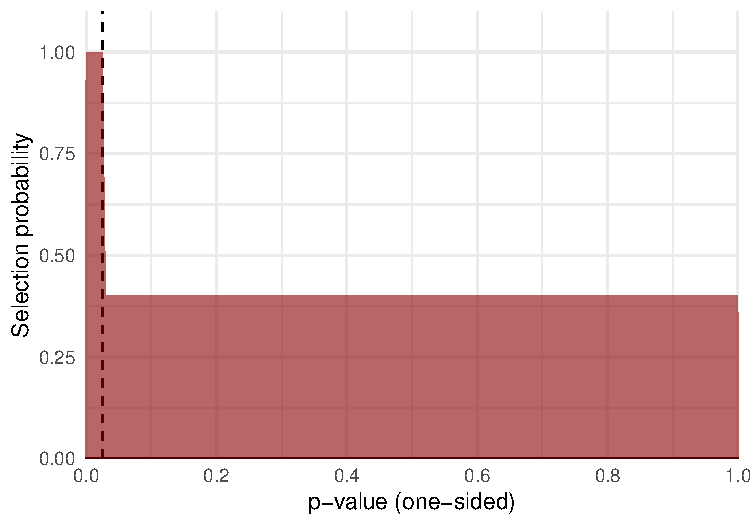
\includegraphics[width=0.49\linewidth]{selection_models_draft_files/figure-latex/step-functions-1} }\subfloat[Two-step selection with $\lambda_1 = 0.4, \lambda_2 = 0.2$\label{fig:step-functions-2}]{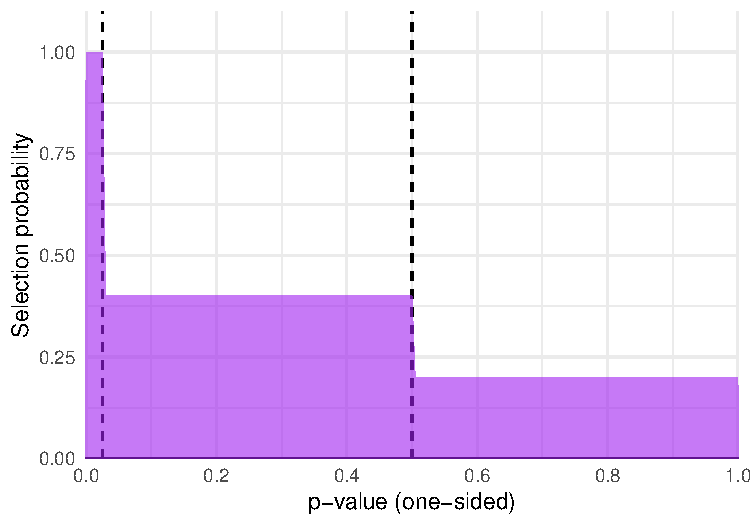
\includegraphics[width=0.49\linewidth]{selection_models_draft_files/figure-latex/step-functions-2} }\caption{Examples of step functions}\label{fig:step-functions}
\end{figure}

\subsection{Distribution of observed effect size estimates}\label{distribution-of-observed-effect-size-estimates}

Combining the assumptions of the evidence-generating process and the selection process leads to a model for an observed effect size estimate. The distribution of an observed effect size estimate is equivalent to the distribution of \(Y^*\) given that \(O = 1\). By Bayes rule,
\[
\Pr(Y^* = y | O = 1, \sigma^* = \sigma) = \frac{\Pr(O = 1 | Y^* = y, \sigma^* = \sigma) \times \Pr(Y^* = y | \sigma^* = \sigma)}{\Pr(O = 1 | \sigma^* = \sigma)},
\]
where the selection process defines the first term in the numerator and the evidence-generating process defines the second term in the numerator. The marginal density of an observed effect size estimate \(Y\) with standard error \(\sigma\) therefore has the form
\begin{equation}
\label{eq:generic-selection}
f(Y = y | \sigma, \mathbf{x}) = \frac{1}{A(\mathbf{x}, \sigma; \boldsymbol\beta, \tau^2, \boldsymbol\lambda)} \times w\left(y, \sigma; \boldsymbol\lambda \right) \times \frac{1}{\sqrt{\tau^2 + \sigma^2}} \phi\left(\frac{y - \mathbf{x} \boldsymbol\beta}{\sqrt{\tau^2 + \sigma^2}}\right),
\end{equation}
where
\begin{equation}
\label{eq:generic-selection-A}
A(\mathbf{x}, \sigma; \boldsymbol\beta, \tau^2, \boldsymbol\lambda) =  \int_\mathbb{R} w\left(y, \sigma; \boldsymbol\lambda \right) \times  \frac{1}{\sqrt{\tau^2 + \sigma^2}}\phi\left(\frac{y - \mathbf{x}\boldsymbol\beta}{\sqrt{\tau^2 + \sigma^2}}\right) dy.
\end{equation}
If \(w(y, \sigma; \boldsymbol\lambda) = 1\), then there is no selective reporting, \(A(\mathbf{x}, \sigma; \boldsymbol\beta, \tau^2, \boldsymbol\lambda) = 1\), and the density reduces to the unweighted density of the evidence-generating process (i.e., the density of a random-effects meta-regression).

For the step-function selection process, the \(A(\mathbf{x}, \sigma; \boldsymbol\beta, \tau^2, \boldsymbol\lambda)\) term in the step-function composite likelihood can be computed using the closed-form expression
\begin{equation}
\label{eq:step-function-A}
A_{ij} = A(\mathbf{x}_{ij}, \sigma_{ij}; \boldsymbol\beta, \tau^2, \boldsymbol\lambda) = \sum_{h=0}^H \lambda_h B_{hij}
\end{equation}
where
\begin{equation}
\label{eq:step-function-Bhij}
B_{hij} = \Phi\left(c_{hij}\right) - \Phi\left(c_{h+1,ij}\right),
\end{equation}
and \(c_{hij} = \left(\sigma_{ij} \Phi^{-1}\left(1 - \alpha_h\right) - \mathbf{x}_{ij}\boldsymbol\beta\right) / \sqrt{\tau^2 + \sigma_{ij}^2}\) for \(h = 0,...,H\) (Vevea \& Hedges, 1995).
The quantity \(B_{hij}\) corresponds to the probability that, prior to selection, a generated effect size estimate with predictor \(\mathbf{x}_{ij}\) and standard error \(\sigma_{ij}\) will have a p-value falling in the interval \(\alpha_h < p^* \leq \alpha_{h+1}\).

\subsection{Estimation Methods}\label{estimation-methods}

Past developments of selection models have focused either on maximum likelihood estimation under the assumption that all effect sizes are mutually independent (Citkowicz \& Vevea, 2017; Hedges, 1992; Vevea \& Hedges, 1995) or on sensitivity analysis methods that treat the selection model as known (Mathur \& VanderWeele, 2020; Vevea \& Woods, 2005). We consider several estimation and inference strategies that build upon and generalize past approaches, including maximum composite marginal likelihood and an alternative based on re-weighting the Gaussian likelihood of the evidence-generating process.
With both approaches, we allow for incorporation of prior weights.
Doing so permits inference based on the fractional random weight bootstrap (Xu et al., 2020), also known as the Bayesian bootstrap (Rubin, 1981), a technique that can be applied to estimation strategies that admit the use of weights.\footnote{Another reason to consider weights is that analytic weights could be used to improve the efficiency of the parameter estimators, similar to the working model weights proposed by Hedges et al. (2010) for random effects meta-analysis and meta-regression. For instance, consider the basic meta-analysis context with no predictors. If effect size estimates from the same study are correlated, then a study with \(k_j\) observed effect size estimates could contribute somewhat less than \(k_j\) independent pieces of information. Down-weighting the effect sizes from study \(j\) based on the number of reported effect sizes \(k_j\) might therefore improve the efficiency of the estimator for the average effect size \(\beta\) and variance \(\tau^2\).}
Thus, let \(a_{11},...,a_{J k_j}\) be a set of prior weights assigned to each study.

\subsubsection{Maximum composite marginal likelihood}\label{maximum-composite-marginal-likelihood}

Composite marginal likelihood techniques involve working with the marginal distribution of each observation (here, each observed effect size estimate) as if all observations were mutually independent (Cox \& Reid, 2004; Lindsay, 1988; Varin, 2008).
Thus, we assume that the observed effect size estimates were generated from Equation \eqref{eq:generic-selection}.
For purposes of estimation, we write the likelihoods using natural log transformations of the variance parameter and selection parameters, with \(\gamma = \log \tau^2\), \(\zeta_h = \log \lambda_h\), and \(\boldsymbol\zeta = \left[\zeta_1,...,\zeta_H\right]'\).
The log of the marginal likelihood contribution for effect size estimate \(i\) from study \(j\) is given by
\begin{align}
l^M_{ij}\left(\boldsymbol\beta, \gamma, \boldsymbol\zeta \right) &= \log f\left(Y = y_{ij} | \sigma_{ij}, \mathbf{x}_{ij}\right) \nonumber \\
&\propto \log w\left(y_{ij}, \sigma_{ij}; \boldsymbol\zeta \right) - \frac{1}{2} \frac{\left(y_{ij} - \mathbf{x}_{ij} \boldsymbol\beta\right)^2}{\exp(\gamma) + \sigma_{ij}^2} \nonumber\\
& \qquad \qquad  - \frac{1}{2}\log\left(\exp(\gamma) + \sigma_{ij}^2\right) - \log A\left(\mathbf{x}_{ij}, \sigma_{ij}; \boldsymbol\beta, \gamma, \boldsymbol\zeta \right). \label{eq:log-like-ij}
\end{align}
The weighted composite marginal log-likelihood across all \(J\) studies is then
\begin{equation}
\label{eq:marginal-likelihood}
l^M\left(\boldsymbol\beta, \gamma, \boldsymbol\zeta\right) = \sum_{j=1}^J \sum_{i=1}^{k_j} a_{ij} l^M_{ij}\left(\boldsymbol\beta, \gamma, \boldsymbol\zeta\right).
\end{equation}
The composite marginal likelihood (CML) estimators, denoted as \(\boldsymbol{\hat\beta}\), \(\hat\gamma\), and \(\boldsymbol{\hat\zeta}\), are obtained as the set of parameter values that maximize the composite likelihood for the observed data, as given in Equation (\ref{eq:marginal-likelihood}).

Under the assumption that the true parameter values are not at the extremes of their ranges, the CML estimator can also be defined as the solution of the weighted score equations,
\begin{equation}
\sum_{j=1}^J \mathbf{S}_{j}\left(\boldsymbol{\hat\beta}, \hat\gamma, \boldsymbol{\hat\zeta}\right) = \mathbf{0}
\end{equation}
where \(\mathbf{S}_j = \left(\mathbf{S}_{\boldsymbol\beta j}' \  S_{\gamma j} \ \mathbf{S}_{\boldsymbol\zeta j}'\right)'\) denotes the score vector from study \(j\), consisting of the derivatives of the likelihood contributions for each study with respect to the component parameters:
\begin{align}
\mathbf{S}_{\boldsymbol\beta j}\left(\boldsymbol{\beta}, \gamma, \boldsymbol{\zeta}\right) &= \sum_{i=1}^{k_j} a_{ij} \frac{\partial l^M_{ij}\left(\boldsymbol\beta, \gamma, \boldsymbol\zeta\right)}{\partial \boldsymbol\beta} \label{eq:score-M-beta} \\
S_{\gamma j}\left(\boldsymbol{\beta}, \gamma, \boldsymbol{\zeta}\right) &= \sum_{i=1}^{k_j} a_{ij} \frac{\partial l^M_{ij}\left(\boldsymbol\beta, \gamma, \boldsymbol\zeta\right)}{\partial \gamma} \label{eq:score-M-gamma} \\
\mathbf{S}_{\boldsymbol\zeta j}\left(\boldsymbol{\beta}, \gamma, \boldsymbol{\zeta}\right) &= \sum_{i=1}^{k_j} a_{ij} \frac{\partial l^M_{ij}\left(\boldsymbol\beta, \gamma, \boldsymbol\zeta\right)}{\partial \boldsymbol\zeta}. \label{eq:score-M-zeta} 
\end{align}
Appendix \ref{CML-derivatives} provides exact expressions for the score vectors of the step-function selection model.

Robust variance estimators, or sandwich estimators, are a commonly used technique for quantifying the uncertainty in CML estimators. Let \(\mathbf{H}\) denote the Hessian matrix of the composite log-likelihood,
\begin{equation}
\mathbf{H}(\boldsymbol\beta, \gamma, \boldsymbol\zeta) = \sum_{j=1}^J \frac{\partial \mathbf{S}_j(\boldsymbol\beta, \gamma, \boldsymbol\zeta)}{\partial \left(\boldsymbol\beta' \ \gamma \ \boldsymbol\zeta'\right)},
\end{equation}
exact expressions for which are given in Appendix \ref{CML-derivatives}.
Let \(\mathbf{\hat{S}}_j = \mathbf{S}_j(\boldsymbol{\hat\beta}, \hat\gamma, \boldsymbol{\hat\zeta})\) and \(\mathbf{\hat{H}} = \mathbf{H}(\boldsymbol{\hat\beta}, \hat\gamma, \boldsymbol{\hat\zeta})\) denote the score vectors and Hessian matrix evaluated at the maximum of the composite likelihood.
We then estimate the sampling variance of the CML estimator using a cluster-robust sandwich formula:
\begin{equation}
\label{eq:sandwich-variance}
\mathbf{V}^{CML} = \mathbf{\hat{H}}^{-1}\left(\sum_{j=1}^J \mathbf{\hat{S}}_j {\mathbf{\hat{S}}_j}'\right) \mathbf{\hat{H}}^{-1}.
\end{equation}
We construct confidence intervals for model parameters using \(\mathbf{V}^{CML}\) with Wald-type large sample approximations. For instance, the \((1 - 2\alpha)\)-level large-sample confidence interval for a meta-regression parameter \(\beta_g\) is constructed as
\[
\hat\beta_g \ \pm \ \Phi^{-1}(1 - \alpha) \times \sqrt{V^{CML}_{gg}},
\]
where \(V^{CML}_{gg}\) is the \(g^{th}\) diagonal entry of \(\mathbf{V}^{CML}\).

\subsubsection{Augmented, re-weighted Gaussian likelihood}\label{augmented-re-weighted-gaussian-likelihood}

Composite marginal likelihood is not the only possible basis for deriving estimators of selection model parameters.
In the framework of a sensitivity analysis for worst-case selection bias, Mathur and VanderWeele (2020) proposed using regular meta-analytic estimators for \(\boldsymbol\beta\), but with weights defined by the inverse probability of selection under a step-function selection model with a single step at \(\alpha_1 = .025\).
Because they were working in the context of sensitivity analysis, they assumed a maximum plausible degree of selection rather than estimating the parameters of a selection model, so that the weights were fixed and known quantities.
In contrast, here we will consider a more general model, possibly with multiple steps, using weights derived by estimating the selection model parameters.
We describe the estimators as augmented, re-weighted Gaussian likelihood (ARGL) estimators because the Gaussian likelihood of the evidence-generating process is re-weighted based on the selection process, with selection process parameters identified by augmenting the likelihood with an additional estimating equation.

Given the parameters of the selection process, we can calculate relative probabilities of selection for each effect size estimate, \(w_{ij} = w(y_{ij}, \sigma_{ij}; \boldsymbol\zeta)\). Following Mathur and VanderWeele (2020), we use these selection probabilities to form weighted estimating equations for the evidence-generating process. Under the evidence-generation model, the marginal log-likelihood of effect size estimate \(i\) from study \(j\) is Gaussian, given by
\[
l^G_{ij}(\boldsymbol\beta, \gamma) \propto - \frac{1}{2}\frac{(y_{ij} - \mathbf{x}_{ij} \boldsymbol\beta)^2}{\exp(\gamma) + \sigma_{ij}^2} - \frac{1}{2}\log(\exp(\gamma) + \sigma_{ij}^2).
\]
Allowing for prior weights, the inverse selection-weighted Gaussian log-likelihood is therefore
\[
l^G(\boldsymbol\beta, \gamma, \boldsymbol\zeta) = \sum_{j=1}^J \sum_{i=1}^{k_j} \frac{a_{ij}} {w_{ij}} \times l^G_{ij}(\boldsymbol\beta, \gamma).
\]
If the parameters of the selection process were known, we could find estimators for \(\boldsymbol\beta\) and \(\gamma\) by maximizing \(l^G(\boldsymbol\beta, \gamma, \boldsymbol\zeta)\) for a fixed value of \(\boldsymbol\zeta\).
Equivalently, we could find the estimators as the solutions to the weighted score equations
\begin{align}
\sum_{j=1}^J \mathbf{S}^G_{\boldsymbol\beta j} (\boldsymbol\beta, \gamma, \boldsymbol\zeta) &= 0 \label{eq:hybrid-score-beta} \\
\sum_{j=1}^J \mathbf{S}^G_{\gamma j} (\boldsymbol\beta, \gamma, \boldsymbol\zeta) &= 0, \label{eq:hybrid-score-gamma}
\end{align}
where the score contributions for study \(j\) are
\begin{align}
\mathbf{S}^G_{\boldsymbol\beta j} (\boldsymbol\beta, \gamma, \boldsymbol\zeta) &= \sum_{i=1}^{k_j} a_{ij} \times \mathbf{x}_{ij}' \frac{y_{ij} - \mathbf{x}_{ij} \boldsymbol\beta}{w_{ij} \left(\exp(\gamma) + \sigma_{ij}^2\right)} \\
\mathbf{S}^G_{\gamma j} (\boldsymbol\beta, \gamma, \boldsymbol\zeta) &= \sum_{i=1}^{k_j} a_{ij} \times \frac{\exp(\gamma)}{2 w_{ij}} \left(\frac{(y_{ij} -\mathbf{x}_{ij} \boldsymbol\beta)^2}{\left(\exp(\gamma) + \sigma_{ij}^2\right)^2} - \frac{1}{\exp(\gamma) + \sigma_{ij}^2}\right).
\end{align}
The question remains how to obtain an estimator for \(\boldsymbol\zeta\).

We propose to estimate \(\boldsymbol\zeta\) by augmenting the Gaussian log-likelihood with the marginal score equation with respect to \(\boldsymbol\zeta\).
Specifically, we define the ARGL estimators as the values that simultaneously solve Equations \eqref{eq:hybrid-score-beta} and \eqref{eq:hybrid-score-gamma} together with the estimating equation for \(\boldsymbol\zeta\) from the composite marginal likelihood approach.

With \(\mathbf{S}_{\boldsymbol\zeta j}\left(\boldsymbol{\beta}, \gamma, \boldsymbol{\zeta}\right)\) as given in Equation \eqref{eq:score-M-zeta}, the full set of estimating equations is
\begin{equation}
\label{eq:hybrid-score}
\mathbf{M}_j(\boldsymbol\beta, \gamma, \boldsymbol\zeta) = \left[\begin{array}{c} \mathbf{S}^G_{\boldsymbol\beta j}(\boldsymbol\beta, \gamma, \boldsymbol\zeta) \\ S^G_{\gamma j}(\boldsymbol\beta, \gamma, \boldsymbol\zeta) \\ \mathbf{S}_{\boldsymbol\zeta j}(\boldsymbol\beta, \gamma, \boldsymbol\zeta) \end{array}\right],
\end{equation}
based on which we define the ARGL estimator as the solution to the estimating equations
\begin{equation}
\label{eq:hybrid-total-score}
\sum_{j=1}^J \mathbf{M}_j(\boldsymbol\beta, \gamma, \boldsymbol\zeta) = \mathbf{0}.
\end{equation}
We will denote the ARGL parameter estimators as \(\boldsymbol{\tilde\beta}\), \(\tilde\gamma\), and \(\boldsymbol{\tilde\zeta}\).\footnote{For computational purposes, it is useful to observe that the solution to Equation \eqref{eq:hybrid-score-beta} involves a weighted least squares estimator for \(\boldsymbol\beta\). Given values of \(\gamma\) and \(\boldsymbol\zeta\), \(\boldsymbol{\tilde\beta}\) is
  \[
  \boldsymbol{\tilde\beta}(\gamma, \boldsymbol\zeta) = \left(\sum_{j=1}^J \sum_{i=1}^{k_j} v_{ij} \mathbf{x}_{ij}' \mathbf{x}_{ij}\right)^{-1} \sum_{j=1}^J \sum_{i=1}^{k_j} v_{ij} \mathbf{x}_{ij}' \mathbf{y}_{ij},
  \]
  where \(v_{ij} = \frac{a_j}{w_{ij} \left(\exp(\gamma) + \sigma_{ij}^2\right)}\).
  The weighted least squares solution allows \(\boldsymbol\beta\) to be profiled out of the estimating equations, so that Equation \eqref{eq:hybrid-total-score} need be solved only for \(\gamma\) and \(\boldsymbol\zeta\).}

For the step-function selection process, the score equation with respect to \(\boldsymbol\zeta\) has an interesting and intuitively intepretable form.
Observe that the probability that an observed effect size estimate with predictor \(\mathbf{x}_{ij}\) and standard error \(\sigma_{ij}\) will have a p-value falling in the interval \(\alpha_h < p^* \leq \alpha_{h+1}\) is \(E_{hij} = \exp(\zeta_h) \times B_{hij} / A_{ij}\), where \(B_{hij}\) is given in Equation \eqref{eq:step-function-Bhij}.
Accounting for the prior weights, the expected number of observed effect size estimates falling into the interval \((\alpha_h, \alpha_{h+1}]\) is therefore
\begin{equation}
\label{eq:expected-h}
E_h = \sum_{j=1}^J \sum_{i=1}^{k_j} a_{ij} \times \frac{\exp(\zeta_h) \times B_{hij}}{A_{ij}}.
\end{equation}
Let \(K_h = \sum_{j=1}^J \sum_{i=1}^{k_j} a_{ij} \times I\left(\alpha_h < p_{ij} \leq \alpha_{h+1}\right)\) denote the weighted count of observed effect size estimates with \(p\)-values falling into the interval \((\alpha_h, \alpha_{h+1}]\), for \(h = 0,...,H\).
The score of the step-function model with respect to the \(h^{th}\) component of \(\boldsymbol\zeta\) can then be written simply as
\begin{equation}
S_{\zeta h} = K_h - E_h.
\end{equation}
Thus, by setting \(\mathbf{S}_{\boldsymbol\zeta} = \mathbf{0}\), the estimator of \(\boldsymbol\zeta\) is taken to be the values that equate the observed number of effect size estimates in each interval with the expected number of estimates under the step-function model.

We will consider conducting inferences for the ARGL estimators using cluster-robust sandwich variance estimators that have the same form as (\ref{eq:sandwich-variance}).
Appendix \ref{ARGL-derivatives} provides further details.
We construct confidence intervals for model parameters using Wald-type large sample approximations, just as with the CML estimators.

\subsection{Bootstrap inference}\label{bootstrap-inference}

Sandwich estimators such as those in Equations \eqref{eq:sandwich-variance} require a large number of independent clusters (i.e., large \(J\)) to provide accurate assessments of uncertainty.
For regular meta-analysis or meta-regression models, small-sample refinements are available that provide accurate inference even with a limited number of clusters (Tipton, 2015; Tipton \& Pustejovsky, 2015).
However, these small-sample refinements have not been extended to step-function selection models.
We instead consider alternative inference techniques, including several forms of bootstrapping, that might provide more accurate inference with a limited number of clusters.
Bootstrap techniques involve generating many new pseudo-samples of observations by randomly perturbing the original sample, then re-calculating an estimator using each pseudo-sample.
The distribution of the estimator across pseudo-samples is used as a proxy for the actual sampling distribution of the estimator, providing a means to calculate standard errors and confidence intervals.

Many different bootstrap sampling schemes have been described that apply to different data structures and require different assumptions (Davison \& Hinkley, 1997).
For data involving dependent observations, it is crucial that the process used to generate pseudo-samples accounts for the dependence structure.
Techniques that do so include the non-parametric clustered bootstrap (also known as the clustered pairs bootstrap) and the fractional random weight bootstrap (Rubin, 1981; Xu et al., 2020).

In the non-parametric clustered bootstrap, each pseudo-sample is generated by randomly drawing \(J\) clusters of observations, with replacement, from the original sample.
Because clusters are drawn with replacement, some will necessarily be included multiple times and some clusters might not be included in a given pseudo-sample.
The process is equivalent to assigning a random set of weights to each cluster, where the weights for pseudo-sample \(b\) are drawn from a multinomial distribution with \(J\) trials and equal probability on each of \(J\) categories.

The fractional random weight bootstrap follows a very similar process in which each pseudo-sample is generated by assigning a random weight to every observation.
Rather than using a multinomial distribution, the weights follow independent exponential distributions with mean 1, so that the weights for pseudo-sample \(b\) are generated as \(a^{(b)}_j \sim Exp(1)\), with \(a_{ij}^{(b)} = a^{(b)}_j\) for \(i = 1,...,k_j\) and \(j = 1,...,J\).
A crucial difference between these bootstrap techniques is that the fractional random weight bootstrap puts strictly positive weight on every cluster of observations in every pseudo-sample, whereas the non-parametric bootstrap can assign zero weight to some clusters (Xu et al., 2020).
If the existence of an estimator hinges on the inclusion of one or a small number of clusters, this will create computational problems for the non-parametric bootstrap but not for the fractional random weight bootstrap.

For constructing confidence intervals, bootstrapping entails generating a total of \(B\) pseudo-samples, where \(B\) is a large number such as 1999, and re-calculating the estimator for each pseudo-sample.
There are several methods for constructing confidence intervals from a bootstrap distribution.
We consider four standard methods, all as described by Davison and Hinkley (1997), including the percentile CI, basic CI, studentized CI, and the bias-corrected-and-accelerated CI proposed by Efron (1987).
Appendix \ref{bootstrap-CIs} provides further details about the bootstrap CI calculations.

\section{Empirical Example}\label{empirical-example}

To demonstrate the proposed modeling strategy and examine potential differences between CML and ARGL estimation methods, we re-analyzed the data from a meta-analysis reported by Carter et al. (2015).
The meta-analyses examined a large corpus of primary studies on the ego depletion effect, which refers to the theory that an individual's ability to exercise self-control diminishes with repeated exertion (Hagger et al., 2010).
Carter et al. (2015) argued that the apparent strength of ego-depletion effects may be overstated due to selective reporting.
Their review included a variety of self-control manipulation tasks as well as a range of outcomes.
Some primary studies reported effects for multiple outcome tasks, leading to dependent effects.
Effect sizes were measured as standardized mean differences, defined so that positive effects correspond to depletion of self-control (i.e., consistent with the theory of ego depletion).

To mitigate possible effect of selective reporting, Carter et al. (2015) included many unpublished studies, so that the full meta-analysis included 116 effects from 66 studies.
For illustrative purposes, we re-analyzed the findings from the subset of published studies only; we also excluded a single outlying effect size estimate that was greater than 2. This analytic sample includes 66 effect size estimates from 45 distinct studies.
We conducted the analyses using R Version 4.4.3 (R Core Team, 2025).

If selective reporting were not a concern, a correlated-and-hierarchical effects model (CHE, Pustejovsky \& Tipton, 2022) would be one way to summarize the distribution of ego depletion effects.
Based on a CHE model, the overall average effect estimate was 0.46, 95\% CI {[}0.34, 0.59{]}.
Alternately, Chen and Pustejovsky (2024) proposed estimating average effect sizes using a CHE model with inverse sampling covariance weighting (CHE-ISCW), which does use the between-study or within-study variance estimates in forming weights. The CHE-ISCW estimator places relatively more weight on larger studies (those with smaller sampling variances), which are less biased by selective reporting.
Applying CHE-ISCW reduces the overall effect estimate to 0.39, 95\% CI {[}0.24, 0.54{]}.
As a further point of comparison, we estimated the overall average effect using the PET/PEESE regression adjustment (Stanley \& Doucouliagos, 2014), clustering the standard errors by study. This yielded an overall average effect of -0.09, 95\% CI {[}-0.76, 0.58{]}. The CHE and CHE-ISCW estimates are both positive, significant, and similar in magnitude. The PET-PEESE estimate is negative and much smaller than the CHE and CHE-ISCW estimates, indicating a pattern of small study effects.

We used the \texttt{selection\_model()} function from the \texttt{metaselection} package to fit single-step and two-step selection models (Pustejovsky \& Joshi, 2025).
The single-step model used a threshold at \(\alpha_1 = 0.025\); the two-step model used thresholds at \(\alpha_1 = 0.025\) and \(\alpha_2 = 0.5\).
For comparison purposes, we estimated model parameters using both CML and ARGL and computed cluster-robust and percentile bootstrap confidence intervals.
For bootstrapping, we used multinomial cluster bootstrap re-sampling with 1999 replicates.

\begin{table}
\centering
\caption{\label{tab:empirical}Single-step and two-step selection model parameter estimates fit to ego depletion effects data from Carter et al. (2015)}
\centering
\resizebox{\ifdim\width>\linewidth\linewidth\else\width\fi}{!}{
\begin{threeparttable}
\begin{tabular}[t]{l>{\raggedright\arraybackslash}p{5.5em}>{\raggedright\arraybackslash}p{5.5em}>{\raggedright\arraybackslash}p{5.5em}>{\raggedright\arraybackslash}p{5.5em}>{\raggedright\arraybackslash}p{5.5em}>{\raggedright\arraybackslash}p{5.5em}}
\toprule
\multicolumn{1}{c}{ } & \multicolumn{3}{c}{CML estimator} & \multicolumn{3}{c}{ARGL estimator} \\
\cmidrule(l{3pt}r{3pt}){2-4} \cmidrule(l{3pt}r{3pt}){5-7}
Parameter & Estimate (SE) & Cluster-Robust CI & Percentile Bootstrap CI & Estimate (SE) & Cluster-Robust CI & Percentile Bootstrap CI\\
\midrule
\addlinespace[0.3em]
\multicolumn{7}{l}{\textbf{One-step}}\\
\hspace{1em}$\beta$ & 0.25 (0.09) & {}[ 0.07,      0.44] & {}[ 0.08, 0.45] & 0.27 (0.07) & {}[ 0.14,      0.41] & {}[ 0.12, 0.46]\\
\hspace{1em}$\tau^2$ & 0.11 (0.04) & {}[ 0.06,      0.20] & {}[ 0.03, 0.18] & 0.11 (0.04) & {}[ 0.06,      0.21] & {}[ 0.02, 0.20]\\
\hspace{1em}$\lambda_1$ & 0.27 (0.14) & {}[ 0.10,      0.75] & {}[ 0.08, 0.76] & 0.30 (0.10) & {}[ 0.16,      0.56] & {}[ 0.06, 1.18]\\
\addlinespace[0.3em]
\multicolumn{7}{l}{\textbf{Two-step}}\\
\hspace{1em}$\beta$ & 0.23 (0.11) & {}[ 0.02,      0.44] & {}[ 0.03, 0.45] & 0.25 (1.45) & {}[-2.59,      3.10] & {}[-0.04, 0.53]\\
\hspace{1em}$\tau^2$ & 0.11 (0.04) & {}[ 0.06,      0.21] & {}[ 0.04, 0.18] & 0.12 (0.33) & {}[ 0.00,     32.00] & {}[ 0.01, 0.18]\\
\hspace{1em}$\lambda_1$ & 0.27 (0.14) & {}[ 0.10,      0.74] & {}[ 0.08, 0.75] & 0.29 (1.65) & {}[ 0.00,>100] & {}[ 0.05, 1.25]\\
\hspace{1em}$\lambda_2$ & 0.22 (0.16) & {}[ 0.06,      0.90] & {}[ 0.05, 0.96] & 0.26 (2.17) & {}[ 0.00,>100] & {}[ 0.01, 3.33]\\
\bottomrule
\end{tabular}
\begin{tablenotes}
\item \textit{Note: } 
\item ARGL = augmented, reweighted gaussian likelihood; CML = composite maximum likelihood; CI = confidence interval; SE = standard error.
\end{tablenotes}
\end{threeparttable}}
\end{table}

Table \ref{tab:empirical} presents the parameter estimates from the one-step and two-step selection models.
The estimated selection parameters are similar across the one- and two-step models and across both estimators, all indicating that non-significant or negative effect size estimates were less likely to be reported than statistically significant, affirmative ones.
The one-step and two-step selection model estimates of average effect size are positive but substantially smaller than the CHE-ISCW estimates, ranging from 0.23 to 0.27 depending on the model specification and estimation method.
In contrast to the PET/PEESE estimate, the selection model estimates using CML are positive and statistically distinct from zero.
Thus, an analyst would reach different conclusions about overall average effect size depending on whether they use an unadjusted model, a step-function model, or the PET/PEESE adjustment.

The estimates in Table \ref{tab:empirical} point towards some potential differences between estimation methods.
Generally, the CML and ARGL parameter estimates are similar in magnitude, but the confidence intervals based on the CML estimator are narrower than those for the ARGL estimator.
For the CML estimator, the bootstrap CIs are similar or slightly wider than the cluster-robust CIs.
For the ARGL estimator, the bootstrap CIs were similar to the cluster-robust CIs for the one-step model but quite discrepant for the two-step model.
For the two-step model, the cluster-robust CIs were so wide as to be entirely uninformative, whereas the bootstrap CIs were not as extreme.

The patterns that we have noted suggest that there could be differences in the performance of the estimators, as well as differences in performance between the step-function estimators and alternative adjustment methods such as PET/PEESE.
However, these results are based on a single empirical dataset where the true data-generating process is uncertain.
To draw firmer conclusion about the comparative performance of these methods, we conducted simulations to evaluate the methods in terms of bias, accuracy, and confidence interval coverage across a range of conditions.

\section{Simulation Methods}\label{simulation-methods}

We conducted Monte Carlo simulation studies to examine the performance
of the CML and ARGL estimators for a step-function selection model with a single step, under a wide range of conditions where primary studies contribute multiple, statistically dependent effect size estimates.
We compare the performance of these novel estimators to two available alternatives: a summary meta-analysis that addresses the dependency structure but does not correct for selective reporting and the PET-PEESE adjustment (Stanley \& Doucouliagos, 2014), a commonly used method for correcting selective reporting that has been adapted to handle dependent effects.
We evaluated the point estimators and robust variance estimators in terms of convergence rates, bias, accuracy, and confidence interval coverage for recovering the average effect size of the unselected distribution.
To limit the computational burden, we evaluated the performance of bootstrap confidence intervals across a more limited range of conditions.
We ran the simulation in R Version 4.4.1
(R Core Team, 2025) using the high-throughput computing cluster at the University of Wisconsin - Madison (Center for High Throughput Computing, 2006).
The simulation code drew on functionality from several R packages, including \texttt{metafor} (Viechtbauer, 2010), \texttt{clubSandwich} (Pustejovsky, 2024), \texttt{simhelpers} (Joshi \& Pustejovsky, 2024), \texttt{optimx} (Nash \& Varadhan, 2011), \texttt{nleqslv} (Hasselman, 2023), and \texttt{tidyverse} (Wickham et al., 2019).

\subsection{Data generation}\label{data-generation}

We simulated meta-analyses based on a CHE working model, with individual effect size estimates selected
for inclusion based on the step-function selection model with a single step at \(\alpha_1 = .025\).
For each replication, we generated a total of \(J^*\) studies with a two-group comparison
design, where study \(j\) contributed \(k_j^* \geq 1\) effect size estimates prior to selective reporting. Let
\(T_{ij}\) denote effect size estimate \(i\) from study \(j\) and let \(\sigma_{ij}\)
denote its standard error, for \(i = 1,...,k_j^*\) and \(j = 1,...,J^*\). Let \(N_j\)
denote the effective sample size from study \(j\).

To generate each meta-analytic dataset, we sampled effective sample sizes and numbers of effect sizes per study from an empirical distribution based on the What Works Clearinghouse database.
The total effective sample size per study was divided equally into two groups, treatment and control.
We then generated \(r_j\), an outcome correlation for study \(j\), by drawing from a beta distribution with mean \(\rho\) and standard deviation 0.05.
We assumed constant correlation between pairs of outcomes within a study but allowed the correlation to vary from study to study.

We then simulated raw outcomes for each primary study included in the
meta-analytic dataset. To do so, we first generated an average effect
size per study, \(\delta_j\), from a normal distribution with mean \(\mu\) and variance
of \(\tau^2\). Given \(\delta_j\), we generated \(k_j^*\) effect size parameters per study, \(\boldsymbol\delta_j = \left(\delta_{1j},...,\delta_{k_j^* j}\right)'\), from a normal distribution with mean of \(\delta_j\) and
variance of \(\omega^2\).
For each of the \(N_j / 2\) participants in the treatment and control groups, we then simulated vectors of multivariate normal outcomes as
\[
\mathbf{Y}_{hj}^T \sim N(\boldsymbol\delta_j, \boldsymbol\Psi_j) \qquad \text{and} \qquad
\mathbf{Y}_{hj}^C \sim N(\mathbf{0}, \boldsymbol\Psi_j).
\]
Here, \(\mathbf{Y}_{hj}^T\) and \(\mathbf{Y}_{hj}^C\) are
\(k_j^* \times 1\) vectors of outcomes for participant \(h\) in study \(j\) in
treatment and control group and \(\boldsymbol\Psi_j\) is the covariance matrix for outcomes in study \(j\), with the diagonal elements equal to 1 and off-diagonal elements equal to \(r_j\).
From the raw outcome data, we calculated standardized mean
differences using Hedges's \(g\) bias correction for each of the correlated outcomes, yielding effect size estimates \(y^*_{ij}\) for \(i=1,...,k_j^*\) and \(j = 1,...,J^*\).
We calculated the sampling variances using conventional formulas (Borenstein \& Hedges, 2019) and computed one-sided \(p\)-values based on two-sample \(t\)-tests for the null of \(H_0: \delta_{ij} \leq 0\).

After simulating results for study \(j\), we applied a step-function selection
model to the individual effect size estimates, with a one-sided selection
threshold at \(\alpha = 0.025\). Specifically, we let result \((y^*_{ij},
\sigma_{ij}^*, p_{ij}^*)\) be included in the observed dataset with probability
1 if \(p_{ij}^*\) was less than 0.025 and with probability \(0 < \lambda_1 \leq 1\) if \(p_{ij}^* \ge 0.025\).
We repeated the process of generating studies until the database included a total of \(J\) studies with at least one observed result, where observed study \(j\) includes \(k_j\) effect size estimates for \(1 \leq k_j \leq k_j^*\).

\subsection{Estimation methods}\label{estimation-methods-1}

We estimated step-function selection models with a single step at \(\alpha_1 = 0.025\), so that the assumed marginal selection process is consistent with the actual selective reporting process used to generate meta-analytic datasets.
We estimated CML and ARGL estimators as described in Section \ref{estimation-methods}.
For both estimators, we calculated cluster-robust standard errors using large-sample sandwich formulas.
For a subset of simulation conditions, we also examined percentile, basic, studentized, and bias-corrected-and-accelerated bootstrap confidence intervals based on the non-parametric clustered bootstrap and the fractional random weight bootstrap.
To maintain computational feasibility, we used \(B = 399\) bootstrap replications of each estimator.

We compared the performance of the step-function CML and ARGL estimators to two alternative methods.
First, we estimated a summary meta-analysis model without any correction for selective reporting, using a method that accounts for effect size dependency.
Specifically, we used the CHE working model with inverse sampling-covariance weights (CHE-ISCW) as proposed by Chen and Pustejovsky (2024).
This approach uses the working model
\begin{equation}
\label{eq:che}
y_{ij} = \mu + u_j + v_{ij} + e_{ij},
\end{equation}
where \(u_j \sim N(0, \tau^2)\), \(v_{ij} \sim N(0, \omega^2)\), and \(e_{ij} \sim N(0, \sigma_{ij}^2)\).
We estimated the variance components \(\tau^2\) and \(\omega^2\) using restricted maximum likelihood, treating the sample variances \(\sigma_{ij}\) as known.
We assumed \(\text{cor}(e_{hj},e_{ij} )=0.80\) for all pairs of effect size estimates from the same study, which leads to a
degree of mis-specification when the average correlation used in the data-generating process differs from 0.80.
Rather than estimating \(\mu\) using weights based on the full working model, CHE-ISCW instead uses generalized least squares with weighting matrices that are the inverse of the variance-covariance matrix of the sampling errors \(e_{1j},...,e_{k_j j}\) only.
This has the effect of allocating more weight to studies with smaller sampling variances, providing some robustness to selective reporting of study results.
For this estimator, we calculated confidence intervals using cluster-robust variance estimation with the CR2 small-sample correction and Satterthwaite degrees of freedom.

Second, we implemented a variation of the PET/PEESE estimator originally proposed by Stanley and Doucouliagos (2014), adapted to
accommodate dependent effect sizes. The PET estimator is based on the
working model \begin{equation}
\label{eq:pet}
T_{ij} = \mu + \beta \times \frac{2}{\sqrt{N_j}} + e_{ij}
\end{equation} The PEESE estimator is similar, but uses the sampling
variance instead of the sampling standard error: \begin{equation}
\label{eq:peese}
T_{ij} = \mu + \beta \times \frac{4}{N_j} + e_{ij}
\end{equation} For both estimating equations, we assumed
\(e_{ij} \sim N(0, \sigma_{ij}^2)\) and \(\text{cor}(e_{hj},e_{ij} )=0.80\) and
estimated the model just as with the CHE-ISCW model, including using
CR2 cluster-robust standard errors. Following Stanley and Doucouliagos (2014), we combined
the estimators by using PEESE if the PET estimator is statistically
distinct from zero at an \(\alpha\)-level of 0.10, and otherwise using PET.

\subsection{Experimental design}\label{experimental-design}

Table \ref{tab:sim-design} summarizes the experimental design for this study.
Manipulated parameters included overall average standardized mean difference
(\(\mu\)), between-study heterogeneity (\(\tau\)), within-study heterogeneity ratio
(\(\omega^2 / \tau^2\)), average correlation between outcomes (\(\rho\)),
probability of selection for non-affirmative results (\(\lambda_1\)), number of observed studies (\(J\)), and primary study sample size.
Parameters were fully crossed for a total of \(4 \times 4 \times 2 \times 2 \times 6 \times 5 \times 2 = 3,840\) conditions in the full simulation study.
Due to the computational demands of bootstrapping, we focused the bootstrap simulations on conditions with a smaller number of studies, for which we expected large-sample cluster-robust CIs to be relatively less effective.
We also reduced the number of parameter values for factors where we did
not observe much variation in results in the full simulation
(e.g., \(\tau = 0.30\)).
This resulted in \(4 \times 2 \times 2 \times 1 \times 3 \times 3 \times 2 = 288\) conditions for the bootstrap simulations.
For each condition, we generated 2,000 replications.

\begin{table}
\centering
\caption{\label{tab:sim-design}Parameter values examined in the simulation study}
\centering
\begin{tabular}[t]{>{\raggedright\arraybackslash}p{2.5in}ll}
\toprule
Parameter & Full Simulation & Bootstrap Simulation\\
\midrule
Overall average SMD ($\mu$) & 0.0, 0.20, 0.40, 0.80 & 0, 0.2, 0.40, 0.80\\
Between-study heterogeneity ($\tau$) & 0.05, 0.15, 0.30, 0.45 & 0.15, 0.45\\
Heterogeneity ratio ($\omega^2 / \tau^2$) & 0.0, 0.50 & 0.0, 0.50\\
Average correlation between outcomes ($\rho$) & 0.40, 0.80 & 0.80\\
Probability of selection for non-affirmative effects ($\lambda_1$) & 0.02, 0.05, 0.10, 0.20, 0.50, 1.0 & 0.05, 0.20, 1.0\\
\addlinespace
Number of observed studies ($J$) & 15, 30, 60, 90, 120 & 15, 30, 60\\
Primary study sample size & Typical, Small & Typical, Small\\
\bottomrule
\end{tabular}
\end{table}

In the full simulation, we examined values for the overall average SMD (\(\mu\)) ranging from 0.0 to 0.80, which covers the range of effects observed in a review of 747 randomized control trials of education interventions by Kraft (2020).
We used values of \(\tau\) ranging from 0.05 (a very small degree of heterogeneity) to 0.45 (a large degree of heterogeneity).
We specified the degree of within-study heterogeneity in relative terms, by setting the ratio of \(\omega^2\) to between-study heterogeneity \(\tau^2\) at either 0 (i.e., no within-study heterogeneity) or 0.5.

For the average correlation between outcomes from the same study, we
examined the values of 0.40 or 0.80. The default value of the average
correlation in software packages that implement RVE is 0.80. Thus, in
conditions where \(\rho\) is 0.80, the working model is approximately
correctly specified. We included conditions where \(\rho = 0.4\) to examine performance when the
working model is not correctly specified.

We examined a wide range of values for the probability of selection for non-affirmative effect sizes, ranging from no selective reporting (\(\lambda_1 = 1\)) to very severe selective reporting \((\lambda_1 = 0.02)\).

We examined a wide range of conditions for the number of primary studies included in the meta-analysis, ranging from relatively small databases of \(J = 15\) to very large databases with \(J = 120\) studies.
We chose these values to cover the conditions found in real meta-analyses of education and psychology research (Tipton et al., 2019).

Lastly, we investigated the primary study sample size.
For the typical primary study sample sizes, we used the empirical distribution of sample sizes in the What Works Clearinghouse database of findings from educational intervention studies.
The sample sizes in the database ranged from 37 to 2,295 with a median of 211.
The number of effect sizes ranged from 1 to 48 with a median of 3.
To explore the influence of the effective sample size distribution, we also ran conditions in which we divided the sample
sizes from the What Works Clearinghouse database by three to represent primary studies with smaller sample sizes,
such as those used in psychology laboratory studies.

\subsection{Performance criteria}\label{performance-criteria}

We evaluated the performance of these methods in terms of convergence rates, bias,
scaled root mean-squared error (RMSE), and 95\% confidence interval coverage for the overall average effect size \(\mu\).
Bias measures whether an estimator generates values that are systematically (on average) above or below
the true parameter.
RMSE measures the overall accuracy of an estimator, capturing both systematic bias and sampling variance.
Because we expected that RMSE would decrease proportionally with the square-root of the number of studies, we scaled the RMSE of each estimator by \(\sqrt{J}\) to reduce variation across the number of studies included in each meta-analysis.
Because the sampling distribution of the CML and ARGL estimators sometimes included extreme outlying values, we calculated bias and scaled RMSE after winsorizing the distribution.
Specifically, we defined a lower fence of 2.5 times the inter-quartile range below the 25th percentile and an upper fence of 2.5 times the inter-quartile range above the 75th percentile.
Estimates falling below the lower fence or above the upper fence were set to the corresponding fence values.

For confidence intervals based on cluster-robust variance estimation, we calculated coverage rates as the proportion of simulated intervals that included the true parameter.
For bootstrap confidence intervals, estimation of coverage rates is complicated by the fact that coverage is affected by the number of bootstrap replications.
Due to the computational demands of bootstrapping, we used \(B = 399\) bootstraps per replication---fewer than recommended for analysis of real data.
To estimate coverage rates for confidence intervals as would be used in practice, we used an extrapolation technique similar to one proposed by Boos and Zhang (2000).
For each replication, we computed bootstrap confidence intervals not only for \(B = 399\), but also for \(B = 49\), 99, 199, and 299 bootstraps, randomly selected without replacement from the full set of \(B = 399\) bootstraps.
We computed coverage rates separately for each value of \(B\) and fit a linear regression of the coverage rate on \(1 / B\).
We used the intercept from this regression as the predicted coverage rate of confidence intervals based on \(B = 1999\) bootstraps.

\section{Simulation Results}\label{simulation-results}

We organize our presentation of simulation study results by first considering the properties of point and interval estimators for the average effect size.
For this parameter, we compare the bias and accuracy of the CML and ARGL estimators to that of the CHE-ISCW estimator and the PET/PEESE estimator.
We also examine the calibration of cluster-robust and bootstrap confidence intervals based on the CML and ARGL estimators.
We then briefly consider the bias and accuracy of estimators of the marginal variance of the effect size distribution and the selection parameter in the step-function model.

\subsection{Average Effect Size}\label{average-effect-size}

The CHE-ISCW and PET/PEESE estimators produced results for every replication in every condition.
The CML and ARGL estimators for the step-function selection model had very high convergence rates across most conditions, although the CML estimator did exhibit rates of convergence below 99\% under conditions with the lowest degree of heterogeneity \(\tau = 0.05\), with the lowest convergence rate of 94.40\%.
For the ARGL estimator, convergence was above 99.80\% across all conditions.
Supplementary Figure \ref{fig:convergence-rates} depicts the range of convergence rates of the CML and ARGL estimators.
We evaluated the performance characteristics of these estimators across replications where they converged.

\subsubsection{Bias}\label{bias}

\begin{sidewaysfigure}
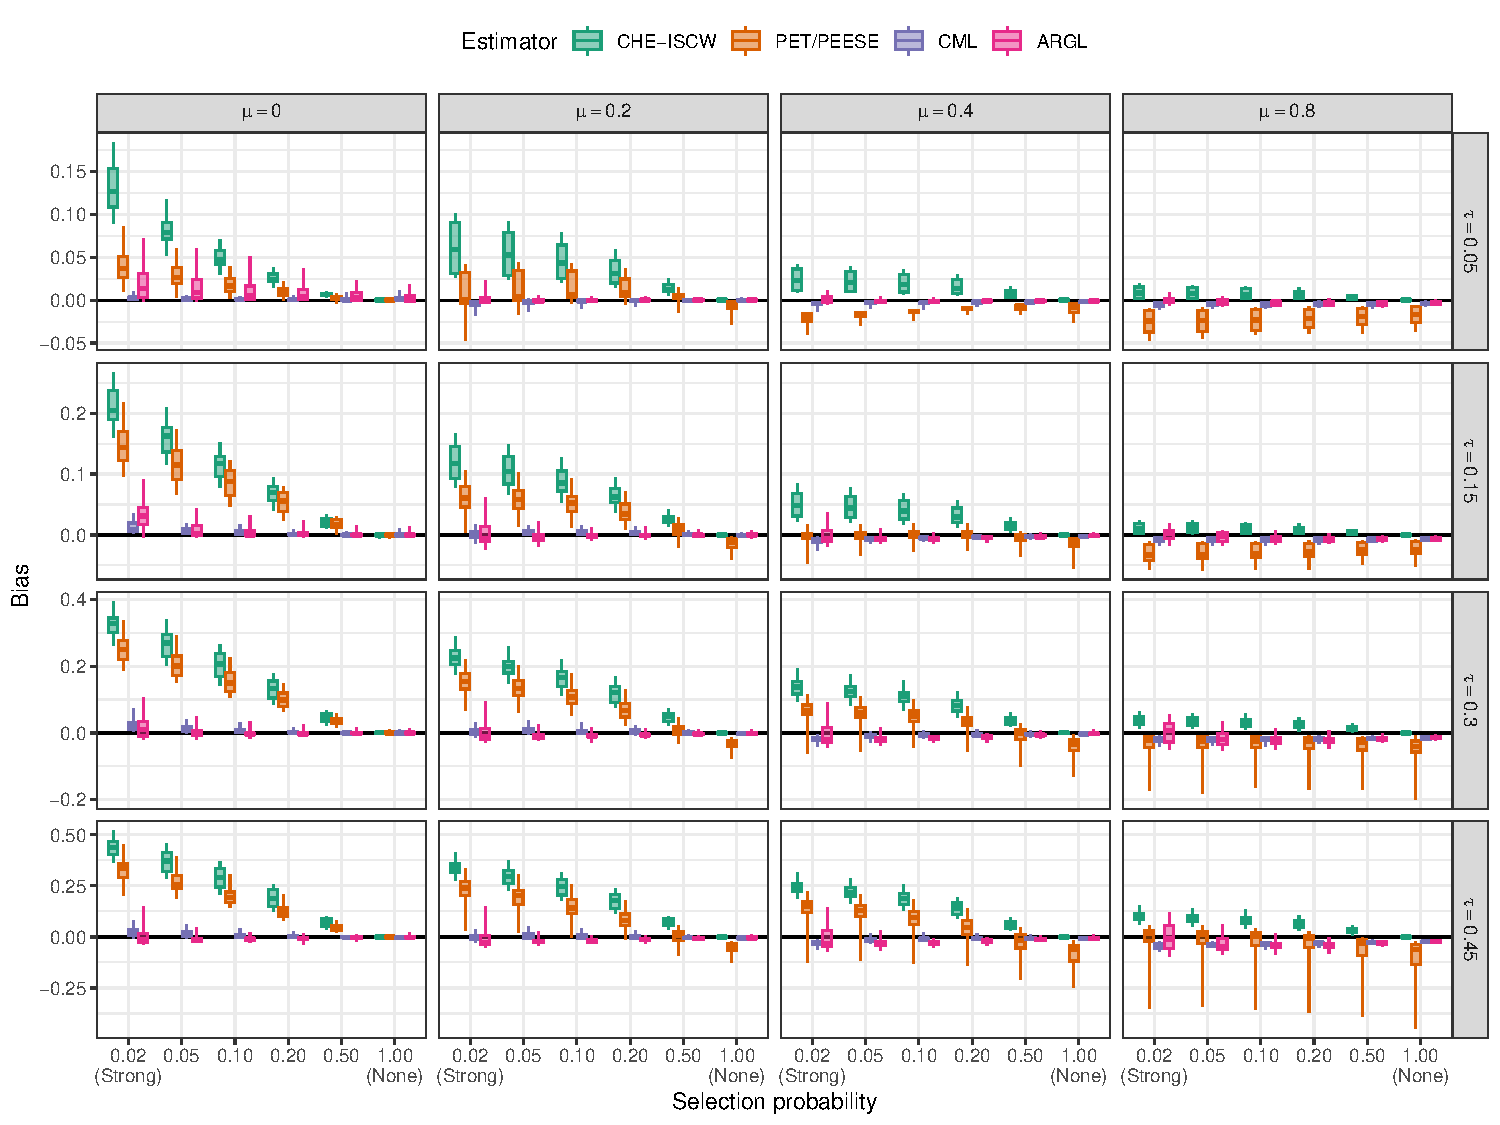
\includegraphics{selection_models_draft_files/figure-latex/mu-bias-1} \caption{Bias for estimators of average effect size by selection probability, average SMD, and between-study heterogeneity}\label{fig:mu-bias}
\end{sidewaysfigure}

Figure \ref{fig:mu-bias} depicts the bias (represented on the vertical axis of each plot) of each estimator of average effect size as a function of the strength of selective reporting (represented on the horizontal axis of each plot), average effect size parameter (varying by grid column), and between-study heterogeneity (\(\tau\), varying by grid row).
The box plot for each estimator depicts variation in bias over the remaining factors in the simulation design.
Note that the range of the vertical axis differs by grid row because the bias of some estimators is strongly influenced by the degree of heterogeneity.

The CML estimator has negligible or small bias across all conditions.
Its largest bias was 0.08, occurring when selective reporting is very strong, average effect size is zero, and heterogeneity is large.
The small bias of the CML estimator is stable across varying degrees of outcome correlation, within-study heterogeneity, number of observed studies, and primary study sample size.
Similar to the CML estimator, the ARGL estimator also has negligible or small bias across most conditions, although it becomes biased when average effect is zero and selection is very strong.

In contrast to the estimators based on the marginal selection model, the comparison estimators are systematically biased under many conditions.
The CHE-ISCW estimator, which does not directly adjust for selective reporting, is systematically biased under conditions with non-null selection.
When average effect size is large \((\mu = 0.8)\), its bias remains quite small even when selective reporting is very strong.
However, the bias of CHE-ISCW grows stronger when selection is more extreme, when average effect size is smaller, and when heterogeneity is larger, exceeding 0.50 when \(\mu = 0.0\), \(\tau = 0.45\), and \(\lambda_1 = 0.02\).
Although the PET/PEESE estimator uses a regression adjustment to account for possible selective reporting, it too becomes severely biased when selective reporting is strong.
For smaller values of average effect size \((\mu \leq 0.2)\), the bias of PET/PEESE tracks the bias of the CHE-ISCW estimator but is somewhat less pronounced; its bias grows stronger for smaller values of average effect size and higher levels of heterogeneity.
For larger values of average effect size \((\mu = 0.8)\), the PET/PEESE estimator is negatively biased---especially at high levels of heterogeneity.

\subsubsection{Scaled RMSE}\label{scaled-rmse}

\begin{sidewaysfigure}
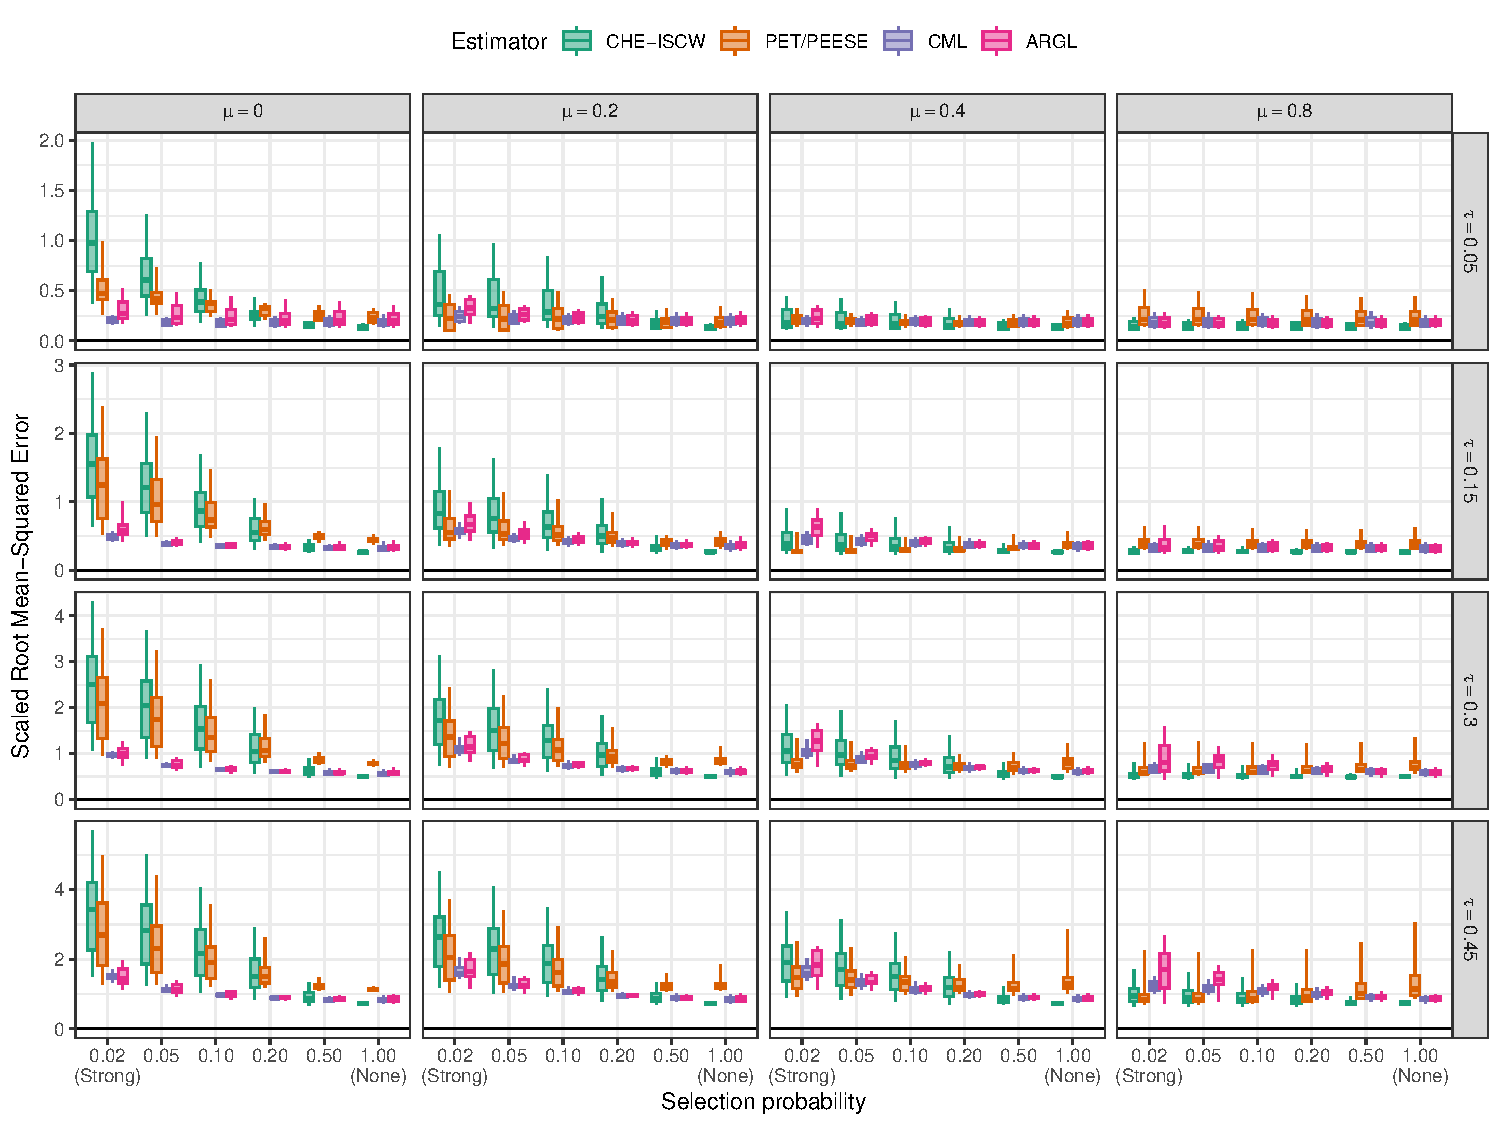
\includegraphics{selection_models_draft_files/figure-latex/mu-rmse-1} \caption{Scaled root mean-squared error for estimators of average effect size by selection probability, average SMD, and between-study heterogeneity}\label{fig:mu-rmse}
\end{sidewaysfigure}

Scaled RMSE combines both bias and variability into an overall measure of inaccuracy.
Figure \ref{fig:mu-rmse} depicts the scaled RMSE of each estimator of average effect size; it is constructed in the same way as Figure \ref{fig:mu-bias}.
Figures \ref{fig:rmse-ARGL-CML} through \ref{fig:rmse-PET-ARGL} in Appendix \ref{mu-simulation-results} provide greater detail about the relative accuracy of the four methods by plotting the ratio of RMSEs for each pair of methods.
These figures illustrate several findings.

First, across most data-generating conditions, the ARGL estimator has higher RMSE than the CML estimator. (This is evident in Figure \ref{fig:rmse-ARGL-CML}, which shows that that the RMSE ratio comparing ARGL to CML is greater than one across most conditions examined.)
The ARGL estimator has lower RMSE only under conditions of very high heterogeneity and in databases with few studies.
Thus, the CML will typically be preferable to the ARGL estimator.

Second, considering both the selection model estimators and comparison methods, no single method achieves the lowest RMSE uniformly across all conditions examined.
Instead, all methods face bias-variance trade-offs.
Under conditions with small or moderate average effect size and moderate or strong selection, the selection model estimators generally have lower RMSE than the CHE-ISCW and PET/PEESE estimators.
The CML estimator has lower RMSE than CHE-ISCW under most conditions where selective reporting creates meaningful bias---specifically, for \(\lambda_1 <= 0.2\) and \(\mu \leq 0.2\) (Figure \ref{fig:rmse-CHE-CML}).
The relative accuracy of the ARGL estimator versus CHE-ISCW follows a similar pattern (Figure \ref{fig:rmse-CHE-ARGL}).

Third, the CML estimator also has lower RMSE than PET/PEESE under conditions where where selective reporting creates meaningful bias, although it is not uniformly more accurate than PET/PEESE (Figure \ref{fig:rmse-PET-CML}).
Rather, PET/PEESE is more accurate under \emph{some} conditions involving moderate or large effect size \((\mu \geq 0.4)\) and varying degrees of between-study heterogeneity,
which correspond to conditions where the bias of PET/PEESE is small.
The relative accuracy is difficult to characterize generally because it follows a non-linear pattern involving interactions among the data-generating parameters.
The pattern of relative accuracy is very similar for the ARGL estimator (Figure \ref{fig:rmse-PET-ARGL}).

The bias-variance trade-offs faced by all the estimators arise because the CHE-ISCW estimator (which does not directly adjust for selection) is substantially biased by selective reporting, whereas the CML and ARGL estimators have at most small biases.
However, under conditions where selection is absent or small and where average effect size is larger, the CHE-ISCW estimator has greater precision than the estimators that adjust for selective reporting.
Because selective reporting does not create much bias under such conditions, the additional variability that comes with estimating a selection model or PET/PEESE adjustment dominates the small reduction in bias that these methods provide.

\subsubsection{Confidence Interval Coverage}\label{confidence-interval-coverage}

Figure \ref{fig:comparison-coverage} shows the coverage rates of 95\% CIs based on large-sample cluster-robust variance estimators for the CHE-ISCW, PET/PEESE, CML, and ARGL estimators.\footnote{To provide greater detail, the vertical axis of Figure \ref{fig:comparison-coverage} is limited to the range {[}0.5, 1.0{]}, and coverage rates of the CHE-ISCW and PET/PEESE intervals are not depicted when they fall below 0.5. Supplementary Figure \ref{fig:comparison-coverage-full} depicts the full range of coverage rates.}
Coverage rates are below the nominal rate of 0.95 for all methods across most conditions.
The CML and ARGL estimators based on the step-function selection model have higher coverage rates than the comparison methods under many conditions, particularly in conditions with higher between-study heterogeneity,\\
Intervals based on the CML and ARGL estimators have coverage levels that improve towards 0.95 as the number of studies increases, but are often still unacceptably low even when \(J = 90\) or greater.
In contrast, intervals based on CHE-ISCW and PET/PEESE are often wildly mis-calibrated due to the biases of these estimators.
Under conditions where CHE-ISCW and PET/PEESE are biased by selective reporting, their confidence intervals do not center on the true parameter. Consequently, as the number of studies increases, the standard error of the estimators decreases (as does the width of confidence intervals) and their coverage rates degrade towards zero.

\begin{sidewaysfigure}
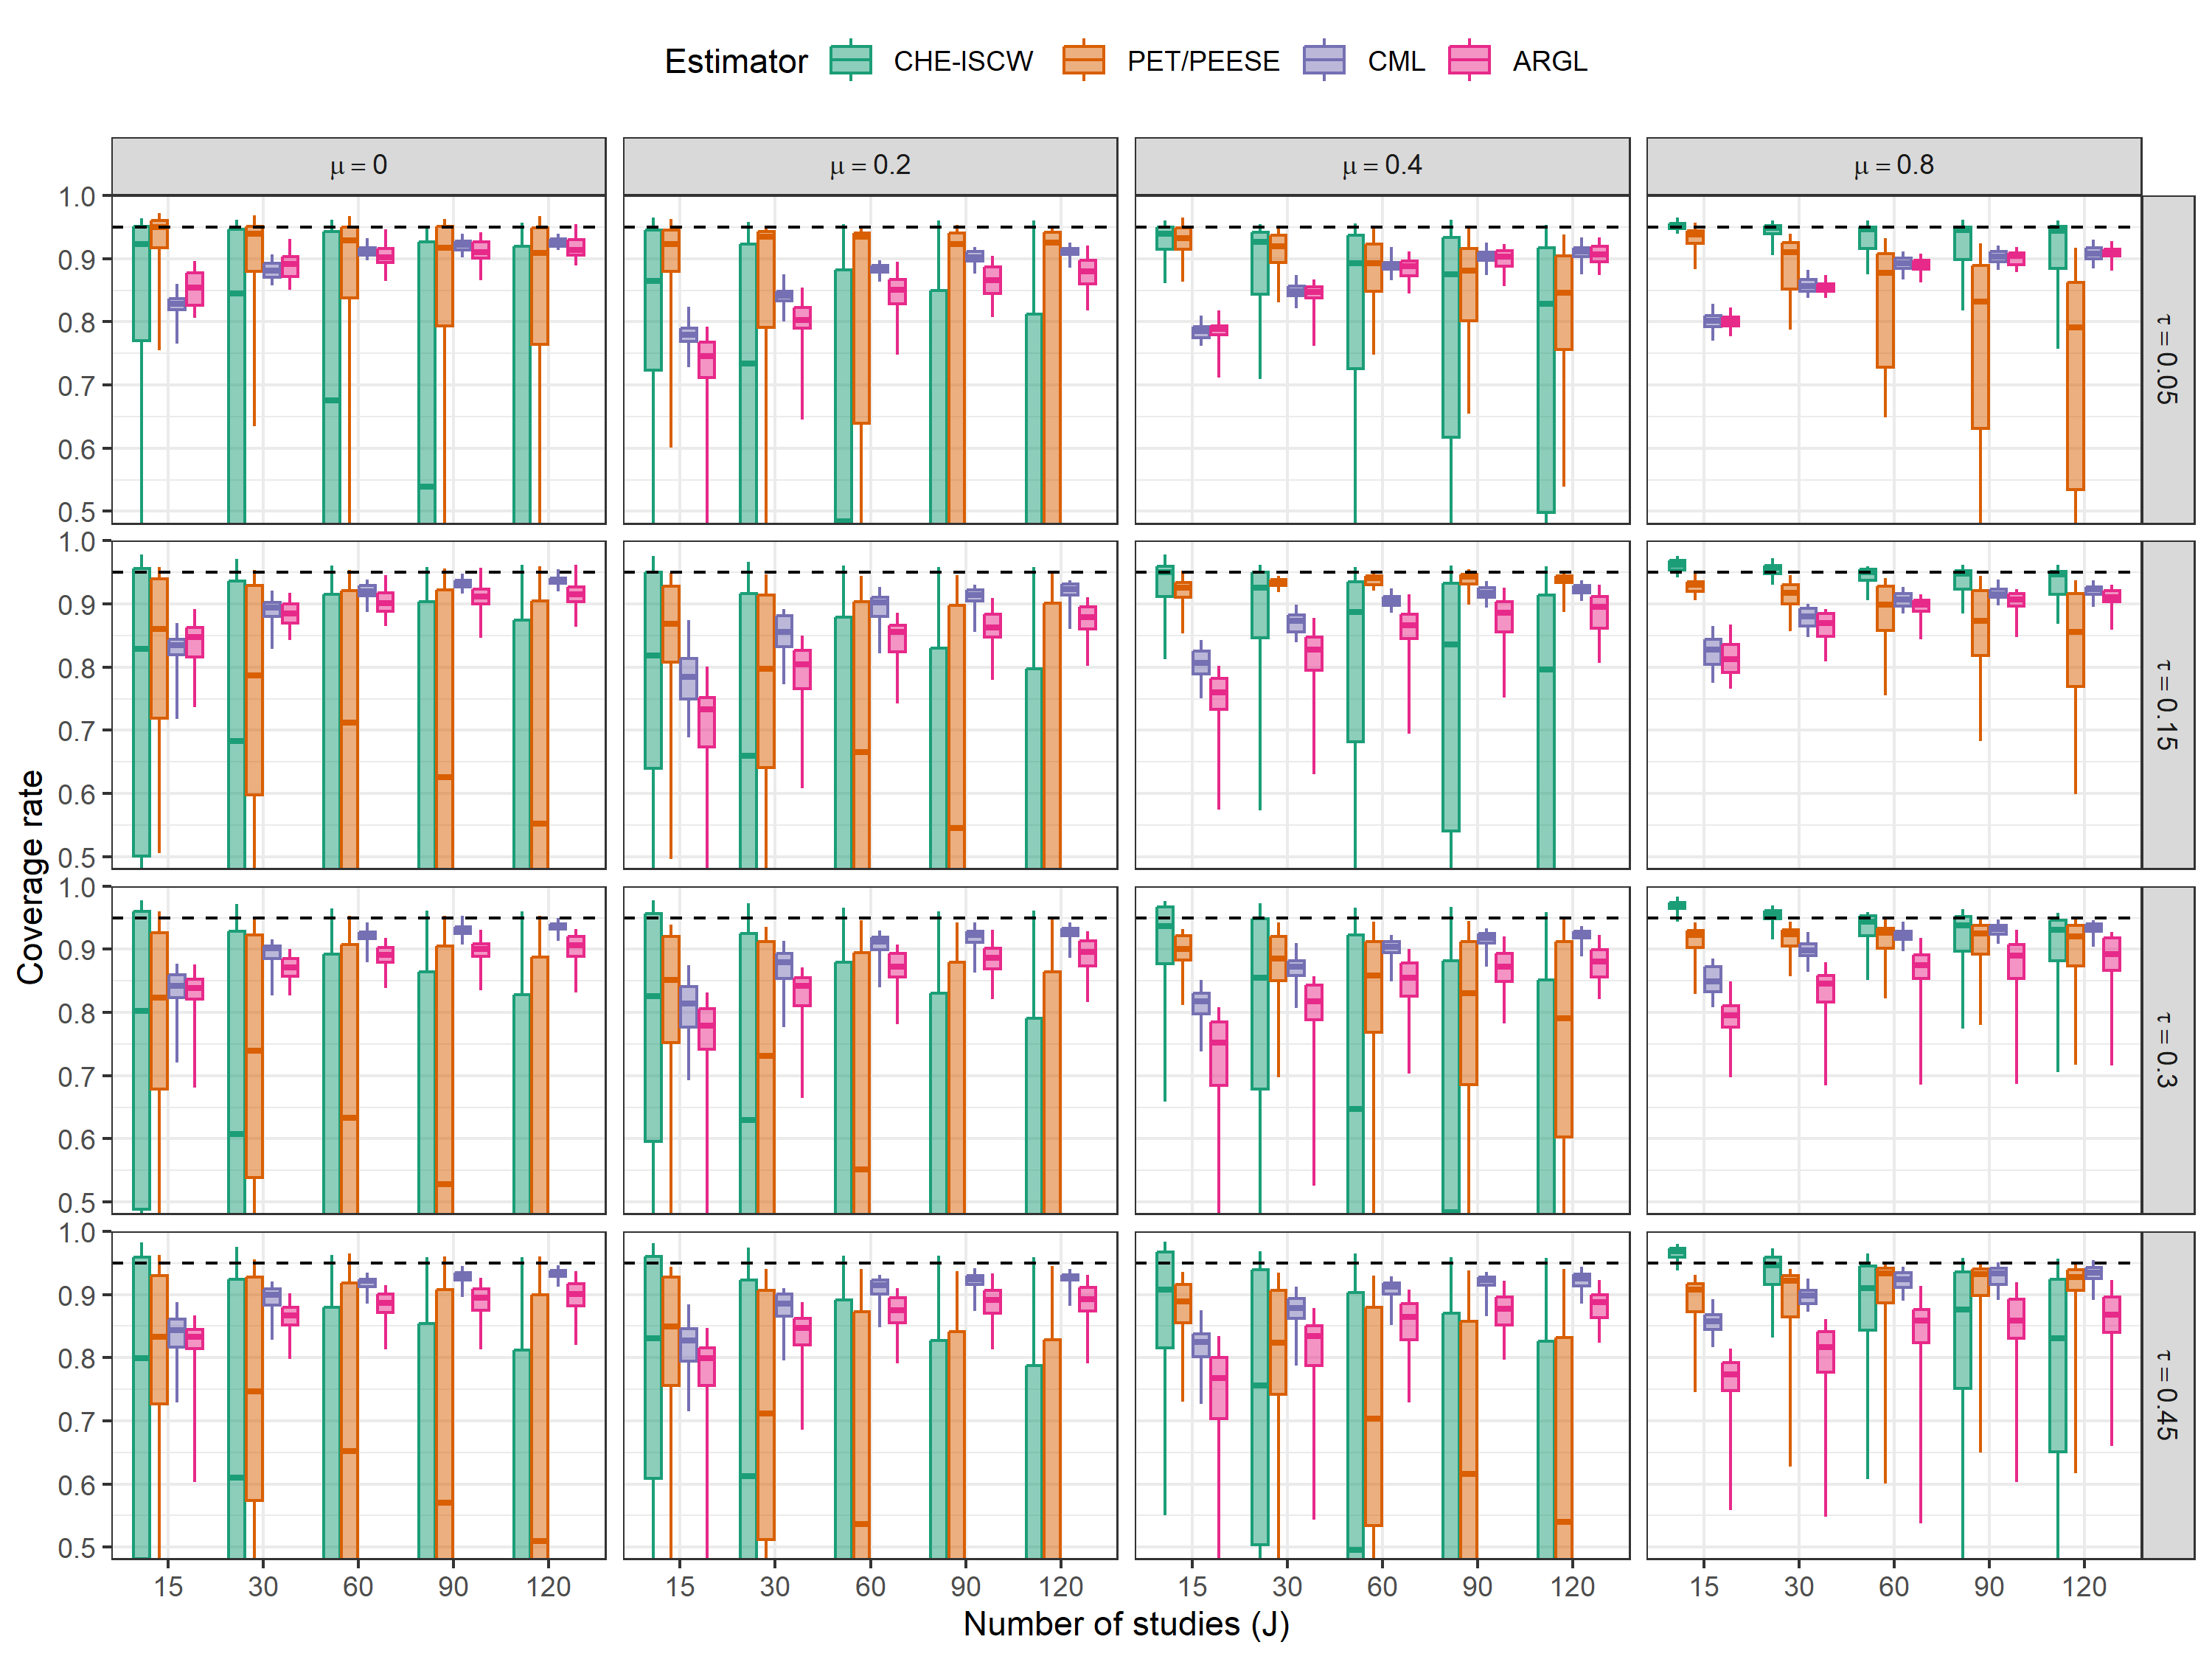
\includegraphics{selection_models_draft_files/figure-latex/comparison-coverage-1} \caption{Coverage levels of confidence intervals based for average effect size based on cluster-robust variance approximations, by number of studies, average SMD, and between-study heterogeneity. Dashed lines correspond to the nominal confidence level of 0.95. Coverage rates of the CHE-ISCW and PET/PEESE intervals are not depicted when they fall below 0.5}\label{fig:comparison-coverage}
\end{sidewaysfigure}

Bootstrap intervals for the step-function model provide more accurate coverage levels.
Due to the computational demands of bootstrapping, we evaluated the bootstrap confidence intervals under a more limited range of data-generating conditions, including a maximum sample size of \(J = 60\). Figure \ref{fig:CML-coverage} depicts the coverage levels of confidence intervals based on the CML estimator, including intervals based on large-sample cluster-robust variance methods and percentile intervals using either multinomial (non-parametric) or exponential (fractional reweighted) bootstrap resampling.
Although none of the intervals provide exactly nominal coverage, both versions of the percentile bootstrap intervals have coverage that is closer to nominal than the intervals based on cluster-robust variance estimation.
In particular, the percentile intervals with multinomial bootstrap re-sampling provided the best coverage levels, exceeding 90\% coverage across data-generating conditions when the number of studies was 30 or greater.
Coverage levels of the other bootstrap intervals, including studentized, basic, and BCa intervals, were not as accurate as percentile intervals (see Supplementary Figure \ref{fig:CML-coverage-full} for detailed results).
Coverage levels of intervals based on the ARGL estimator followed very similar patterns to those for the CML estimator (Supplementary Figure \ref{fig:ARGL-coverage-full}).

\begin{sidewaysfigure}
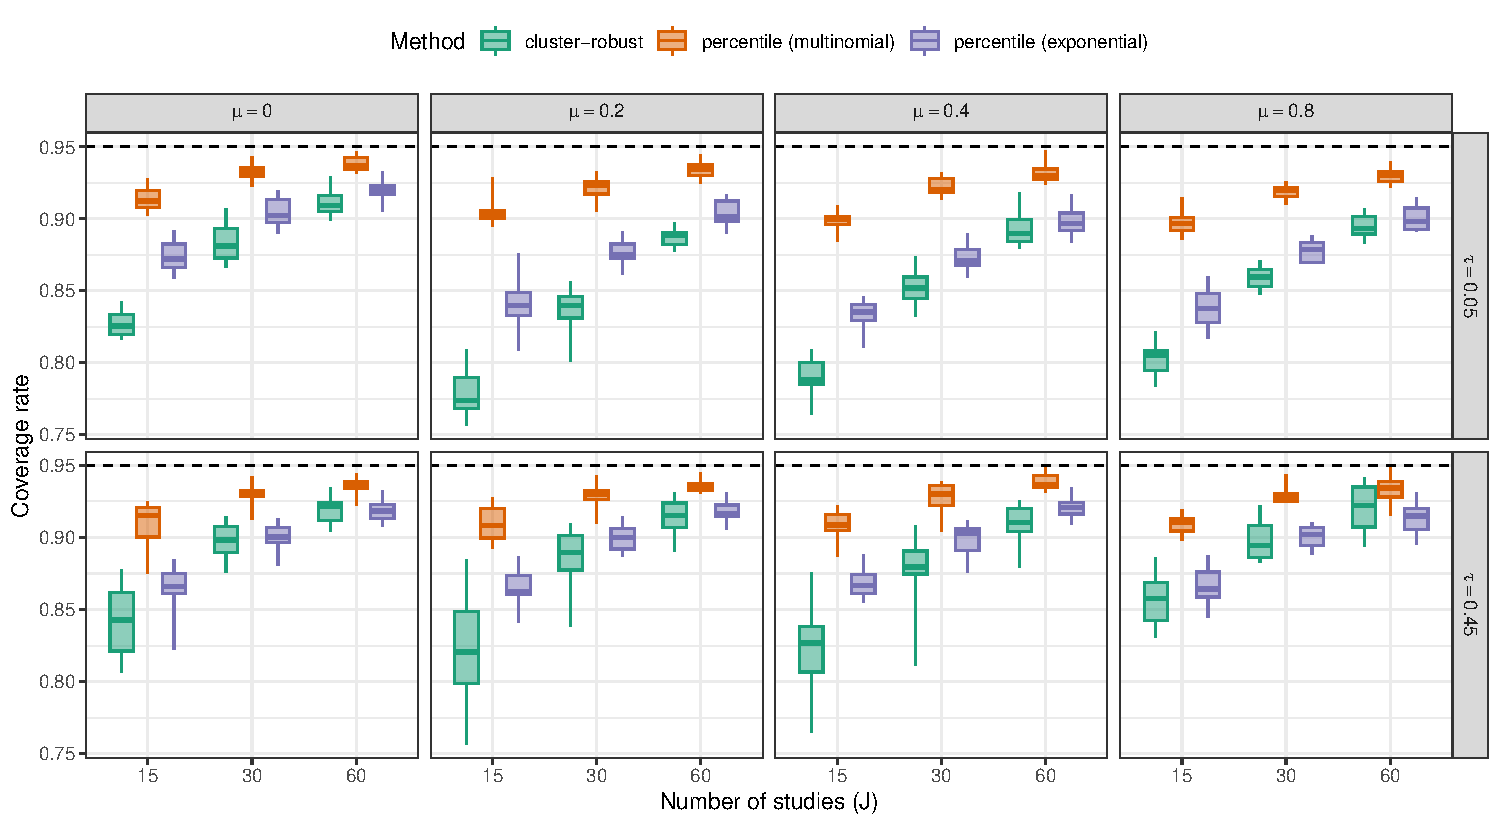
\includegraphics{selection_models_draft_files/figure-latex/CML-coverage-1} \caption{Coverage levels of confidence intervals based on the CML estimator of average effect size by number of studies, average SMD, and between-study heterogeneity. Dashed lines correspond to the nominal confidence level of 0.95.}\label{fig:CML-coverage}
\end{sidewaysfigure}

\subsection{Effect Size Variance}\label{effect-size-variance}

We briefly consider estimation of the marginal heterogeneity of the effect size distribution, for which the CHE, CML, and ARGL methods are all relevant.\footnote{We omitted the variance estimator from the CHE-ISCW method because it is identical to that of CHE.}
Figure \ref{fig:heterogeneity-bias} depicts the bias for the CHE, CML, and ARGL estimators of log-heterogeneity \(\gamma = \log(\tau^2)\).
In most conditions, the estimators are biased in the negative direction. Bias is high for all three estimators in conditions where the between-study heterogeneity is low (\(\tau = 0.05\)) with bias improving as between-study heterogeneity increases. The CML estimator is less strongly biased than the CHE estimator under conditions where there is strong selection.
However, the ARGL estimator is badly biased downward, especially under conditions where selection is strong, average SMD is low and between-study heterogeneity is low.
Figure \ref{fig:heterogeneity-rmse} depicts the scaled RMSE for estimators of log-heterogeneity, with Figures \ref{fig:heterogeneity-rmse-ARGL-CHE} and \ref{fig:heterogeneity-rmse-ARGL-CML} providing greater detail about the relative accuracy of the three methods.
Under nearly all conditions, the CML estimator is much more accurate than the ARGL estimator.
The RMSE of CML is smaller than that of CHE under some but not all conditions; the former performs better under conditions where selection is strong, average SMD is low, between-study heterogeneity is large, and sample size is large.
However, just as with the estimators of average effect size, the CHE estimator is more accurate when selection is mild or absent, leading to a bias-variance trade-off.

\subsection{Selection Parameter}\label{selection-parameter}

The CML and ARGL methods both estimate the log-selection parameter of the step-function model, a parameter that may be of substantive interest.
Figure \ref{fig:selection-bias} shows that the bias of the two estimators is similar: Both show bias close to zero under conditions with low average SMD and high between-study heterogeneity but have large negative biases under conditions with strong selection probability and high average SMD, especially with low between-study heterogeneity.
Figure \ref{fig:selection-rmse} depicts the RMSE for the ARGL and CML estimators of the log-selection parameter with Figure \ref{fig:selection-rmse-ARGL-CML} providing a more detailed view of the relative accuracy of the ARGL versus the CML estimators.
The CML estimator of the selection parameter generally outperforms the ARGL estimator, especially under conditions with strong selection.
Figures \ref{fig:CML-zeta-coverage-full} and \ref{fig:ARGL-zeta-coverage-full} depict the confidence interval coverage of the two estimators with various combinations of cluster bootstrapping methods and bootstrap confidence interval estimation approaches.
Broadly, none of the methods provide coverage rates that are close to the nominal 95\% level.

\section{Discussion}\label{discussion}

We have described and evaluated several methods for estimating Vevea and Hedges (1995) step-function selection models while accounting for dependent effect sizes, a common feature of meta-analyses in social science fields.
We focused on the step-function selection model because it offers a number of advantages over other available methods for diagnosing and correcting selective reporting bias.
First, step-function models are generative, in that they include parameters describing the selective reporting process under simple yet plausible forms of selective reporting connected to statistical significance.
In contrast, regression-based estimators such as PET/PEESE (Stanley \& Doucouliagos, 2014) or the endogenous kink meta-regression (Bom \& Rachinger, 2019) are agnostic as to selection mechanisms and thus are only indirectly informative about the strength or form of selection.
The Vevea and Hedges (1995) step-function model also embeds a familiar evidence-generating model that allows for heterogeneity of effects through inclusion of random effects and predictors of average effect size (i.e., meta-regression).
In contrast, well-known methods such as trim-and-fill (Duval \& Tweedie, 2000a, 2000b) and recent proposals such as \(p\)-curve (Simonsohn et al., 2014) and \(p\)-uniform (Aert et al., 2016; Assen et al., 2015) are not as flexible and have been found to perform poorly when effects are heterogeneous (Carter et al., 2019).

We treated the step-function model as a description of the \emph{marginal} distribution of the effect size estimates, effectively ignoring the dependence structure for purposes of estimating the model but accounting for it using cluster-robust sandwich estimation or clustered bootstrap inference.
This strategy is appealing for its feasibility and because it connects to a selection process in which each individual effect size is selected on the basis of its statistical significance.
We also implemented and studied two estimation methods for the marginal step-function model, composite marginal likelihood estimation and augmented-and-reweighted Gaussian likelihood estimation, and two inference strategies, based on either cluster-robust sandwich estimators or clustered bootstrap resampling methods.

Our simulations examined how well these estimators and inference techniques perform for recovering the average effect size under a selection process with a single step (at \(\alpha_1 = .025\)), relative to estimators that account for dependence but not selection (i.e., the CHE-ISCW model) and to a variant of PET/PEESE that uses RVE.
Across an extensive range of conditions, we found that both estimators of the marginal step-function model showed little bias, which was consistently smaller than the bias of PET/PEESE and much smaller than the bias of CHE-ISCW under conditions with meaningful selective reporting.
However, the selection model estimators face a bias-variance trade-off.
The bias reduction from using the selection model comes at the cost of increased variance from using a marginal model. As a result, the step-function estimators are less accurate than the CHE-ISCW estimator under conditions where selective reporting is not strong or does not create meaningful bias.
The marginal step-function model estimators also have better coverage compared to the other methods, with coverage rates of the cluster-bootstrapped confidence intervals approaching the nominal level of 0.95 for larger sample sizes.
Compared to the ARGL estimator, the CML estimator of the marginal mean was usually more accurate and had confidence interval coverage rates closer to nominal levels, although differences are fairly small.
CML consistently out-performed ARGL for estimating between-study heterogeneity and the strength of selective reporting.

\subsection{Limitations and Further Directions}\label{limitations-and-further-directions}

Both the methods we have developed and the findings from our simulation study have limitations that are important to recognize.
On a conceptual level, the strategy of modeling the marginal distribution of effect sizes presents several limitations.
First, such models do not attempt to describe the structure of dependence among effect size estimates drawn from the same sample, but instead describe only the overall average and overall degree of heterogeneity of the effect size distribution.
Because of this, they do not fully align with contemporary approaches to summary meta-analysis and meta-regression analysis, which emphasize use of models that align with the hierarchical structure of dependent effect sizes (Pustejovsky \& Tipton, 2022; Van den Noortgate et al., 2013).

Second, focusing on the marginal distribution likely entails some loss of precision in parameter estimates.
Accounting for the dependence structure would allow for construction of more efficient estimators of the parameters of the evidence-generating process.
A useful direction for further research would be to explore how to refine the CML and ARGL estimators by incorporating analytic weights connected with the dependence structure of the effect sizes.

Third, the marginal model provides no way to distinguish between study-level publication bias and effect-level selective outcome reporting.
This strategy therefore precludes examination of more nuanced forms of selection, such as one where the probability that a given effect size is reported depends on the significance levels of other effect size estimates drawn from the same sample or on some broader feature of the study's results.
This strikes us as an area in need of further theoretical development---even simply to catalog a wider variety of plausible selective reporting mechanisms.
However, developing more nuanced models would require shifting to estimation frameworks that can handle multivariate models, such as multivariate likelihood-based estimation or pairwise composite likelihood methods (e.g., Rao et al., 2013; Yi et al., 2016).

In addition to conceptual limitations, our simulation findings also need to be interpreted cautiously in light of the study's scope limitations.
First, although we tried to cover a wide range of plausible conditions in the simulation study (3,840 conditions for the full simulation and 288 conditions for the bootstrap simulation), the results are only generalizable to the data-generating process presented in the study.
Of particular note, the evidence-generating process we used followed a CHE effects model with primary study sample sizes and the number of effect sizes per study drawn from an empirical distribution of educational research studies.
The performance of the step-function selection models and alternative selective reporting adjustments could vary depending on features of studies included in the synthesis, such as studies drawn from areas of research that tend to use very small or very large samples or that tend to assess a larger number of outcomes.
Likewise, there remains a need to investigate the robustness of the models to other evidence-generating processes, such as non-normal random effects distributions (Hedges \& Vevea, 1996).

Second, the simulations examined the step-function selection model using a selection process that was compatible with the assumed model, in which the probability that an effect size was reported followed a step function in the one-sided \emph{p}-value with a threshold at \(\alpha_1 = .025\).
Chen and Pustejovsky (2024) examined the performance of one-step and two-step selection model estimators under conditions when the true data-generating process involved a two-step selection process with an additional threshold at \(\alpha_2 = .500\).
Their results indicated that a one-step model could be more accurate (i.e., lower RMSE) than a more complex two-step model---even if the former is mis-specified.
It may require a relatively large number of primary studies to feasibly estimate models that include multiple steps in the selection function.
Nonetheless, there may be meta-analytic datasets where a more complex set of steps is more appropriate, such as when the data include a substantial number of negative effect size estimates.

Third and related to the previous point, the simulations were limited to evidence-generating processes that did not involve systematic predictors of the effect size distribution and where the strength of selective reporting was uniform and solely dependent on the p-value of each individual effect size.
There may be other factors besides statistical significance of findings that affect a study's publication status.
For instance, results from pre-registered replication studies might be insulated from selective reporting or subject to different reporting pressures than other forms of primary research (Van Aert, 2025).
Further evaluation of the CML and ARGL estimators is warranted to assess their performance in models involving moderators and their robustness to other selection mechanisms.
In further development of step-function selection models, it may prove useful to model variation in the strength of reporting as a function of study characteristics such as pre-registration status (Coburn \& Vevea, 2015).

Fourth and finally, the simulation findings we have reported here focused mostly on the performance of the estimators and confidence intervals for the overall average effect size.
We have not directly evaluated how well the estimators work as diagnostic \emph{tests} for the presence of selective reporting of study results, although the below-nominal coverage rates of confidence intervals for the selection parameter suggests that they may not work well diagnostically.
In univariate random effects models, likelihood ratio tests based on step-function selection models have been found to provide much stronger power for detecting selective reporting compared to alternatives such as Egger's regression or non-parametric symmetry tests (Pustejovsky \& Rodgers, 2019).
Extension of such tests for meta-analyses of dependent effect sizes requires further development.

\subsection{Implications for Practice}\label{implications-for-practice}

The potential for selective reporting of primary study results to distort and create biases in meta-analytic results is simultaneously of great concern to meta-analysts and a vexing problem to address---even in the simpler context of meta-analysis of independent effects (i.e., when each sample reports at most a single effect size estimate).
The challenge of detecting and adjusting for bias from selective reporting is all the more challenging in a corpus of primary study results that includes dependent effect sizes.
Nonetheless, meta-analysts must critically evaluate the evidence summarized in a synthesis, and this includes weighing the potential for bias from selective reporting and selective publication.

Considering both the simulation results and the limitations that we have described, we

\begin{itemize}
\tightlist
\item
  Current practice is spaghetti-against-the-wall.

  \begin{itemize}
  \tightlist
  \item
    Past methodological work indicates that the performance of most available bias-correction methods is variable
  \item
    Carter et al., McShane et al.~argue that there needs to be more discerning use of bias-correction methods, with attention to the conditions under which a given method provides credible adjusted estimates.
  \end{itemize}
\end{itemize}

\section*{Author Contributions}\label{author-contributions}
\addcontentsline{toc}{section}{Author Contributions}

\textbf{JEP:} Conceptualization, Methodology, Software, Validation, Formal Analysis, Investigation, Resources, Writing - original draft, Writing - review \& editing, Supervision \textbf{MJ:} Methodology, Software, Validation, Formal Analysis, Investigation, Writing - original draft, Writing - review \& editing, Visualization \textbf{MC:} Conceptualization, Methodology, Investigation, Writing - original draft, Writing - review \& editing, Project administration, Funding acquisition

\newpage

\section*{References}\label{references}
\addcontentsline{toc}{section}{References}

\begingroup
\setlength{\parindent}{-0.5in}

\phantomsection\label{refs}
\begin{CSLReferences}{1}{0}
\bibitem[\citeproctext]{ref-vanaert2016conducting}
Aert, R. C. M. van, Wicherts, J. M., \& Assen, M. A. L. M. van. (2016). Conducting meta-analyses based on \emph{p} values: Reservations and recommendations for applying \emph{p} -uniform and \emph{p} -curve. \emph{Perspectives on Psychological Science}, \emph{11}(5), 713--729. \url{https://doi.org/10.1177/1745691616650874}

\bibitem[\citeproctext]{ref-VanAssen2015meta}
Assen, M. A. L. M. van, Van Aert, R. C. M., \& Wicherts, J. M. (2015). {Meta-analysis using effect size distributions of only statistically significant studies}. \emph{Psychological Methods}, \emph{20}(3), 293--309. https://doi.org/\url{http://dx.doi.org/10.1037/met0000025}

\bibitem[\citeproctext]{ref-begg1994operating}
Begg, C. B., \& Mazumdar, M. (1994). Operating characteristics of a rank correlation test for publication bias. \emph{Biometrics}, 1088--1101.

\bibitem[\citeproctext]{ref-bom2019kinked}
Bom, P. R. D., \& Rachinger, H. (2019). A kinked meta-regression model for publication bias correction. \emph{Research Synthesis Methods}, \emph{10}(4), 497--514. \url{https://doi.org/10.1002/jrsm.1352}

\bibitem[\citeproctext]{ref-boos2000montecarlo}
Boos, D. D., \& Zhang, J. (2000). Monte carlo evaluation of resampling-based hypothesis tests. \emph{Journal of the American Statistical Association}, \emph{95}(450), 486--492. \url{https://doi.org/10.1080/01621459.2000.10474226}

\bibitem[\citeproctext]{ref-borenstein2019effect}
Borenstein, M., \& Hedges, L. V. (2019). Effect sizes for meta-analysis. \emph{The Handbook of Research Synthesis and Meta-Analysis}, \emph{3}, 207--243.

\bibitem[\citeproctext]{ref-carter2015series}
Carter, E. C., Kofler, L. M., Forster, D. E., \& McCullough, M. E. (2015). A series of meta-analytic tests of the depletion effect: Self-control does not seem to rely on a limited resource. \emph{Journal of Experimental Psychology: General}, \emph{144}(4), 796.

\bibitem[\citeproctext]{ref-carter2019correcting}
Carter, E. C., Schönbrodt, F. D., Gervais, W. M., \& Hilgard, J. (2019). Correcting for bias in psychology: A comparison of meta-analytic methods. \emph{Advances in Methods and Practices in Psychological Science}, \emph{2}(2), 115--144.

\bibitem[\citeproctext]{ref-CHTC}
Center for High Throughput Computing. (2006). \emph{Center for high throughput computing}. Center for High Throughput Computing. \url{https://doi.org/10.21231/GNT1-HW21}

\bibitem[\citeproctext]{ref-chan2004empirical}
Chan, A.-W., Hróbjartsson, A., Haahr, M. T., Gøtzsche, P. C., \& Altman, D. G. (2004). Empirical evidence for selective reporting of outcomes in randomized trials: Comparison of protocols to published articles. \emph{Jama}, \emph{291}(20), 2457--2465.

\bibitem[\citeproctext]{ref-chen2024adapting}
Chen, M., \& Pustejovsky, J. E. (2024). \emph{Adapting methods for correcting selective reporting bias in meta-analysis of dependent effect sizes}. \url{https://doi.org/10.31222/osf.io/jq52s}

\bibitem[\citeproctext]{ref-citkowicz2017parsimonious}
Citkowicz, M., \& Vevea, J. L. (2017). {A parsimonious weight function for modeling publication bias}. \emph{Psychological Methods}, \emph{22}(1), 28--41. \url{https://doi.org/10.1037/met0000119}

\bibitem[\citeproctext]{ref-Coburn2015publication}
Coburn, K. M., \& Vevea, J. L. (2015). {Publication bias as a function of study characteristics}. \emph{Psychological Methods}, \emph{20}(3), 310--330. \url{https://doi.org/10.1037/met0000046}

\bibitem[\citeproctext]{ref-copas1999what}
Copas, J. B. (1999). What works?: {Selectivity} models and meta-analysis. \emph{Journal of the Royal Statistical Society Series A: Statistics in Society}, \emph{162}(1), 95--109. \url{https://doi.org/10.1111/1467-985X.00123}

\bibitem[\citeproctext]{ref-copas1997inference}
Copas, J. B., \& Li, H. G. (1997). Inference for non-random samples. \emph{Journal of the Royal Statistical Society Series B: Statistical Methodology}, \emph{59}(1), 55--95. \url{https://doi.org/10.1111/1467-9868.00055}

\bibitem[\citeproctext]{ref-Copas2001sensitivity}
Copas, J. B., \& Shi, J. Q. (2001). {A sensitivity analysis for publication bias in systematic reviews.} \emph{Statistical Methods in Medical Research}, \emph{10}, 251--265.

\bibitem[\citeproctext]{ref-cox2004note}
Cox, D. R., \& Reid, N. (2004). A note on pseudolikelihood constructed from marginal densities. \emph{Biometrika}, \emph{91}(3), 729--737. \url{https://doi.org/10.1093/biomet/91.3.729}

\bibitem[\citeproctext]{ref-davison1997bootstrap}
Davison, A. C., \& Hinkley, D. V. (1997). \emph{Bootstrap methods and their applications}. Cambridge University Press.

\bibitem[\citeproctext]{ref-dear1992approach}
Dear, K. B. G., \& Begg, C. B. (1992). {An approach for assessing publication bias prior to performing a meta-analysis}. \emph{Statistical Science}, \emph{7}(2), 237--245.

\bibitem[\citeproctext]{ref-duval2000nonparametric}
Duval, S., \& Tweedie, R. (2000a). A nonparametric {``trim and fill''} method of accounting for publication bias in meta-analysis. \emph{Journal of the American Statistical Association}, \emph{95}(449), 89--98.

\bibitem[\citeproctext]{ref-duval2000trim}
Duval, S., \& Tweedie, R. (2000b). Trim and fill: A simple funnel-plot--based method of testing and adjusting for publication bias in meta-analysis. \emph{Biometrics}, \emph{56}(2), 455--463.

\bibitem[\citeproctext]{ref-efron1987better}
Efron, B. (1987). Better bootstrap confidence intervals. \emph{Journal of the American Statistical Association}, \emph{82}(397), 171--185. \url{https://doi.org/10.1080/01621459.1987.10478410}

\bibitem[\citeproctext]{ref-egger1997bias}
Egger, M., Smith, G. D., Schneider, M., \& Minder, C. (1997). Bias in meta-analysis detected by a simple, graphical test. \emph{BMJ}, \emph{315}(7109), 629--634.

\bibitem[\citeproctext]{ref-fernandezcastilla2019detecting}
Fernández-Castilla, B., Declercq, L., Jamshidi, L., Beretvas, S. N., Onghena, P., \& Van den Noortgate, W. (2019). Detecting selection bias in meta-analyses with multiple outcomes: A simulation study. \emph{The Journal of Experimental Education}, 1--20. \url{https://doi.org/10.1080/00220973.2019.1582470}

\bibitem[\citeproctext]{ref-franco2016underreporting}
Franco, A., Malhotra, N., \& Simonovits, G. (2016). Underreporting in psychology experiments: Evidence from a study registry. \emph{Social Psychological and Personality Science}, \emph{7}(1), 8--12. \url{https://doi.org/10.1177/1948550615598377}

\bibitem[\citeproctext]{ref-greenwald1975prejudice}
Greenwald, A. G. (1975). Consequences of prejudice against the null hypothesis. \emph{Psychological Bulletin}, \emph{82}(1), 1--20. \url{https://doi.org/10.1037/h0076157}

\bibitem[\citeproctext]{ref-hagger2010ego}
Hagger, M. S., Wood, C., Stiff, C., \& Chatzisarantis, N. L. D. (2010). Ego depletion and the strength model of self-control: {A} meta-analysis. \emph{Psychological Bulletin}, \emph{136}(4), 495--525. \url{https://doi.org/10.1037/a0019486}

\bibitem[\citeproctext]{ref-harbord2006modified}
Harbord, R. M., Egger, M., \& Sterne, J. A. (2006). A modified test for small-study effects in meta-analyses of controlled trials with binary endpoints. \emph{Statistics in Medicine}, \emph{25}(20), 3443--3457.

\bibitem[\citeproctext]{ref-nleqslv}
Hasselman, B. (2023). \emph{Nleqslv: Solve systems of nonlinear equations}. \url{https://CRAN.R-project.org/package=nleqslv}

\bibitem[\citeproctext]{ref-hedges1984estimation}
Hedges, L. V. (1984). Estimation of effect size under nonrandom sampling: The effects of censoring studies yielding statistically insignificant mean differences. \emph{Journal of Educational Statistics}, \emph{9}(1), 61--85.

\bibitem[\citeproctext]{ref-hedges1992modeling}
Hedges, L. V. (1992). Modeling publication selection effects in meta-analysis. \emph{Statistical Science}, \emph{7}(2), 246--255.

\bibitem[\citeproctext]{ref-Hedges2010robust}
Hedges, L. V., Tipton, E., \& Johnson, M. C. (2010). {Robust variance estimation in meta-regression with dependent effect size estimates}. \emph{Research Synthesis Methods}, \emph{1}(1), 39--65. \url{https://doi.org/10.1002/jrsm.5}

\bibitem[\citeproctext]{ref-hedges2005selection}
Hedges, L. V., \& Vevea, J. (2005). Selection method approaches. In H. R. Rothstein, A. J. Sutton, \& M. Borenstein (Eds.), \emph{Publication bias in meta-analysis} (pp. 145--174). {John Wiley \& Sons, Ltd}. \url{https://doi.org/10.1002/0470870168.ch9}

\bibitem[\citeproctext]{ref-Hedges1996estimating}
Hedges, L. V., \& Vevea, J. L. (1996). {Estimating effect size under publication bias: Small sample properties and robustness of a random effects selection model}. \emph{Journal of Educational and Behavioral Statistics}, \emph{21}(4), 299. \url{https://doi.org/10.3102/10769986021004299}

\bibitem[\citeproctext]{ref-iyengar1988selection}
Iyengar, S., \& Greenhouse, J. B. (1988). Selection {Models} and the {File} {Drawer} {Problem}. \emph{Statistical Science}, \emph{3}(1), 109--117. \url{https://doi.org/10.1214/ss/1177013012}

\bibitem[\citeproctext]{ref-john2012measuring}
John, L. K., Loewenstein, G., \& Prelec, D. (2012). Measuring the prevalence of questionable research practices with incentives for truth telling. \emph{Psychological Science}, \emph{23}(5), 524--532.

\bibitem[\citeproctext]{ref-simhelpers}
Joshi, M., \& Pustejovsky, J. E. (2024). \emph{Simhelpers: Helper functions for simulation studies}. \url{https://meghapsimatrix.github.io/simhelpers/}

\bibitem[\citeproctext]{ref-joshi2022cluster}
Joshi, M., Pustejovsky, J. E., \& Beretvas, S. N. (2022). Cluster Wild Bootstrapping to Handle Dependent Effect Sizes in Meta-Analysis with a Small Number of Studies. \emph{Research Synthesis Methods}, \emph{13}(4), 457--477. \url{https://doi.org/10.1002/jrsm.1554}

\bibitem[\citeproctext]{ref-konstantopoulos2011fixed}
Konstantopoulos, S. (2011). Fixed effects and variance components estimation in three-level meta-analysis: {Three}-level meta-analysis. \emph{Research Synthesis Methods}, \emph{2}(1), 61--76. \url{https://doi.org/10.1002/jrsm.35}

\bibitem[\citeproctext]{ref-kossmeier2020PowerEnhanced}
Kossmeier, M., Tran, U. S., \& Voracek, M. (2020). Power-enhanced funnel plots for meta-analysis. \emph{Zeitschrift Für Psychologie}. \url{https://econtent.hogrefe.com/doi/10.1027/2151-2604/a000392}

\bibitem[\citeproctext]{ref-kraft2020interpreting}
Kraft, M. A. (2020). Interpreting effect sizes of education interventions. \emph{Educational Researcher}, \emph{49}(4), 241--253.

\bibitem[\citeproctext]{ref-lancee2017outcome}
Lancee, M., Lemmens, C., Kahn, R., Vinkers, C., \& Luykx, J. (2017). Outcome reporting bias in randomized-controlled trials investigating antipsychotic drugs. \emph{Translational Psychiatry}, \emph{7}(9), e1232--e1232.

\bibitem[\citeproctext]{ref-light1984Summing}
Light, R. J., \& Pillemer, D. B. (1984). \emph{Summing {Up}}. {Harvard University Press}. \url{https://books.google.com?id=qel3lAm4K6gC}

\bibitem[\citeproctext]{ref-lindsay1988composite}
Lindsay, B. G. (1988). Composite likelihood methods. In N. U. Prabhu (Ed.), \emph{Contemporary {Mathematics}} (Vol. 80, pp. 221--239). American Mathematical Society. \url{https://doi.org/10.1090/conm/080/999014}

\bibitem[\citeproctext]{ref-macaskill2001comparison}
Macaskill, P., Walter, S. D., \& Irwig, L. (2001). A comparison of methods to detect publication bias in meta-analysis. \emph{Statistics in Medicine}, \emph{20}(4), 641--654. \url{https://doi.org/10.1002/sim.698}

\bibitem[\citeproctext]{ref-marksanglin2020historical}
Marks‐Anglin, A., \& Chen, Y. (2020). A historical review of publication bias. \emph{Research Synthesis Methods}, \emph{11}(6), 725--742. \url{https://doi.org/10.1002/jrsm.1452}

\bibitem[\citeproctext]{ref-mathur2020sensitivity}
Mathur, M. B., \& VanderWeele, T. J. (2020). Sensitivity analysis for publication bias in meta‐analyses. \emph{Journal of the Royal Statistical Society: Series C (Applied Statistics)}, \emph{69}(5), 1091--1119. \url{https://doi.org/10.1111/rssc.12440}

\bibitem[\citeproctext]{ref-moreno2012generalized}
Moreno, S. G., Sutton, A. J., Thompson, J. R., Ades, A., Abrams, K. R., \& Cooper, N. J. (2012). A generalized weighting regression-derived meta-analysis estimator robust to small-study effects and heterogeneity. \emph{Statistics in Medicine}, \emph{31}(14), 1407--1417.

\bibitem[\citeproctext]{ref-nakagawa2023quantitative}
Nakagawa, S., Yang, Y., Macartney, E. L., Spake, R., \& Lagisz, M. (2023). Quantitative evidence synthesis: A practical guide on meta-analysis, meta-regression, and publication bias tests for environmental sciences. \emph{Environmental Evidence}, \emph{12}(1), 8. \url{https://doi.org/10.1186/s13750-023-00301-6}

\bibitem[\citeproctext]{ref-optimx}
Nash, J. C., \& Varadhan, R. (2011). Unifying optimization algorithms to aid software system users: {optimx} for {R}. \emph{Journal of Statistical Software}, \emph{43}(9), 1--14. \url{https://doi.org/10.18637/jss.v043.i09}

\bibitem[\citeproctext]{ref-Nelson1986significance}
Nelson, N., Rosenthal, R., \& Rosnow, R. L. (1986). Interpretation of significance levels and effect sizes by psychological researchers. \emph{American Psychologist}, \emph{41}(11), 1299--1301. \url{https://doi.org/10.1037/0003-066X.41.11.1299}

\bibitem[\citeproctext]{ref-oBoyle2017chrysalis}
O'Boyle Jr, E. H., Banks, G. C., \& Gonzalez-Mulé, E. (2017). The chrysalis effect: How ugly initial results metamorphosize into beautiful articles. \emph{Journal of Management}, \emph{43}(2), 376--399.

\bibitem[\citeproctext]{ref-peters2006comparison}
Peters, J. L., Sutton, A. J., Jones, D. R., Abrams, K. R., \& Rushton, L. (2006). Comparison of two methods to detect publication bias in meta-analysis. \emph{Journal of the American Medical Association}, \emph{295}(6), 676--680.

\bibitem[\citeproctext]{ref-pigott2013outcome}
Pigott, T. D., Valentine, J. C., Polanin, J. R., Williams, R. T., \& Canada, D. D. (2013). Outcome-reporting bias in education research. \emph{Educational Researcher}, \emph{42}(8), 424--432.

\bibitem[\citeproctext]{ref-preston2004adjusting}
Preston, C., Ashby, D., \& Smyth, R. (2004). Adjusting for publication bias: Modelling the selection process. \emph{Journal of Evaluation in Clinical Practice}, \emph{10}(2), 313--322. \url{https://doi.org/10.1111/j.1365-2753.2003.00457.x}

\bibitem[\citeproctext]{ref-clubSandwich}
Pustejovsky, J. E. (2024). \emph{clubSandwich: Cluster-robust (sandwich) variance estimators with small-sample corrections}. \url{https://CRAN.R-project.org/package=clubSandwich}

\bibitem[\citeproctext]{ref-metaselection}
Pustejovsky, J. E., \& Joshi, M. (2025). \emph{Metaselection: Meta-analytic selection models with cluster-robust and cluster-bootstrap standard errors for dependent effect size estimates}. \url{https://github.com/jepusto/metaselection}

\bibitem[\citeproctext]{ref-pustejovsky2019testing}
Pustejovsky, J. E., \& Rodgers, M. A. (2019). Testing for funnel plot asymmetry of standardized mean differences. \emph{Research Synthesis Methods}, \emph{10}(1), 57--71.

\bibitem[\citeproctext]{ref-pustejovsky2022preventionscience}
Pustejovsky, J. E., \& Tipton, E. (2022). Meta-Analysis with Robust Variance Estimation: {Expanding} the Range of Working Models. \emph{Prevention Science}, \emph{23}, 425--438. \url{https://doi.org/10.1016/j.jsp.2018.02.003}

\bibitem[\citeproctext]{ref-rcoreteam}
R Core Team. (2025). \emph{R: A language and environment for statistical computing}. R Foundation for Statistical Computing. \url{https://www.R-project.org/}

\bibitem[\citeproctext]{ref-rao2013weighted}
Rao, J. N. K., Verret, F., \& Hidiroglou, M. A. (2013). A weighted composite likelihood approach to inference for two-level models from survey data. \emph{Survey Methodology}, \emph{39}(2), 263--282.

\bibitem[\citeproctext]{ref-rodgers2021evaluating}
Rodgers, M. A., \& Pustejovsky, J. E. (2021). Evaluating meta-analytic methods to detect selective reporting in the presence of dependent effect sizes. \emph{Psychological Methods}, \emph{26}(2), 141.

\bibitem[\citeproctext]{ref-Rosenthal1963significance}
Rosenthal, R., \& Gaito, J. (1963). The interpretation of levels of significance by psychological researchers. \emph{The Journal of Psychology: Interdisciplinary and Applied}, \emph{55}(1), 33--38. \url{https://doi.org/10.1080/00223980.1963.9916596}

\bibitem[\citeproctext]{ref-Rosenthal1964significance}
Rosenthal, R., \& Gaito, J. (1964). Further evidence for the cliff effect in the interpretation of levels of significance. \emph{Psychological Reports}, \emph{15}(2), 570. \url{https://doi.org/10.2466/pr0.1964.15.2.570}

\bibitem[\citeproctext]{ref-Rothstein2005publication}
Rothstein, H. R., Sutton, A. J., \& Borenstein, M. (2005). Publication bias in meta-analysis. In H. R. Rothstein, A. J. Sutton, \& M. Borenstein (Eds.), \emph{Publication {Bias} in {Meta-Analysis}: {Prevention}, {Assessment}, and {Adjustments}} (pp. 1--7). {John Wiley \& Sons}. \url{https://doi.org/10.1002/0470870168}

\bibitem[\citeproctext]{ref-rubin1981bayesian}
Rubin, D. B. (1981). The {Bayesian} bootstrap. \emph{The Annals of Statistics}, \emph{9}(1). \url{https://doi.org/10.1214/aos/1176345338}

\bibitem[\citeproctext]{ref-simonsohn2014pcurve}
Simonsohn, U., Nelson, L. D., \& Simmons, J. P. (2014). P-curve and effect size: Correcting for publication bias using only significant results. \emph{Perspectives on Psychological Science}, \emph{9}(6), 666--681. \url{https://doi.org/10.1177/1745691614553988}

\bibitem[\citeproctext]{ref-stanley2008meta}
Stanley, T. D. (2008). Meta-regression methods for detecting and estimating empirical effects in the presence of publication selection. \emph{Oxford Bulletin of Economics and Statistics}, \emph{70}(1), 103--127.

\bibitem[\citeproctext]{ref-stanley2014meta}
Stanley, T. D., \& Doucouliagos, H. (2014). Meta-regression approximations to reduce publication selection bias. \emph{Research Synthesis Methods}, \emph{5}(1), 60--78.

\bibitem[\citeproctext]{ref-Sterne2005funnel}
Sterne, J. A. C., Becker, B. J., \& Egger, M. (2005). The funnel plot. In H. R. Rothstein, A. J. Sutton, \& M. Borenstein (Eds.), \emph{Publication {Bias} in {Meta-Analysis}: {Prevention}, {Assessment}, and {Adjustments}} (pp. 73--98). {John Wiley \& Sons}. \url{https://doi.org/10.1002/0470870168}

\bibitem[\citeproctext]{ref-sutton2009publication}
Sutton, A. (2009). Publication bias. In \emph{The handbook of research synthesis and meta-analysis} (pp. 435--445). Russell Sage Foundation.

\bibitem[\citeproctext]{ref-Terrin2003heterogeneity}
Terrin, N., Schmid, C. H., Lau, J., \& Olkin, I. (2003). Adjusting for publication bias in the presence of heterogeneity. \emph{Statistics in Medicine}, \emph{22}(13), 2113--2126. \url{https://doi.org/10.1002/sim.1461}

\bibitem[\citeproctext]{ref-thompson1999explaining}
Thompson, S. G., \& Sharp, S. J. (1999). Explaining heterogeneity in meta-analysis: A comparison of methods. \emph{Statistics in Medicine}, \emph{18}(20), 2693--2708.

\bibitem[\citeproctext]{ref-tipton2015small}
Tipton, E. (2015). Small sample adjustments for robust variance estimation with meta-regression. \emph{Psychological Methods}, \emph{20}(3), 375.

\bibitem[\citeproctext]{ref-tiptonpusto2015small}
Tipton, E., \& Pustejovsky, J. E. (2015). Small-sample adjustments for tests of moderators and model fit using robust variance estimation in meta-regression. \emph{Journal of Educational and Behavioral Statistics}, \emph{40}(6), 604--634.

\bibitem[\citeproctext]{ref-tipton2019current}
Tipton, E., Pustejovsky, J. E., \& Ahmadi, H. (2019). Current practices in meta-regression in psychology, education, and medicine. \emph{Research Synthesis Methods}, \emph{10}(2), 180--194.

\bibitem[\citeproctext]{ref-vanaert2025metaanalyzing}
Van Aert, R. C. M. (2025). Meta-analyzing nonpreregistered and preregistered studies. \emph{Psychological Methods}. \url{https://doi.org/10.1037/met0000719}

\bibitem[\citeproctext]{ref-vandennoortgate2013threelevel}
Van den Noortgate, W., López-López, J. A., Marín-Martínez, F., \& Sánchez-Meca, J. (2013). Three-level meta-analysis of dependent effect sizes. \emph{Behavior Research Methods}, \emph{45}(2), 576--594. \url{https://doi.org/10.3758/s13428-012-0261-6}

\bibitem[\citeproctext]{ref-vandennoortgate2015metaanalysis}
Van den Noortgate, W., López-López, J. A., Marín-Martínez, F., \& Sánchez-Meca, J. (2015). Meta-analysis of multiple outcomes: A multilevel approach. \emph{Behavior Research Methods}, \emph{47}(4), 1274--1294. \url{https://doi.org/10.3758/s13428-014-0527-2}

\bibitem[\citeproctext]{ref-varin2008composite}
Varin, C. (2008). On composite marginal likelihoods. \emph{AStA Advances in Statistical Analysis}, \emph{92}(1), 1--28. \url{https://doi.org/10.1007/s10182-008-0060-7}

\bibitem[\citeproctext]{ref-vevea1995general}
Vevea, J. L., \& Hedges, L. V. (1995). A general linear model for estimating effect size in the presence of publication bias. \emph{Psychometrika}, \emph{60}(3), 419--435. \url{https://doi.org/10.1007/BF02294384}

\bibitem[\citeproctext]{ref-vevea2005publication}
Vevea, J. L., \& Woods, C. M. (2005). Publication bias in research synthesis: Sensitivity analysis using a priori weight functions. \emph{Psychological Methods}, \emph{10}(4), 428--443. \url{https://doi.org/10.1037/1082-989X.10.4.428}

\bibitem[\citeproctext]{ref-Viechtbauer2010conducting}
Viechtbauer, W. (2010). {Conducting meta-analyses in R with the metafor package}. \emph{Journal of Statistical Software}, \emph{36}(3), 1--48.

\bibitem[\citeproctext]{ref-tidyverse}
Wickham, H., Averick, M., Bryan, J., Chang, W., McGowan, L. D., François, R., Grolemund, G., Hayes, A., Henry, L., Hester, J., Kuhn, M., Pedersen, T. L., Miller, E., Bache, S. M., Müller, K., Ooms, J., Robinson, D., Seidel, D. P., Spinu, V., \ldots{} Yutani, H. (2019). Welcome to the {tidyverse}. \emph{Journal of Open Source Software}, \emph{4}(43), 1686. \url{https://doi.org/10.21105/joss.01686}

\bibitem[\citeproctext]{ref-xu2020applications}
Xu, L., Gotwalt, C., Hong, Y., King, C. B., \& Meeker, W. Q. (2020). Applications of the fractional-random-weight bootstrap. \emph{The American Statistician}, \emph{74}(4), 345--358. \url{https://doi.org/10.1080/00031305.2020.1731599}

\bibitem[\citeproctext]{ref-yang2023advanced}
Yang, Y., Macleod, M., Pan, J., Lagisz, M., \& Nakagawa, S. (2023). Advanced methods and implementations for the meta-analyses of animal models: {Current} practices and future recommendations. \emph{Neuroscience \& Biobehavioral Reviews}, \emph{146}, 105016. \url{https://doi.org/10.1016/j.neubiorev.2022.105016}

\bibitem[\citeproctext]{ref-yi2016weighted}
Yi, G. Y., Rao, J. N. K., \& Li, H. (2016). A weighted composite likelihood approach for analysis of survey data under two-level models. \emph{Statistica Sinica}, \emph{26}(2), 569--587. \url{https://doi.org/10.5705/ss.2013.383}

\end{CSLReferences}

\endgroup

\appendix


\section{Score and Hessian of the step-function marginal log likelihood}\label{CML-derivatives}

From Equation \eqref{eq:log-like-ij}, the log of the marginal likelihood contribution for effect size estimate \(i\) from study \(j\) is given by
\begin{align}
l^M_{ij}\left(\boldsymbol\beta, \gamma, \boldsymbol\zeta \right) &\propto \log w\left(y_{ij}, \sigma_{ij}; \boldsymbol\zeta \right) - \frac{1}{2} \frac{\left(y_{ij} - \mathbf{x}_{ij} \boldsymbol\beta\right)^2}{\exp(\gamma) + \sigma_{ij}^2} \nonumber \\
& \qquad \qquad  - \frac{1}{2}\log\left(\exp(\gamma) + \sigma_{ij}^2\right) - \log A\left(\mathbf{x}_{ij}, \sigma_{ij}; \boldsymbol\beta, \gamma, \boldsymbol\zeta \right).
\end{align}
The components of the score contribution of study \(j\) given in Equations \eqref{eq:score-M-beta}, \eqref{eq:score-M-gamma}, and \eqref{eq:score-M-zeta} involve derivatives of \(l^M_{ij}\left(\boldsymbol\beta, \gamma, \boldsymbol\zeta \right)\) with respect to all model parameters.
Let \(w_{ij} = w\left(y_{ij}, \sigma_{ij}; \boldsymbol\lambda \right)\), \(\mu_{ij} = \mathbf{x}_{ij} \boldsymbol\beta\), \(\eta_{ij} = \exp(\gamma) + \sigma_{ij}^2\), and \(A_{ij} = A\left(\mathbf{x}_{ij}, \sigma_{ij}; \boldsymbol\beta, \gamma, \boldsymbol\zeta \right)\) as defined in Equation \eqref{eq:step-function-A}.
The score contribution of study \(j\) for the meta-regression coefficients has the general form
\begin{equation}
\mathbf{S}_{\boldsymbol\beta j} = \sum_{i=1}^{k_j}  a_{ij} \mathbf{x}_{ij}' \left(\frac{\left(y_{ij} - \mu_{ij} \right)}{\eta_{ij}} - \frac{1}{A_{ij}}\frac{\partial A_{ij}}{\partial  \mu_{ij}}\right).
\end{equation}
The score for the variance parameter has the general form
\begin{equation}
S_{\gamma j} = \sum_{i=1}^{k_j} a_{ij} \tau^2 \left(\frac{\left(y_{ij} - \mu_{ij}\right)^2 - \eta_{ij}}{2\eta_{ij}^2} - \frac{1}{A_{ij}}\frac{\partial A_{ij}}{\partial \eta_{ij}}\right).
\end{equation}
The score for the \(h^{th}\) selection parameter has the general form
\begin{equation}
S_{\zeta_h j} = \sum_{i=1}^{k_j} a_{ij} \lambda_h \left(\frac{1}{w_{ij}}\frac{\partial w_{ij}}{\partial \lambda_{h}} - \frac{1}{A_{ij}}\frac{\partial A_{ij}}{\partial \lambda_{h}}\right),
\end{equation}
for \(h = 1,...,H\).
For the step-function selection model, the derivatives of \(w_{ij}\) and \(A_{ij}\) are given by
\begin{align}
\frac{\partial w_{ij}}{\partial \lambda_h} &= I\left(\alpha_h < p_{ij} \leq \alpha_{h+1}\right) \\
\label{eq:step-function-dAdmu}
\frac{\partial A_{ij}}{\partial \mu_{ij}} &= \frac{1}{\eta_{ij}^{1/2}} \sum_{h=0}^H \lambda_h \left[\phi\left(c_{h+1,ij}\right) - \phi\left(c_{hij}\right)\right] \\
\label{eq:step-function-dAdeta}
\frac{\partial A_{ij}}{\partial \eta_{ij}} &= \frac{1}{2\eta_{ij}} \sum_{h=0}^H \lambda_h \left[c_{h+1,ij} \phi\left(c_{h+1,ij}\right) - c_{hij} \phi\left(c_{hij}\right)\right] \\
\label{eq:step-function-dAdlambda}
\frac{\partial A_{ij}}{\partial \lambda_h} &= B_{hij},
\end{align}
with \(c_{hij}\) and \(B_{hij}\) as defined in Equation \eqref{eq:step-function-Bhij}.

The sub-components of the Hessian matrix from study \(j\) have the following forms:
\begin{align}
\mathbf{H}_{j}^{\boldsymbol\beta \boldsymbol\beta'} &= \frac{\partial}{\partial \boldsymbol\beta'} \mathbf{S}_{\boldsymbol\beta j} = \sum_{i=1}^{k_j}  a_{ij} \mathbf{x}_{ij}' \mathbf{x}_{ij} \left(\frac{1}{A_{ij}^2}\left(\frac{\partial A_{ij}}{\partial \mu_{ij}}\right)^2 - \frac{1}{A_{ij}} \frac{\partial^2 A_{ij}}{\partial \mu_{ij}^2} - \frac{1}{\eta_{ij}} \right) \\
\mathbf{H}_{j}^{\boldsymbol\beta \gamma} &= \frac{\partial}{\partial \gamma} \mathbf{S}_{\boldsymbol\beta j} = \sum_{i=1}^{k_j}  a_{ij} \mathbf{x}_{ij}' \tau^2 \left(\frac{1}{A_{ij}^2} \frac{\partial A_{ij}}{\partial \mu_{ij}}\frac{\partial A_{ij}}{\partial \eta_{ij}} - \frac{1}{A_{ij}}\frac{\partial^2 A_{ij}}{\partial \mu_{ij} \partial \eta_{ij}} - \frac{y_{ij} - \mu_{ij}}{\eta_{ij}^2} \right) \\
\label{eq:H-beta-zeta} \mathbf{H}_{j}^{\boldsymbol\beta \zeta_h} &= \frac{\partial}{\partial \zeta_h} \mathbf{S}_{\boldsymbol\beta j} = \sum_{i=1}^{k_j}  a_{ij} \mathbf{x}_{ij}' \lambda_h \left(\frac{1}{A_{ij}^2} \frac{\partial A_{ij}}{\partial \mu_{ij}}\frac{\partial A_{ij}}{\partial \lambda_h} - \frac{1}{A_{ij}}\frac{\partial^2 A_{ij}}{\partial \mu_{ij} \partial \lambda_h} \right) \\
\mathbf{H}_{j}^{\gamma \gamma} &= \frac{\partial}{\partial \gamma} S_{\gamma j} = \sum_{i=1}^{k_j} a_{ij} \left[ \tau^2 \left(\frac{\left(y_{ij} - \mu_{ij}\right)^2 - \eta_{ij}}{2\eta_{ij}^2} - \frac{1}{A_{ij}}\frac{\partial A_{ij}}{\partial \eta_{ij}}\right) \right.  \nonumber \\
& \qquad \qquad \qquad \qquad  + \left. \tau^4 \left(\frac{1}{A_{ij}^2} \left(\frac{\partial A_{ij}}{\partial \eta_{ij}}\right)^2 - \frac{1}{A_{ij}}\frac{\partial^2 A_{ij}}{\partial \eta_{ij}^2}  - \frac{2(y_{ij} - \mu_{ij})^2 - \eta_{ij}}{2\eta_{ij}^3}\right)\right] \\
\label{eq:H-gamma-zeta} \mathbf{H}_{j}^{\gamma \zeta_h} &= \frac{\partial}{\partial \zeta_h} S_{\gamma j} = \sum_{i=1}^{k_j}  a_{ij} \tau^2 \lambda_h \left(\frac{1}{A_{ij}^2} \frac{\partial A_{ij}}{\partial \eta_{ij}}\frac{\partial A_{ij}}{\partial \lambda_h} - \frac{1}{A_{ij}}\frac{\partial^2 A_{ij}}{\partial \eta_{ij} \partial \lambda_h} \right) \\
\mathbf{H}_{j}^{\zeta_f \zeta_h} &= \frac{\partial}{\partial \zeta_h} S_{\zeta_f j} = \sum_{i=1}^{k_j}  a_{ij} \left[ \lambda_f \lambda_h \left(\frac{1}{A_{ij}^2} \frac{\partial A_{ij}}{\partial \lambda_f}\frac{\partial A_{ij}}{\partial \lambda_h} - \frac{1}{w_{ij}^2}\frac{\partial w_{ij}}{\partial \lambda_f}\frac{\partial w_{ij}}{\partial \lambda_h} \right) \right. \nonumber \\
& \qquad \qquad \qquad \qquad  + \left.I(f = h) \lambda_h\left(\frac{1}{w_{ij}}\frac{\partial w_{ij}}{\partial \lambda_h} - \frac{1}{A_{ij}}\frac{\partial A_{ij}}{\partial \lambda_h}\right)\right], \label{eq:H-zeta-zeta}
\end{align}
where the second partial derivatives of \(A_{ij}\) are given by
\begin{align}
\frac{\partial^2 A_{ij}}{\partial \mu_{ij}^2} &= \frac{1}{\eta_{ij}} \sum_{h=0}^H \lambda_h \left[c_{h+1,ij} \phi(c_{h+1,ij}) - c_{hij} \phi(c_{hij})\right] \\
\frac{\partial^2 A_{ij}}{\partial \mu_{ij} \partial \eta_{ij}} &= \frac{1}{2 \eta_{ij}^{3/2}} \sum_{h=0}^H \lambda_h \left[(c_{h+1,ij}^2 - 1) \phi(c_{h+1,ij}) - (c_{hij}^2 - 1) \phi(c_{hij})\right] \\
\frac{\partial^2 A_{ij}}{\partial \mu_{ij} \partial \lambda_h} &= \frac{\phi\left(c_{h+1,ij}\right) - \phi\left(c_{hij}\right)}{\eta_{ij}^{1/2}} \\
\frac{\partial^2 A_{ij}}{\partial \eta_{ij}^2} &= \frac{1}{4 \eta_{ij}^2} \sum_{h=0}^H \lambda_h \left[(c_{h+1,ij}^3 - 3 c_{h+1,ij}) \phi(c_{h+1,ij}) - (c_{hij}^3 - 3 c_{hij}) \phi(c_{hij})\right] \\
\frac{\partial^2 A_{ij}}{\partial \eta_{ij} \partial \lambda_h} &= \frac{c_{h+1,ij} \phi\left(c_{h+1,ij}\right) - c_{hij} \phi\left(c_{hij}\right)}{2\eta_{hij}}.
\end{align}

\section{Sandwich estimator for the augmented, re-weighted Gaussian likelihood estimator}\label{ARGL-derivatives}

The augmented, re-weighted Gaussian likelihood (ARGL) estimators are defined as the solution to the estimating equations given in Equation \eqref{eq:hybrid-score} and \eqref{eq:hybrid-total-score}.
Sandwich variance approximations for the ARGL estimators involve the estimating equations and their Jacobian.

Let \(\mathbf{J}\) denote the Jacobian matrix of the ARGL estimating equations, given by
\begin{equation}
\mathbf{J}(\boldsymbol\beta, \gamma, \boldsymbol\zeta) = \sum_{j=1}^J \frac{\partial \mathbf{M}_j(\boldsymbol\beta, \gamma, \boldsymbol\zeta)}{\partial (\boldsymbol\beta' \gamma \boldsymbol\zeta')}.
\end{equation}
The exact form of the Jacobian is described below.
Let \(\mathbf{\tilde{M}}_j = \mathbf{M}_j(\boldsymbol{\tilde\beta}, \tilde\gamma, \boldsymbol{\tilde\zeta})\) and \(\mathbf{\tilde{J}} = \mathbf{J}(\boldsymbol{\tilde\beta}, \tilde\gamma, \boldsymbol{\tilde\zeta})\) denote the score vectors and Jacobian matrix evaluated at the solutions to the ARGL estimating equations.
A cluster-robust sandwich estimator is then given by:
\begin{equation}
\label{eq:hybrid-sandwich-variance}
\mathbf{V}^{ARGL} = \mathbf{\tilde{J}}^{-1}\left(\sum_{j=1}^J \mathbf{\tilde{M}}_j {\mathbf{\tilde{M}}_j}'\right) \left(\mathbf{\tilde{J}}^{-1}\right)'.
\end{equation}

The Jacobian of \eqref{eq:hybrid-total-score} is given by
\[
\mathbf{J} = \sum_{j=1}^J \left[\begin{array}{ccc}
\mathbf{J}_j^{\boldsymbol\beta\boldsymbol\beta'} & \mathbf{J}_j^{\boldsymbol\beta \boldsymbol\gamma'} & \mathbf{J}_j^{\boldsymbol\beta \boldsymbol\zeta'} \\ 
\mathbf{J}_j^{\boldsymbol\gamma\boldsymbol\beta'} & \mathbf{J}_j^{\boldsymbol\gamma \boldsymbol\gamma'} & \mathbf{J}_j^{\boldsymbol\gamma \boldsymbol\zeta'} \\
\mathbf{J}_j^{\boldsymbol\zeta\boldsymbol\beta'} & \mathbf{J}_j^{\boldsymbol\zeta \boldsymbol\gamma'} & \mathbf{J}_j^{\boldsymbol\zeta \boldsymbol\zeta'},
\end{array}\right]
\]
where
\[
\begin{aligned}
\mathbf{J}_j^{\boldsymbol\beta\boldsymbol\beta'} &= - \sum_{i=1}^{k_j} a_{ij} \frac{\mathbf{x}_{ij}' \mathbf{x}_{ij}}{w_{ij} \eta_{ij}} \\
\mathbf{J}_j^{\boldsymbol\beta \gamma} &= - \sum_{i=1}^{k_j} a_{ij} \mathbf{x}_{ij}' \tau^2 \left(\frac{y_{ij} - \mu_{ij}}{w_{ij} \eta_{ij}^2} \right) \\
\mathbf{J}_j^{\boldsymbol\beta \zeta_h} &= - \sum_{i=1}^{k_j} a_{ij} \mathbf{x}_{ij}' \lambda_h \left(\frac{y_{ij} - \mu_{ij}}{w_{ij}^2 \eta_{ij}} \right) \\
\mathbf{J}_j^{\gamma \boldsymbol\beta'} &= \left(\mathbf{J}_j^{\boldsymbol\beta \gamma}\right)' \\
\mathbf{J}_j^{\gamma \gamma} &= - \sum_{i=1}^{k_j} a_{ij} \left[\frac{\tau^4}{w_{ij}} \left(\frac{2(y_{ij} - \mu_{ij})^2 - \eta_{ij}}{2 \eta_{ij}^3}\right) - \frac{\tau^2}{w_{ij}} \left(\frac{(y_{ij} - \mu_{ij})^2 - \eta}{2 \eta_{ij}^2}\right)\right] \\
\mathbf{J}_j^{\gamma \zeta_h} &= - \sum_{i=1}^{k_j} a_{ij} \frac{\tau^2 \lambda_h}{w_{ij}^2}  \left(\frac{(y_{ij} - \mu_{ij})^2 - \eta_{ij}}{2\eta_{ij}^2}\right)\\  
\mathbf{J}_j^{\zeta_h \boldsymbol\beta'} &= \left(\mathbf{H}_{j}^{\boldsymbol\beta \zeta_h}\right)' \\
\mathbf{J}_j^{\zeta_h \gamma} &= \mathbf{H}_{j}^{\gamma \zeta_h} \\
\mathbf{J}_j^{\zeta_f \zeta_h} &= \mathbf{H}_{j}^{\zeta_f \zeta_h'},
\end{aligned}
\]
with \(\mathbf{H}_{j}^{\boldsymbol\beta \zeta_h}\), \(\mathbf{H}_{j}^{\gamma \zeta_h}\), and \(\mathbf{H}_{j}^{\zeta_f \zeta_h}\) as given in Equations \eqref{eq:H-beta-zeta}, \eqref{eq:H-gamma-zeta}, and \eqref{eq:H-zeta-zeta}.

\section{Bootstrap confidence interval construction}\label{bootstrap-CIs}

We describe three methods for constructing a \(1 - 2\alpha\) confidence interval (CI) from a set of \(B\) bootstrap replications.
Consider a parameter \(\theta\) that is a scalar component of \(\boldsymbol\beta\), \(\gamma\), or \(\boldsymbol\zeta\).
Let \(\hat\theta\) denote an estimator of \(\theta\) with sandwich variance estimator \(V\).
Let \(\hat\theta^*_{b}\) denote the same estimator computed from bootstrap pseudo-sample \(b\), with corresponding sandwich variance estimator \(V^*_{b}\).
Let \(\hat\theta^*_{(1)},...,\hat\theta^*_{(B)}\) denote the pseudo-sample estimators sorted in ascending order.
An estimator for the standard error of \(\hat\theta\) can be computed by taking the standard deviation of the \(\hat\theta^*_1,...,\hat\theta^*_{B}\).

First, the percentile CI is calculated by taking the \(\alpha\) and \(1 - \alpha\) quantiles of the bootstrap distribution, with end-points \[\left[\hat\theta^*_{((B+1) \alpha)}, \hat\theta^*_{((B+1)(1 - \alpha))}\right].\]
Second, the so-called ``basic'' CI pivots the bootstrap distribution around the original estimator \(\hat\theta\). Its end-points are given by
\[\left[2 \hat\theta - \hat\theta^*_{((B+1)(1 - \alpha)}, 2 \hat\theta - \hat\theta^*_{((B+1)\alpha)}\right].\]
Third, a studentized CI uses the bootstrap distribution of \(t\)-statistics rather than point estimators.
The \(t\) statistic for pseudo-sample \(b\) is computed as \(t^*_b = \left(\hat\theta^*_{b} - \hat\theta\right) / \sqrt{V^*_b}\).
The studentized CI is computed using the percentiles of the bootstrap distribution of \(t^*_1,...,t^*_B\), taking
\[\left[\hat\theta - \sqrt{V} \times t^*_{((B+1)(1 - \alpha)}, \ \hat\theta - \sqrt{V} \times t^*_{((B+1)\alpha)}\right].\]
Fourth, the bias-corrected-and-accelerated (BCa) CI is similar to the percentile CI in that its end-points are defined by quantiles of the bootstrap distribution. However, instead using the \(\alpha\) and \(1 - \alpha\) quantiles, it uses quantiles that are adjusted to take into account the bias of the estimator and the degree to which its sampling variance is related to the underlying parameter, as measured using an acceleration coefficient.
These adjustments are defined in terms of the empirical influence function, which we approximate using a leave-one-cluster-out jackknife.
The jackknife influence value for cluster \(j\) is \(\hat\theta - \hat\theta^+_{-j}\), where \(\hat\theta^+_{-j}\) denotes the estimator of \(\theta\) computed while leaving out the observations in cluster \(j\) for \(j = 1,...,J\).
The acceleration coefficient is then
\[
\hat{a} = \frac{\sum_{j=1}^J \left(\hat\theta - \hat\theta^+_{-j}\right)^3}{6 \left[\sum_{j=1}^J \left(\hat\theta - \hat\theta^+_{-j}\right)^2\right]^{3/2}}.
\]
The bias coefficient is calculated as the proportion of the bootstrap distribution that falls below the original estimator:
\[
\hat\beta = \frac{1}{B} \sum_{b=1}^B I\left(\hat\theta^*_b < \hat\theta\right).
\]
With the acceleration and bias coefficients defined, define the adjustment function \(f(\alpha)\) as
\[
f(\alpha) = \Phi\left(\Phi^{-1}(\hat\beta) + \frac{\Phi^{-1}(\hat\beta) + \Phi^{-1}(\alpha)}{1 - \hat{a}\left[\Phi^{-1}(\hat\beta) + \Phi^{-1}(\alpha)\right]}\right)
\]
for \(0 < \alpha < 1\). The end-points of the BCa CI are then given by
\[
\left[\hat\theta^*_{((B+1) \times f(\alpha))}, \hat\theta^*_{((B+1)\times f(1 - \alpha))}\right].
\]
Notably, the basic and studentized confidence intervals depend on the scale of the parameter \(\theta\), and the accuracy of their coverage levels therefore depends on the parameterization. In contrast, the percentile and bias-corrected-and-accelerated confidence intervals are invariant to transformation of \(\theta\).

\section{\texorpdfstring{Additional simulation results for estimators of average effect size \((\mu)\)}{Additional simulation results for estimators of average effect size (\textbackslash mu)}}\label{mu-simulation-results}

\begin{sidewaysfigure}
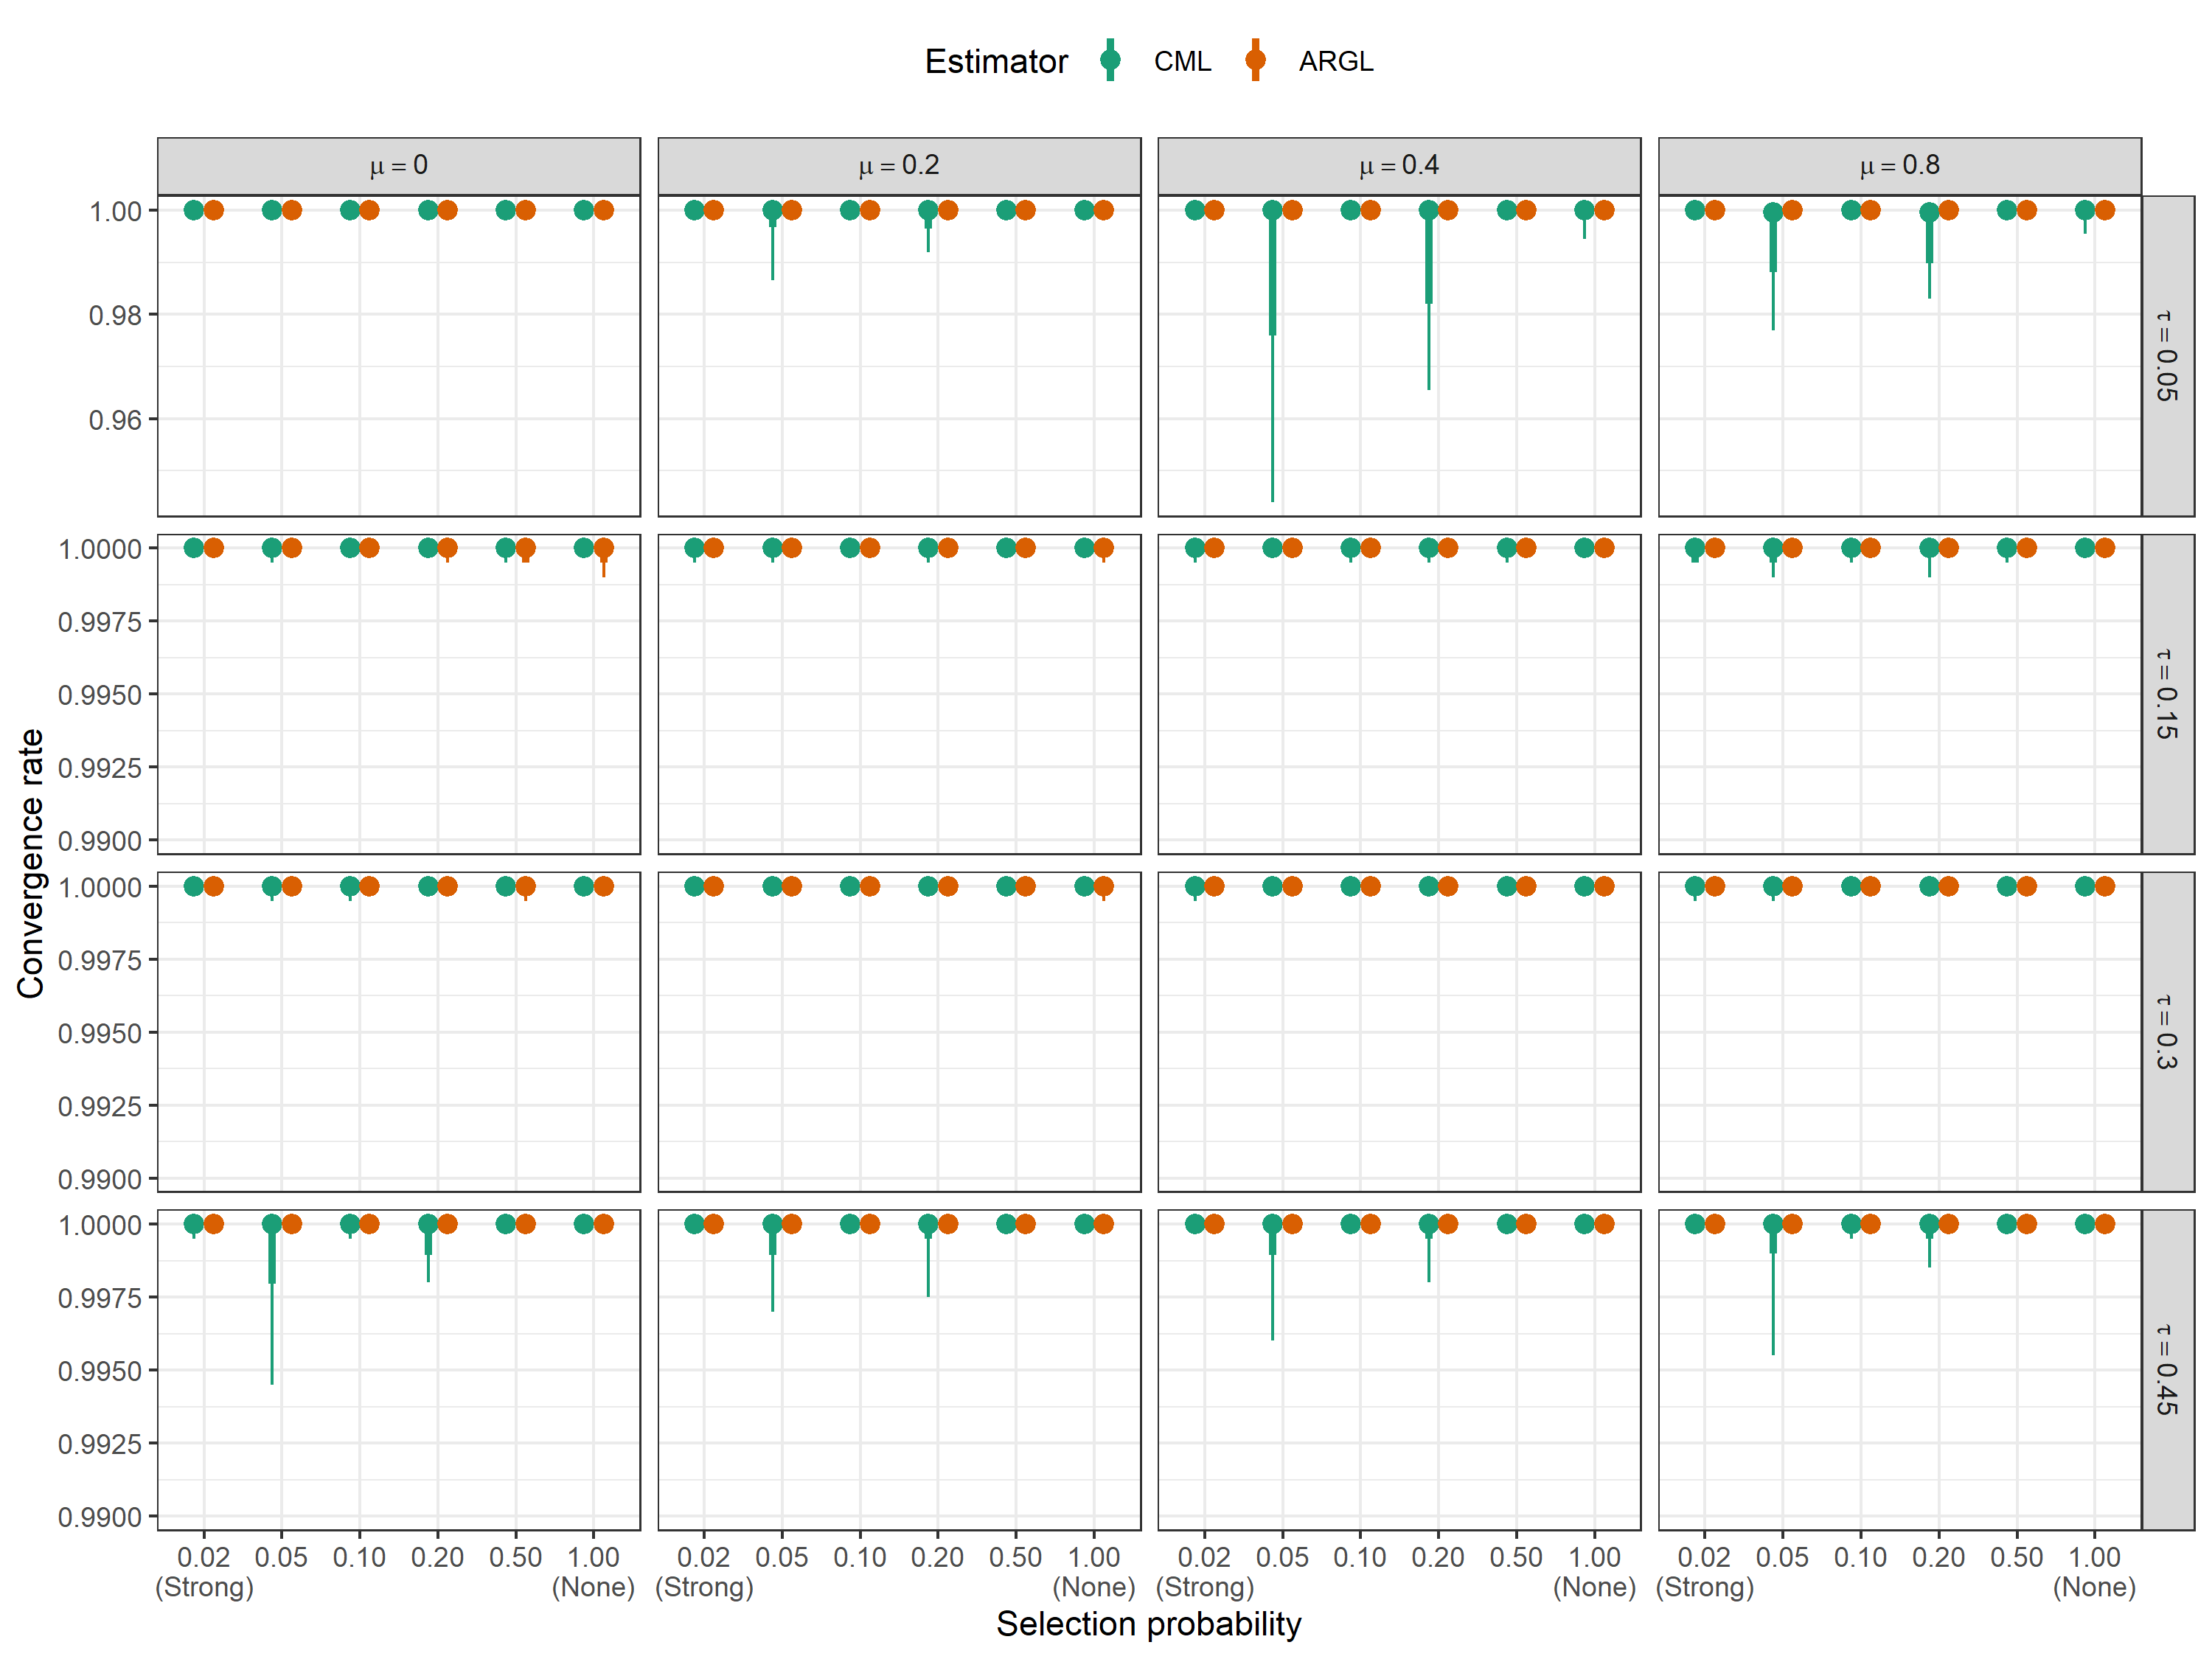
\includegraphics{selection_models_draft_files/figure-latex/convergence-rates-1} \caption{Convergence rates of CML and ARGL estimators by selection probability, average SMD, and between-study heterogeneity. Points correspond to median convergence rates; thin lines correspond to range of convergence rates; thick lines correspond to inter-decile range.}\label{fig:convergence-rates}
\end{sidewaysfigure}

\begin{sidewaysfigure}
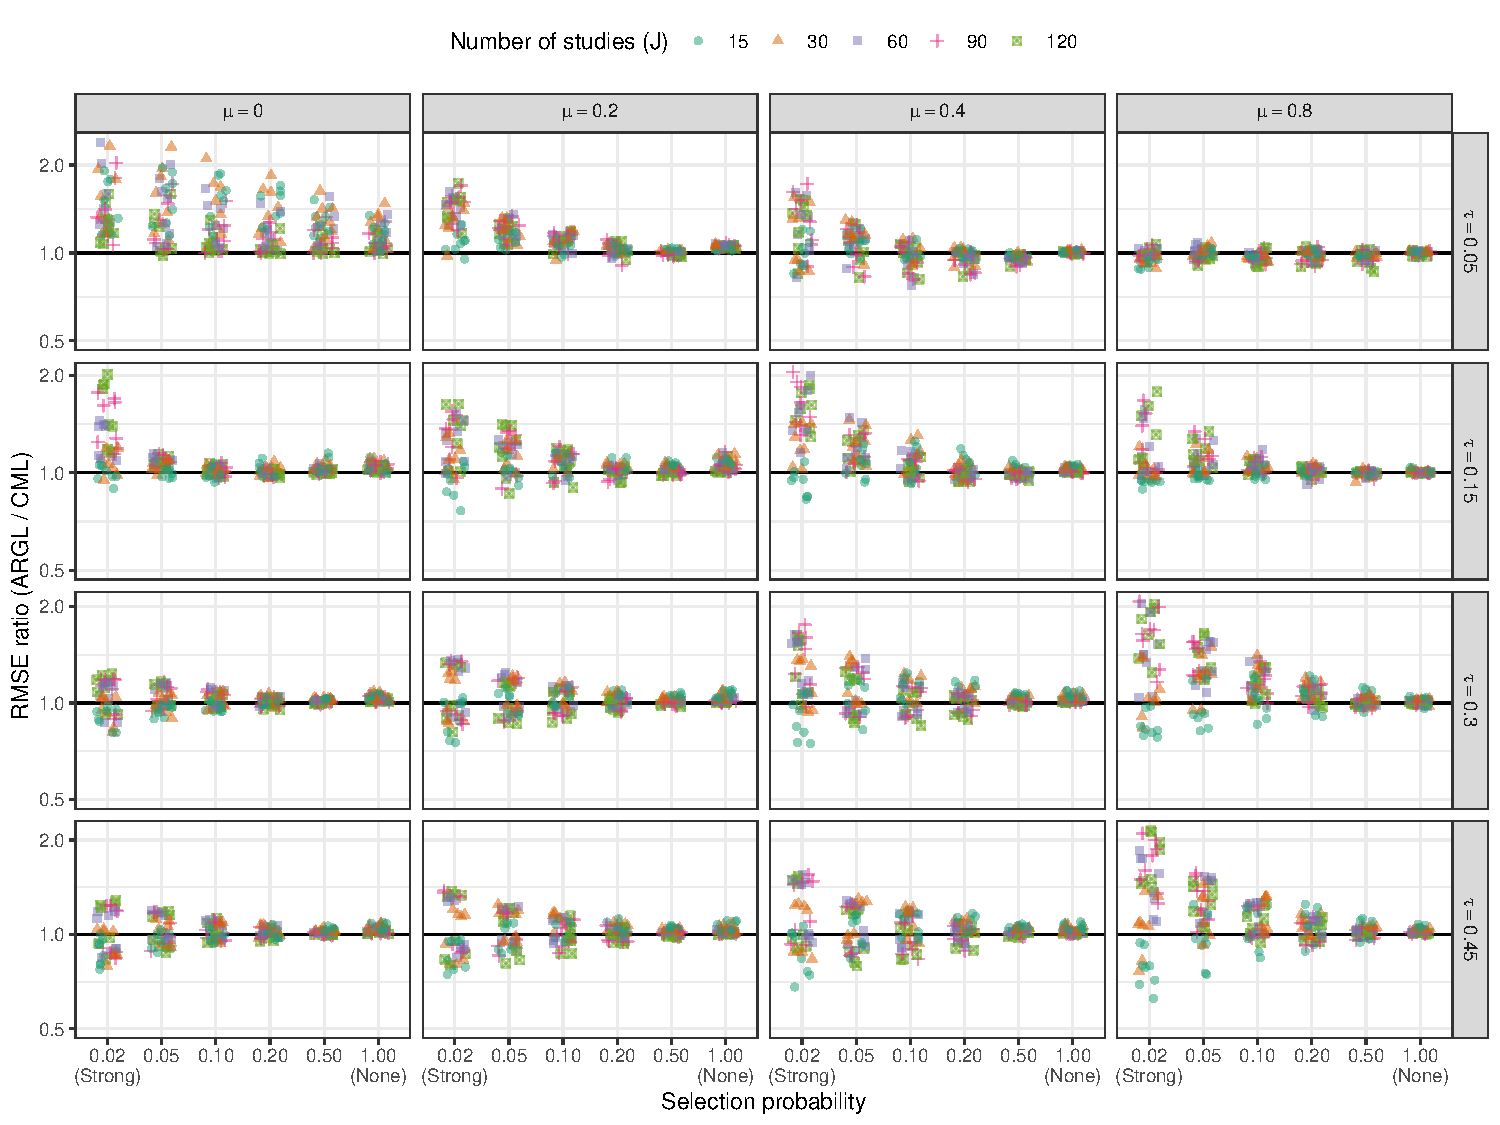
\includegraphics{selection_models_draft_files/figure-latex/rmse-ARGL-CML-1} \caption{Ratio of root mean-squared error for ARGL estimator to root mean-squared error of CML estimator by selection probability, number of studies, average SMD, and between-study heterogeneity}\label{fig:rmse-ARGL-CML}
\end{sidewaysfigure}

\begin{sidewaysfigure}
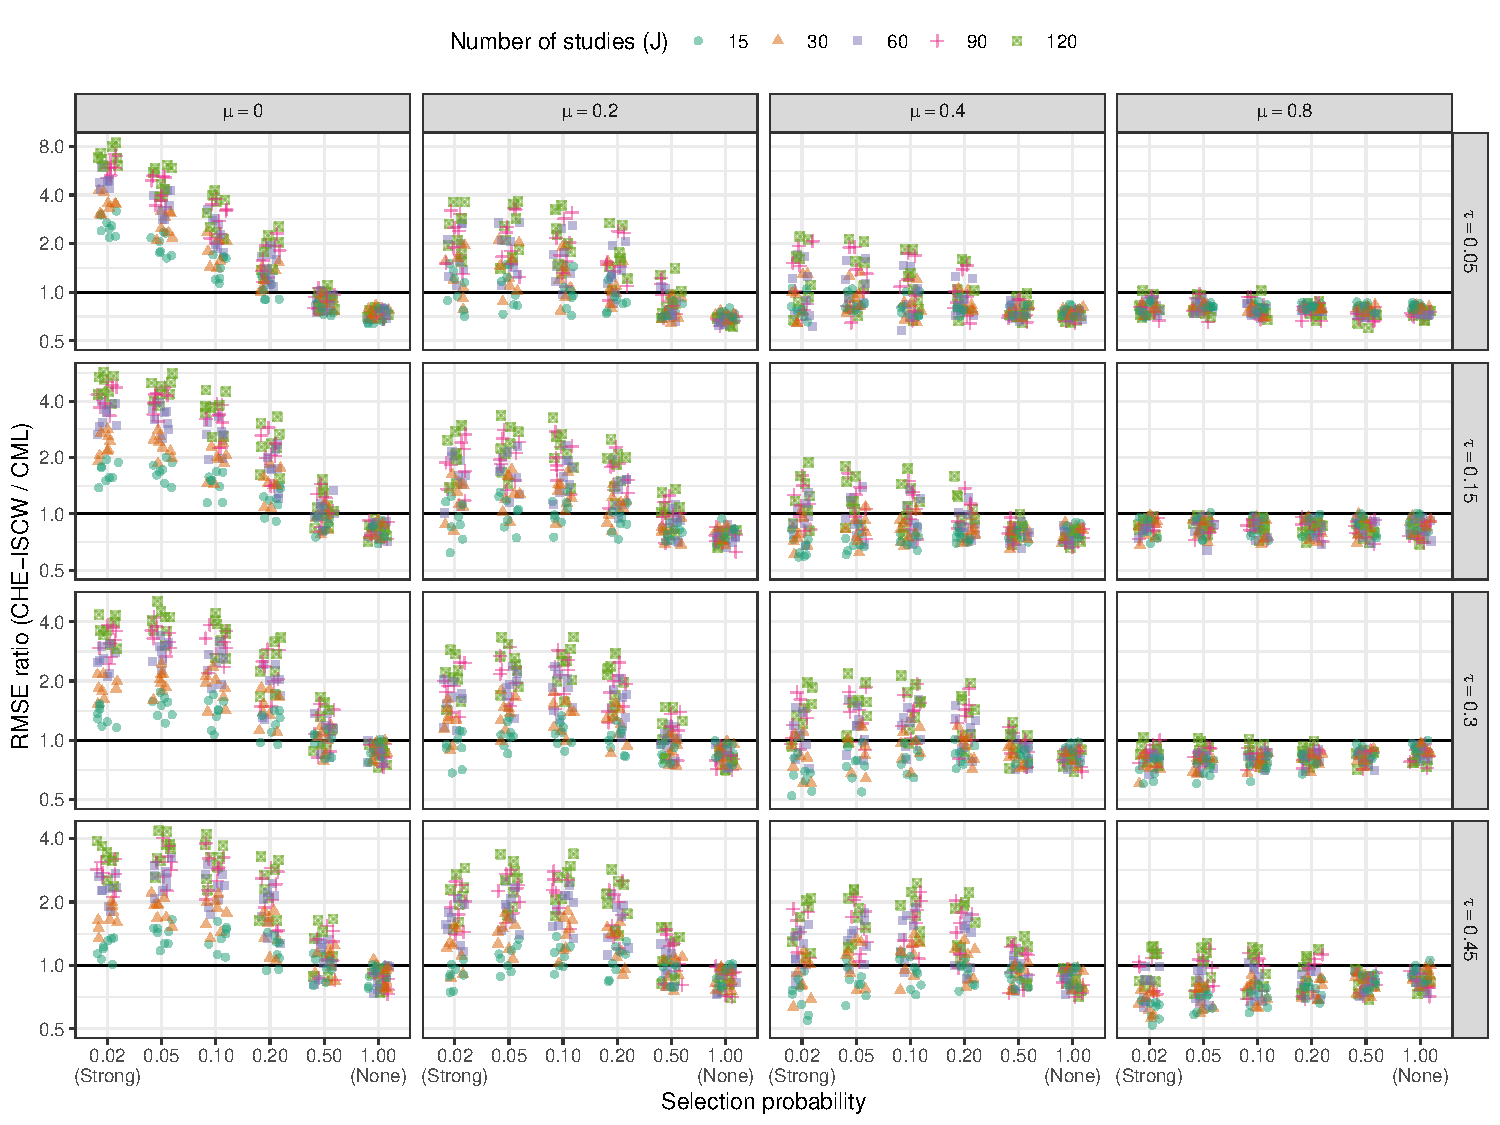
\includegraphics{selection_models_draft_files/figure-latex/rmse-CHE-CML-1} \caption{Ratio of root mean-squared error for CHE-ISCW estimator to root mean-squared error of CML estimator by selection probability, number of studies, average SMD, and between-study heterogeneity}\label{fig:rmse-CHE-CML}
\end{sidewaysfigure}

\begin{sidewaysfigure}
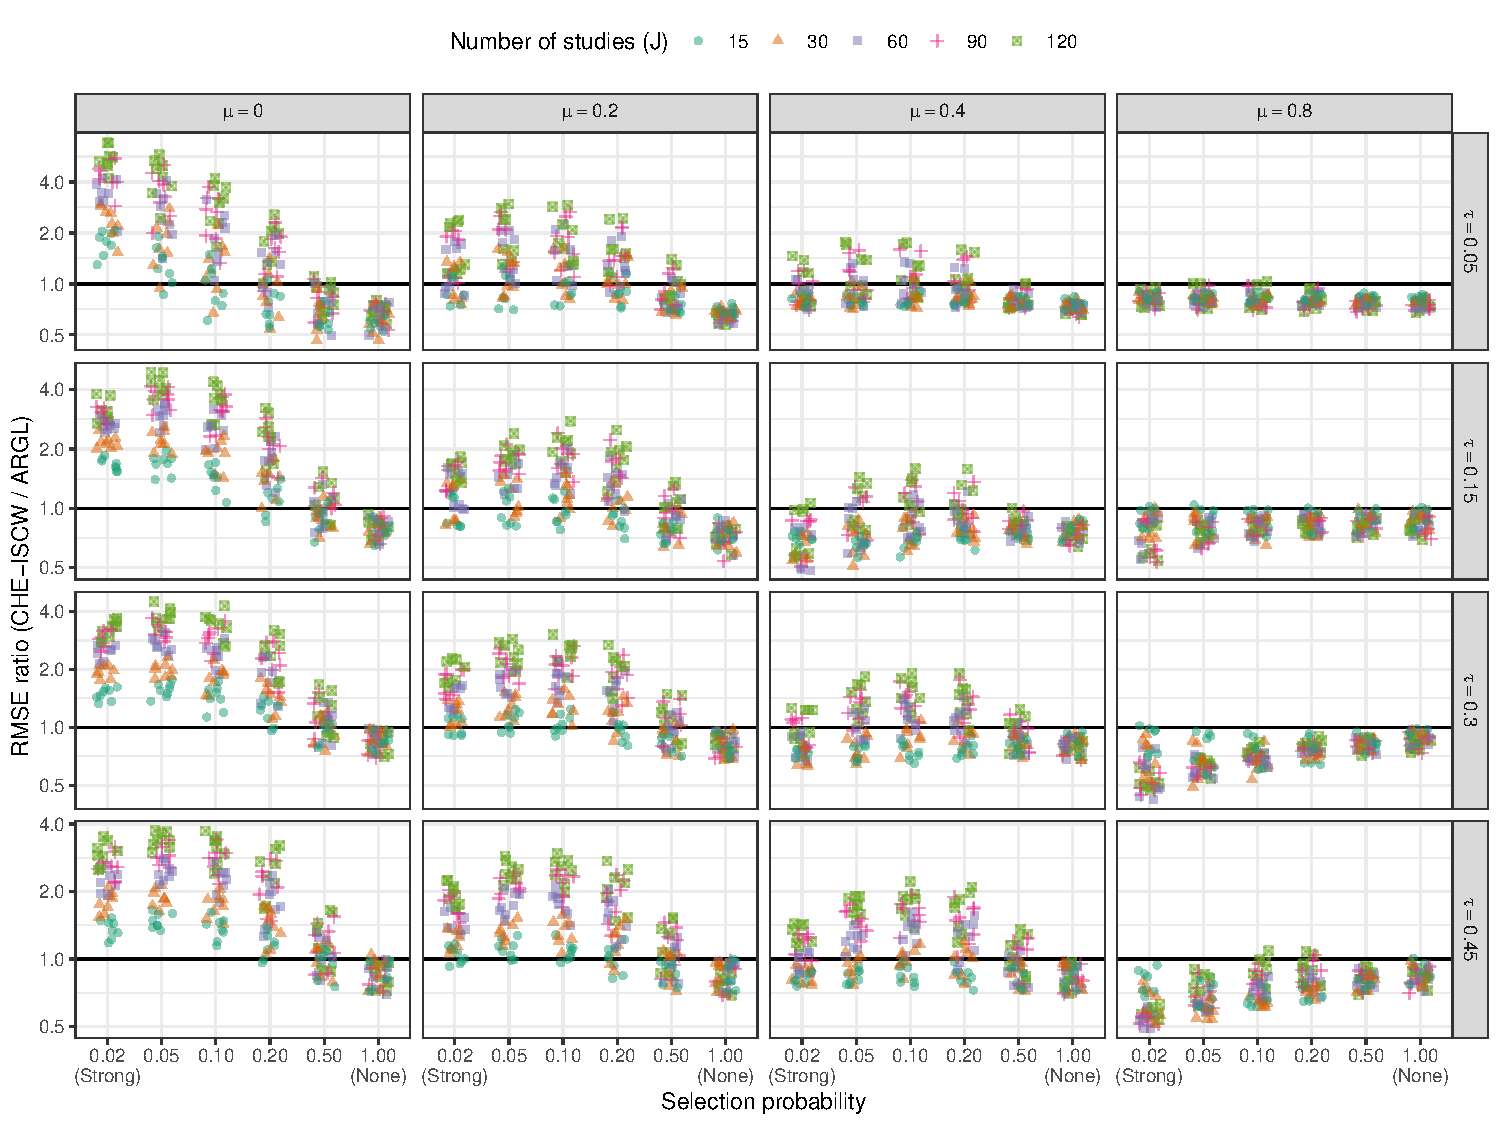
\includegraphics{selection_models_draft_files/figure-latex/rmse-CHE-ARGL-1} \caption{Ratio of root mean-squared error for CHE-ISCW estimator to root mean-squared error of ARGL estimator by selection probability, number of studies, average SMD, and between-study heterogeneity}\label{fig:rmse-CHE-ARGL}
\end{sidewaysfigure}

\begin{sidewaysfigure}
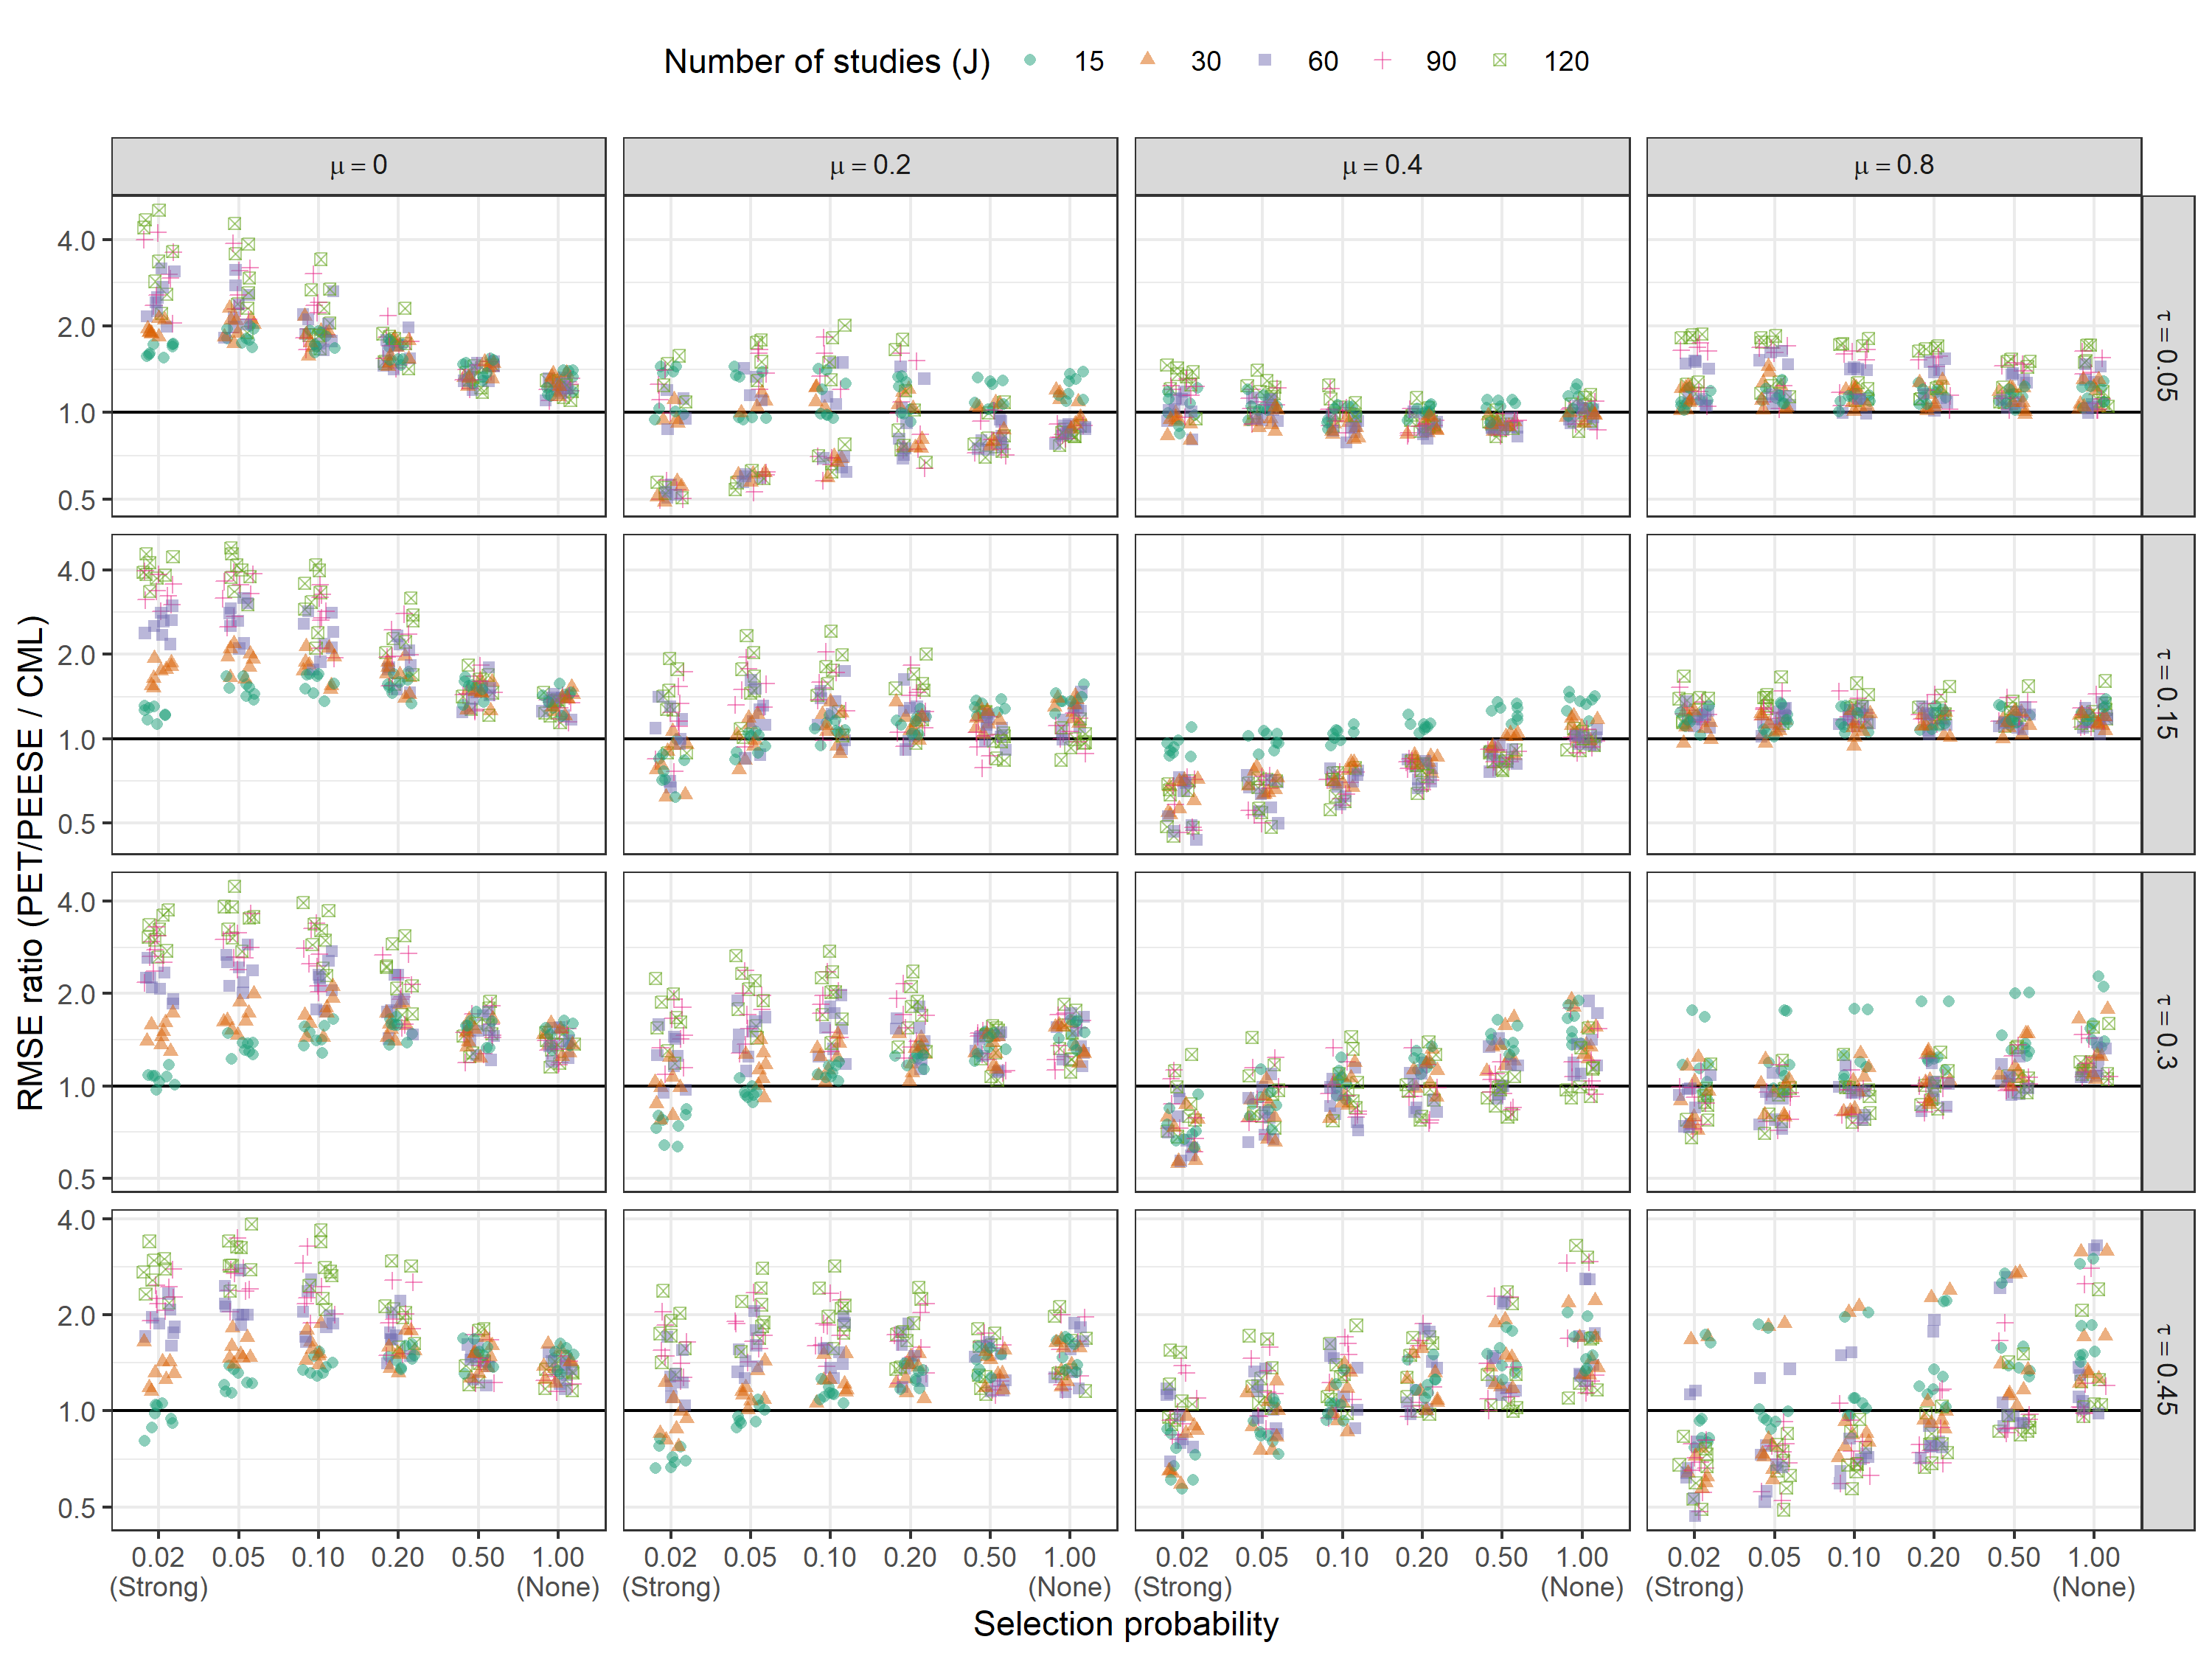
\includegraphics{selection_models_draft_files/figure-latex/rmse-PET-CML-1} \caption{Ratio of root mean-squared error for PET/PEESE estimator to root mean-squared error of CML estimator by selection probability, number of studies, average SMD, and between-study heterogeneity}\label{fig:rmse-PET-CML}
\end{sidewaysfigure}

\begin{sidewaysfigure}
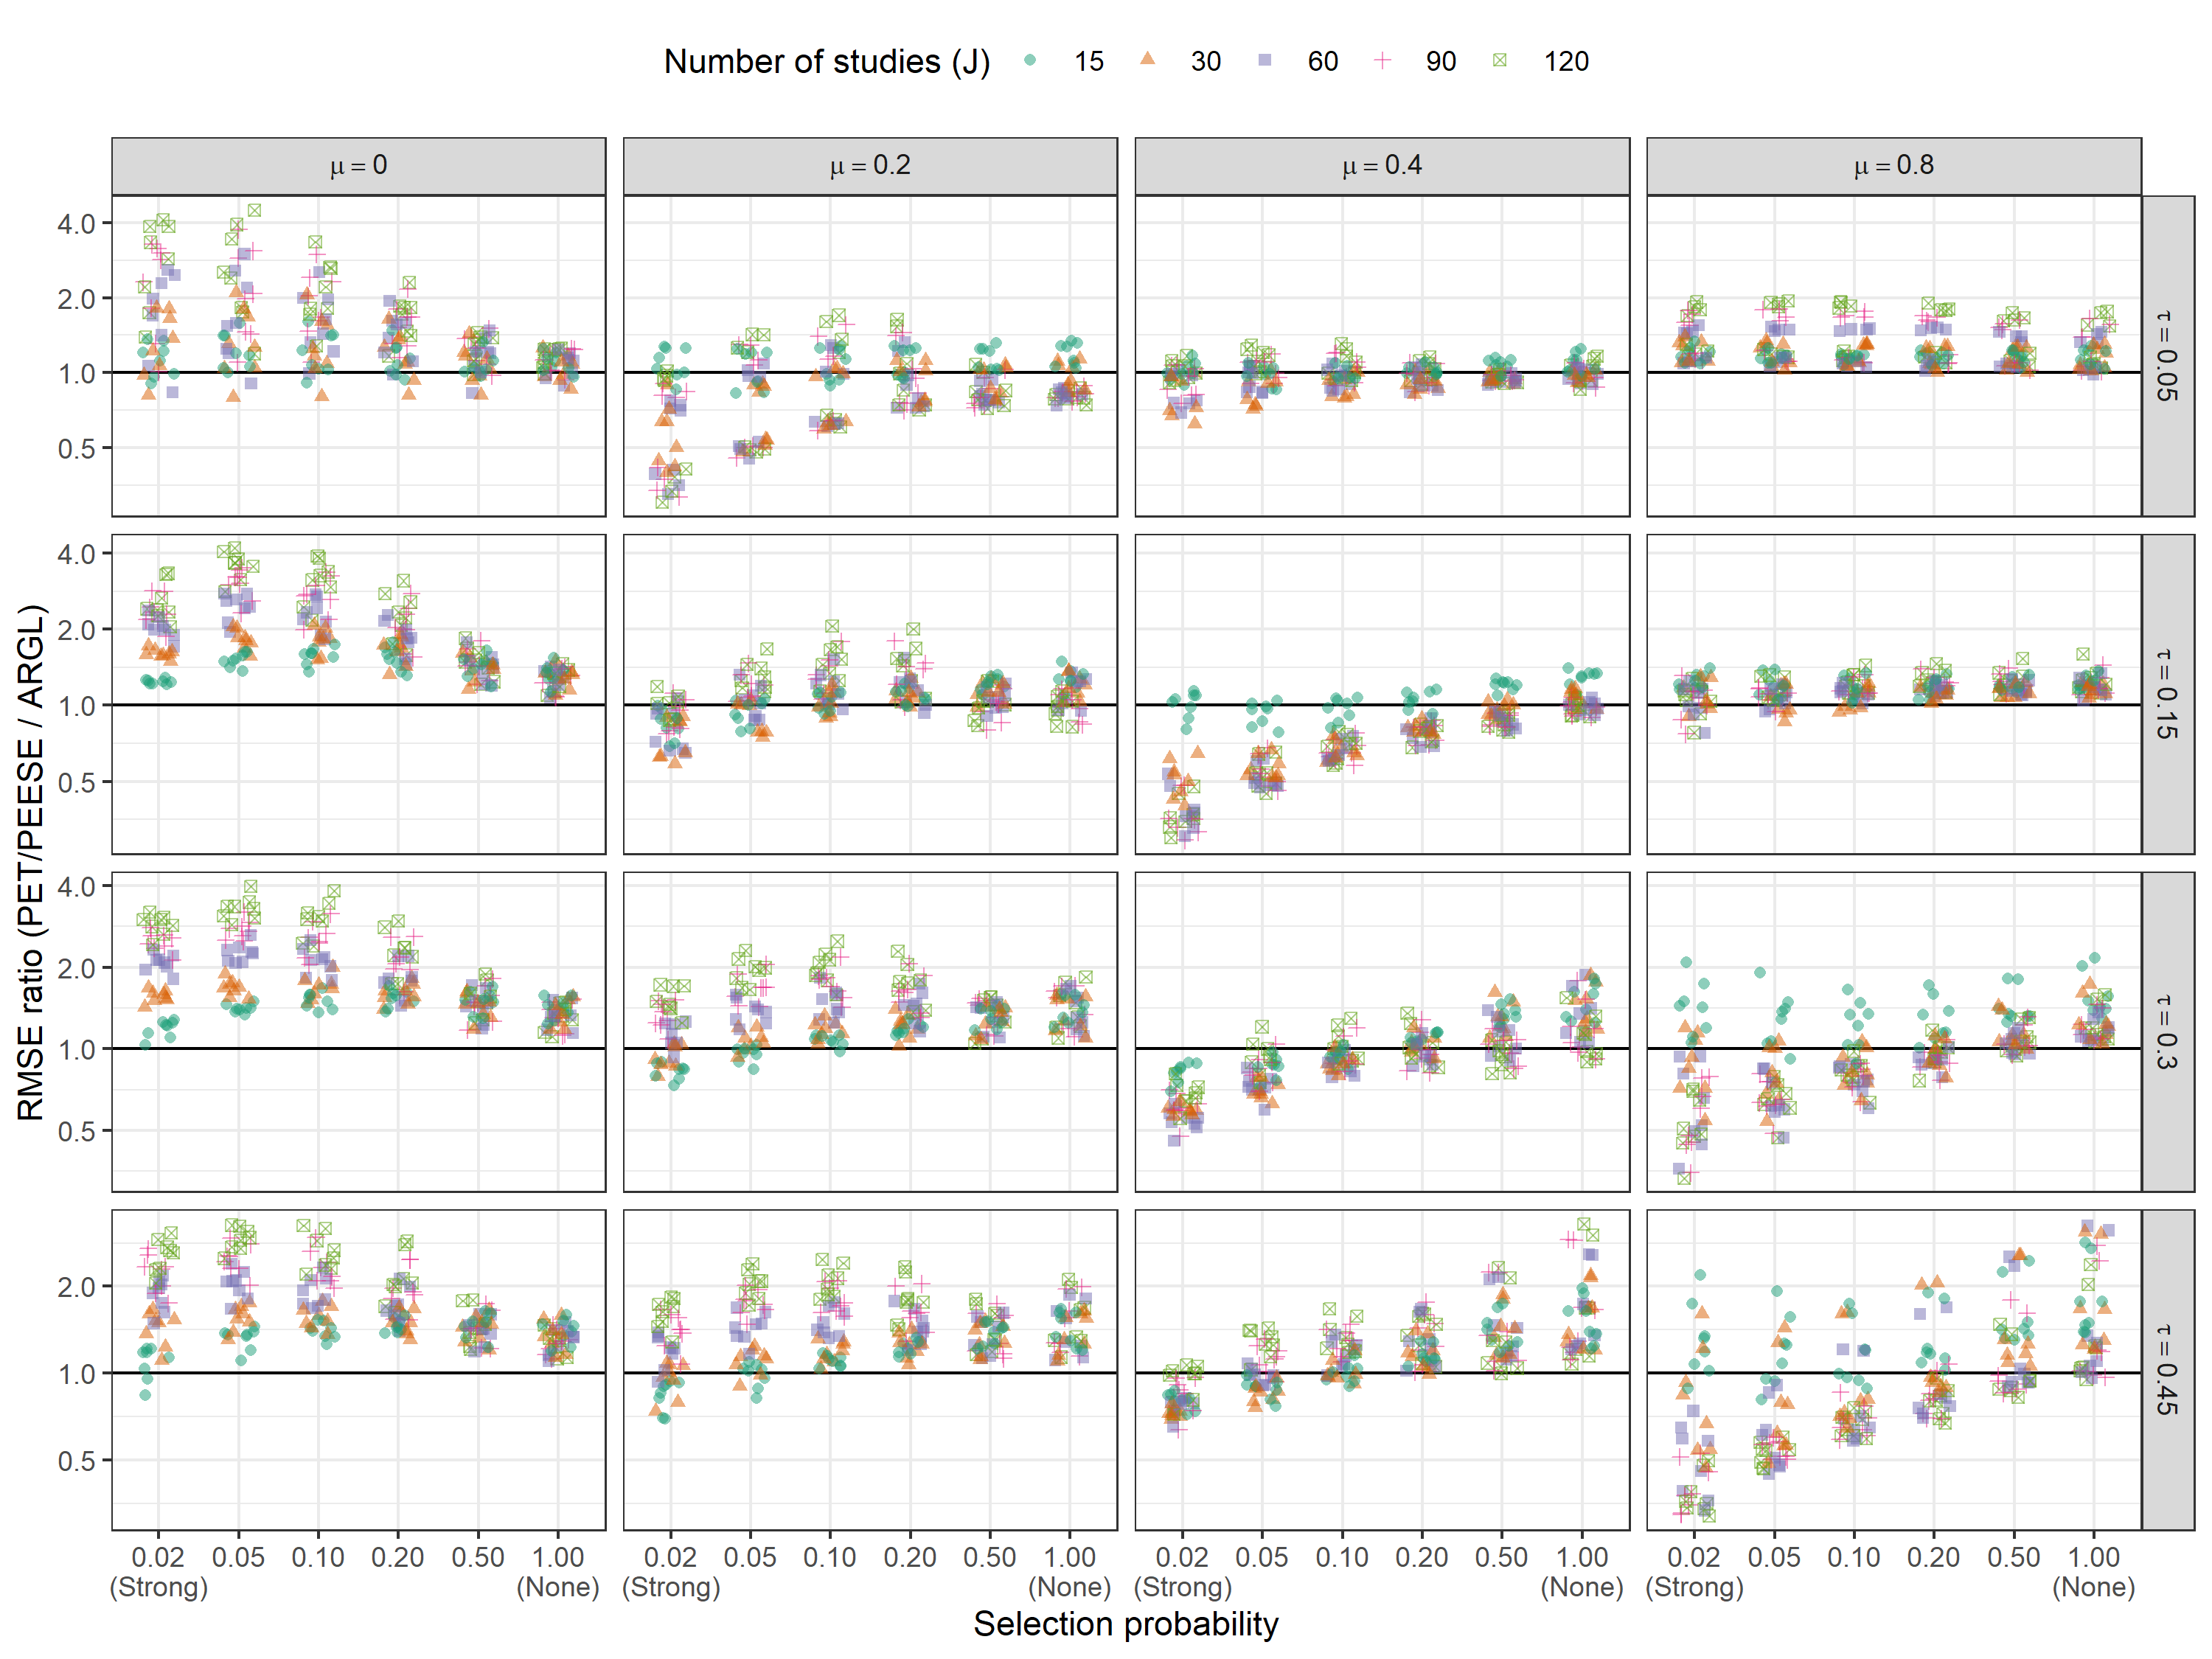
\includegraphics{selection_models_draft_files/figure-latex/rmse-PET-ARGL-1} \caption{Ratio of root mean-squared error for PET/PEESE estimator to root mean-squared error of ARGL estimator by selection probability, number of studies, average SMD, and between-study heterogeneity}\label{fig:rmse-PET-ARGL}
\end{sidewaysfigure}

\begin{sidewaysfigure}
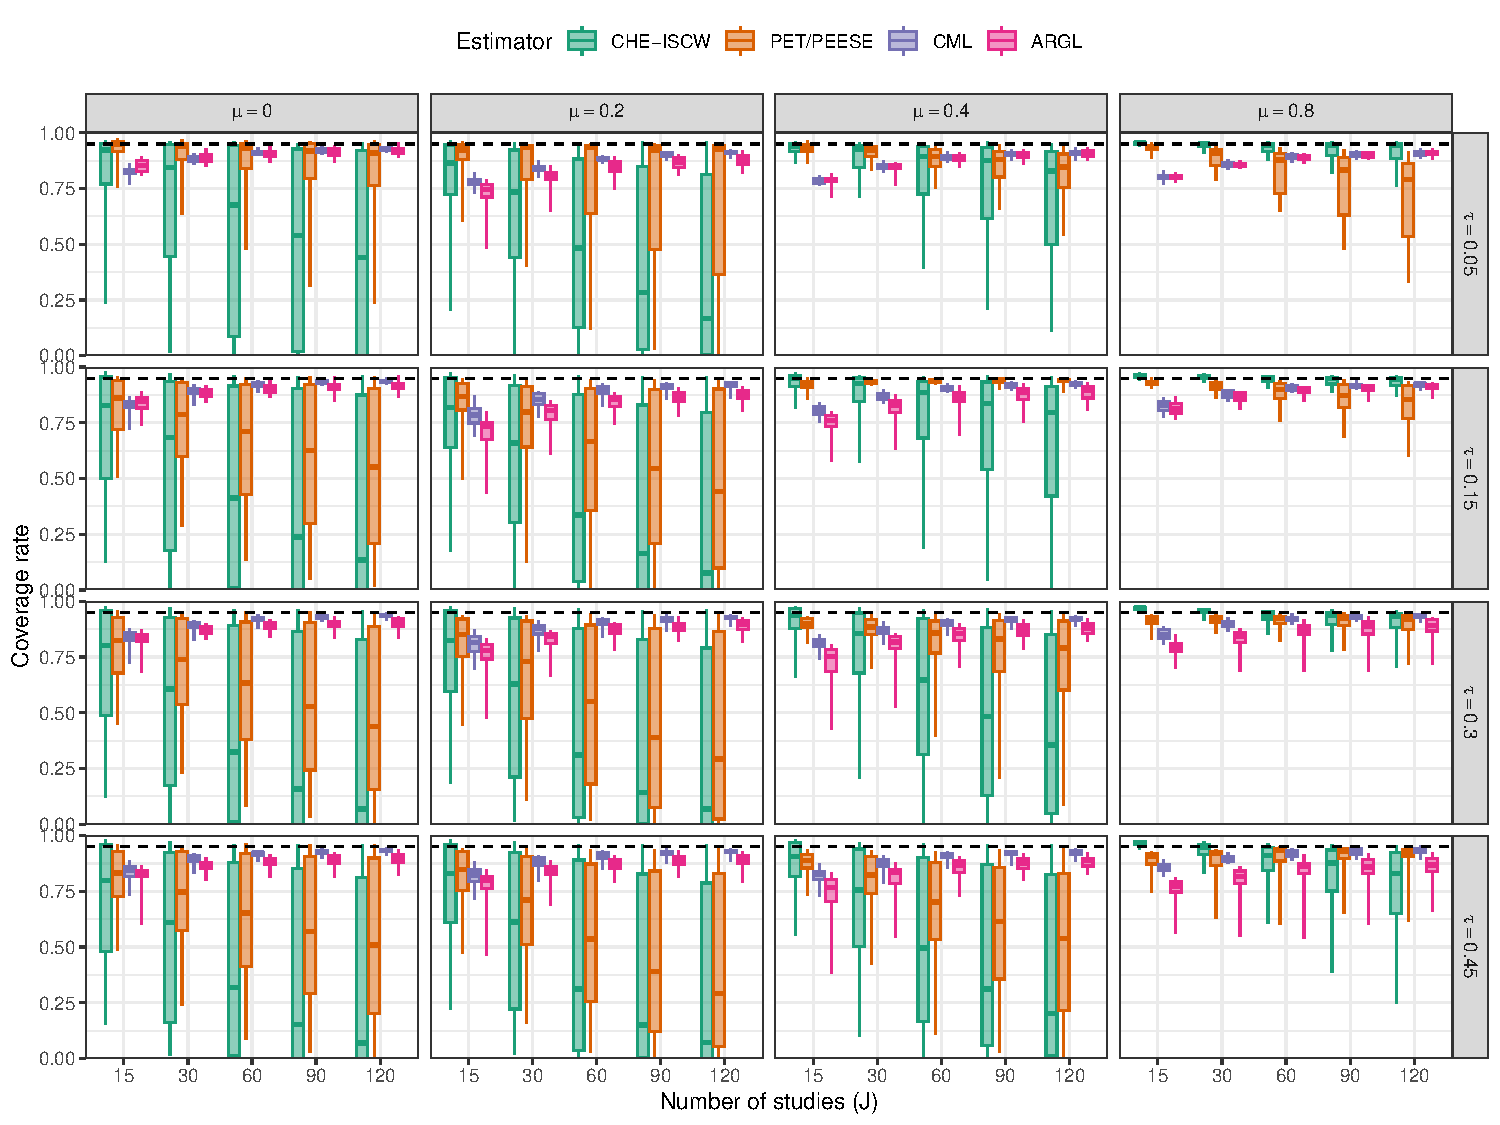
\includegraphics{selection_models_draft_files/figure-latex/comparison-coverage-full-1} \caption{Coverage levels of confidence intervals based for average effect size based on cluster-robust variance approximations, by number of studies, average SMD, and between-study heterogeneity. Dashed lines correspond to the nominal confidence level of 0.95.}\label{fig:comparison-coverage-full}
\end{sidewaysfigure}

\begin{sidewaysfigure}
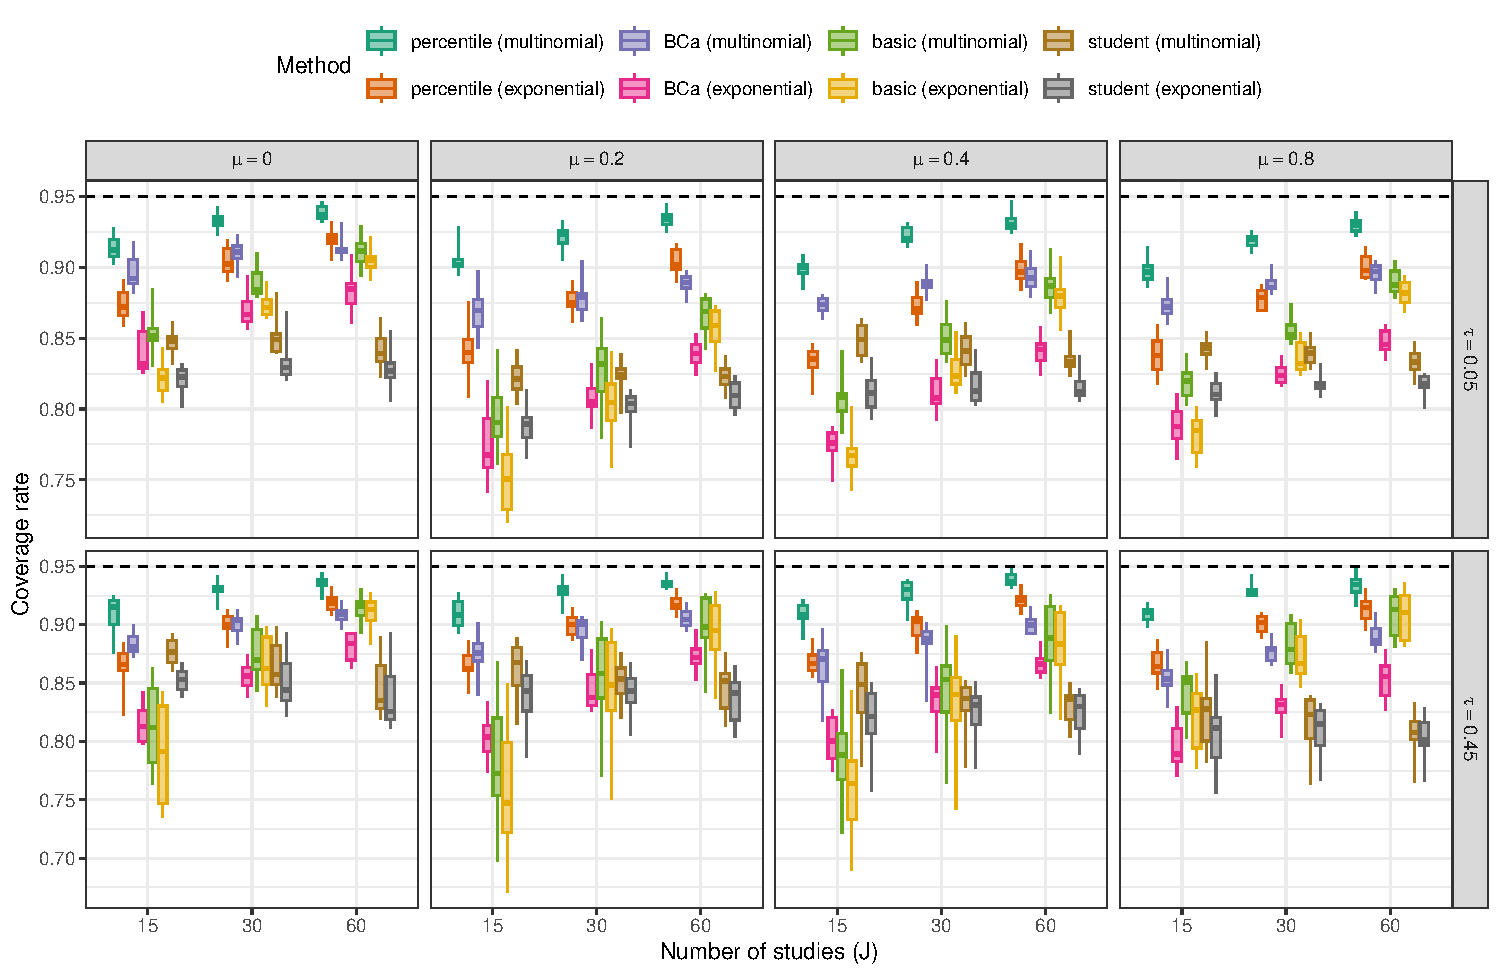
\includegraphics{selection_models_draft_files/figure-latex/CML-coverage-full-1} \caption{Coverage levels of bootstrap confidence intervals based on the CML estimator of average effect size by number of studies, average SMD, and between-study heterogeneity. Dashed lines correspond to the nominal confidence level of 0.95.}\label{fig:CML-coverage-full}
\end{sidewaysfigure}

\begin{sidewaysfigure}
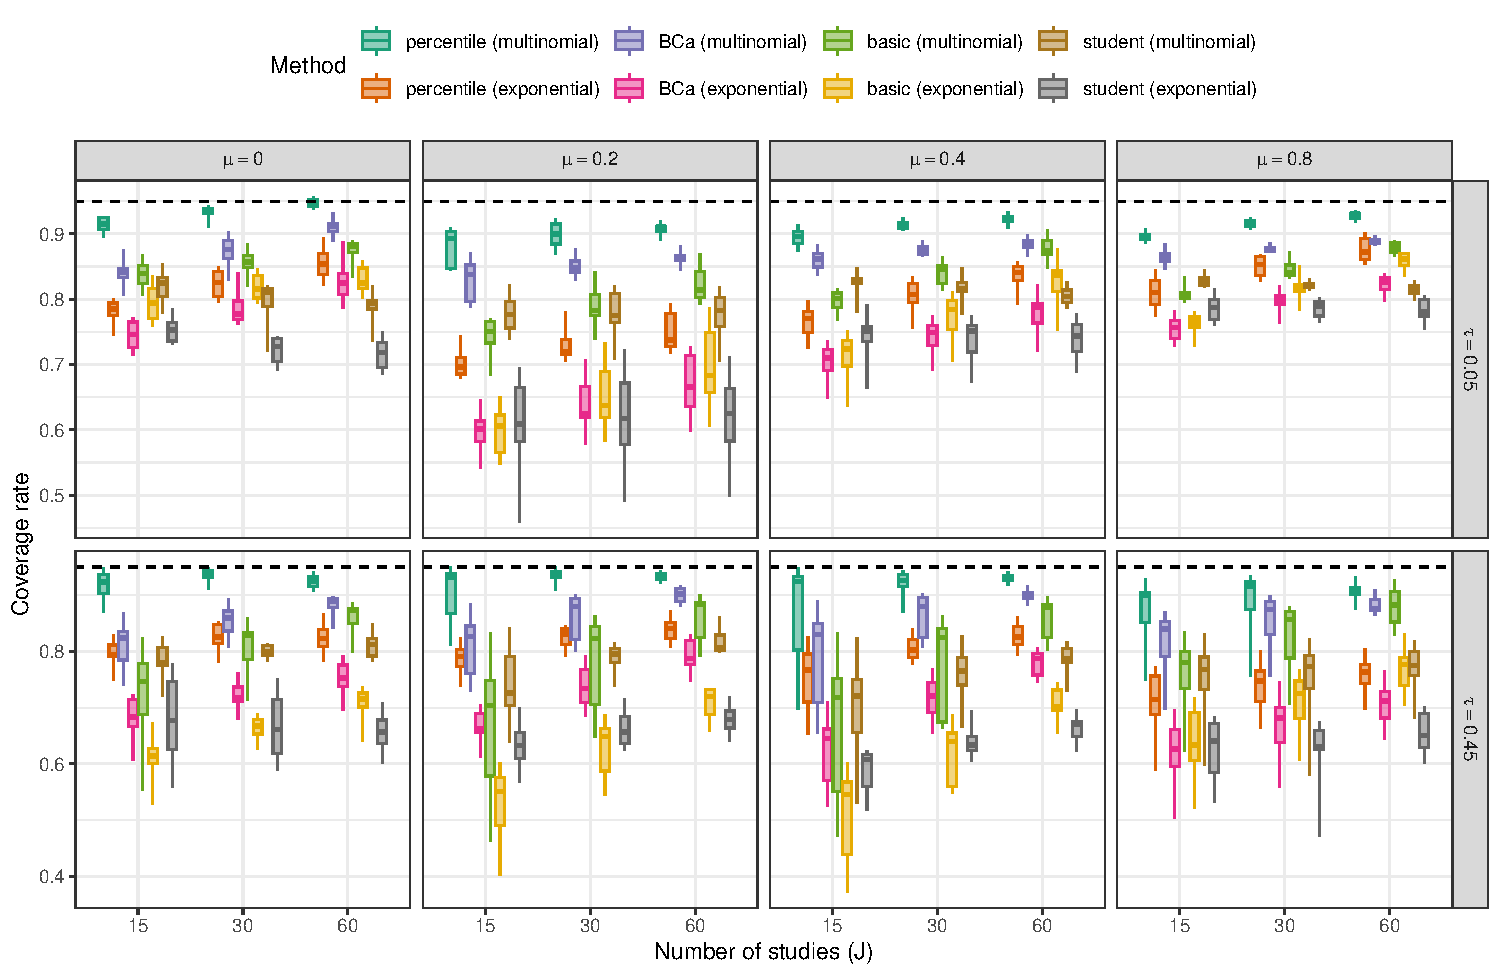
\includegraphics{selection_models_draft_files/figure-latex/ARGL-coverage-full-1} \caption{Coverage levels of bootstrap confidence intervals based on the ARGL estimator of average effect size by number of studies, average SMD, and between-study heterogeneity. Dashed lines correspond to the nominal confidence level of 0.95.}\label{fig:ARGL-coverage-full}
\end{sidewaysfigure}

\section{\texorpdfstring{Additional simulation results for estimators of log-heterogeneity \((\gamma)\)}{Additional simulation results for estimators of log-heterogeneity (\textbackslash gamma)}}\label{gamma-simulation-results}

\begin{sidewaysfigure}
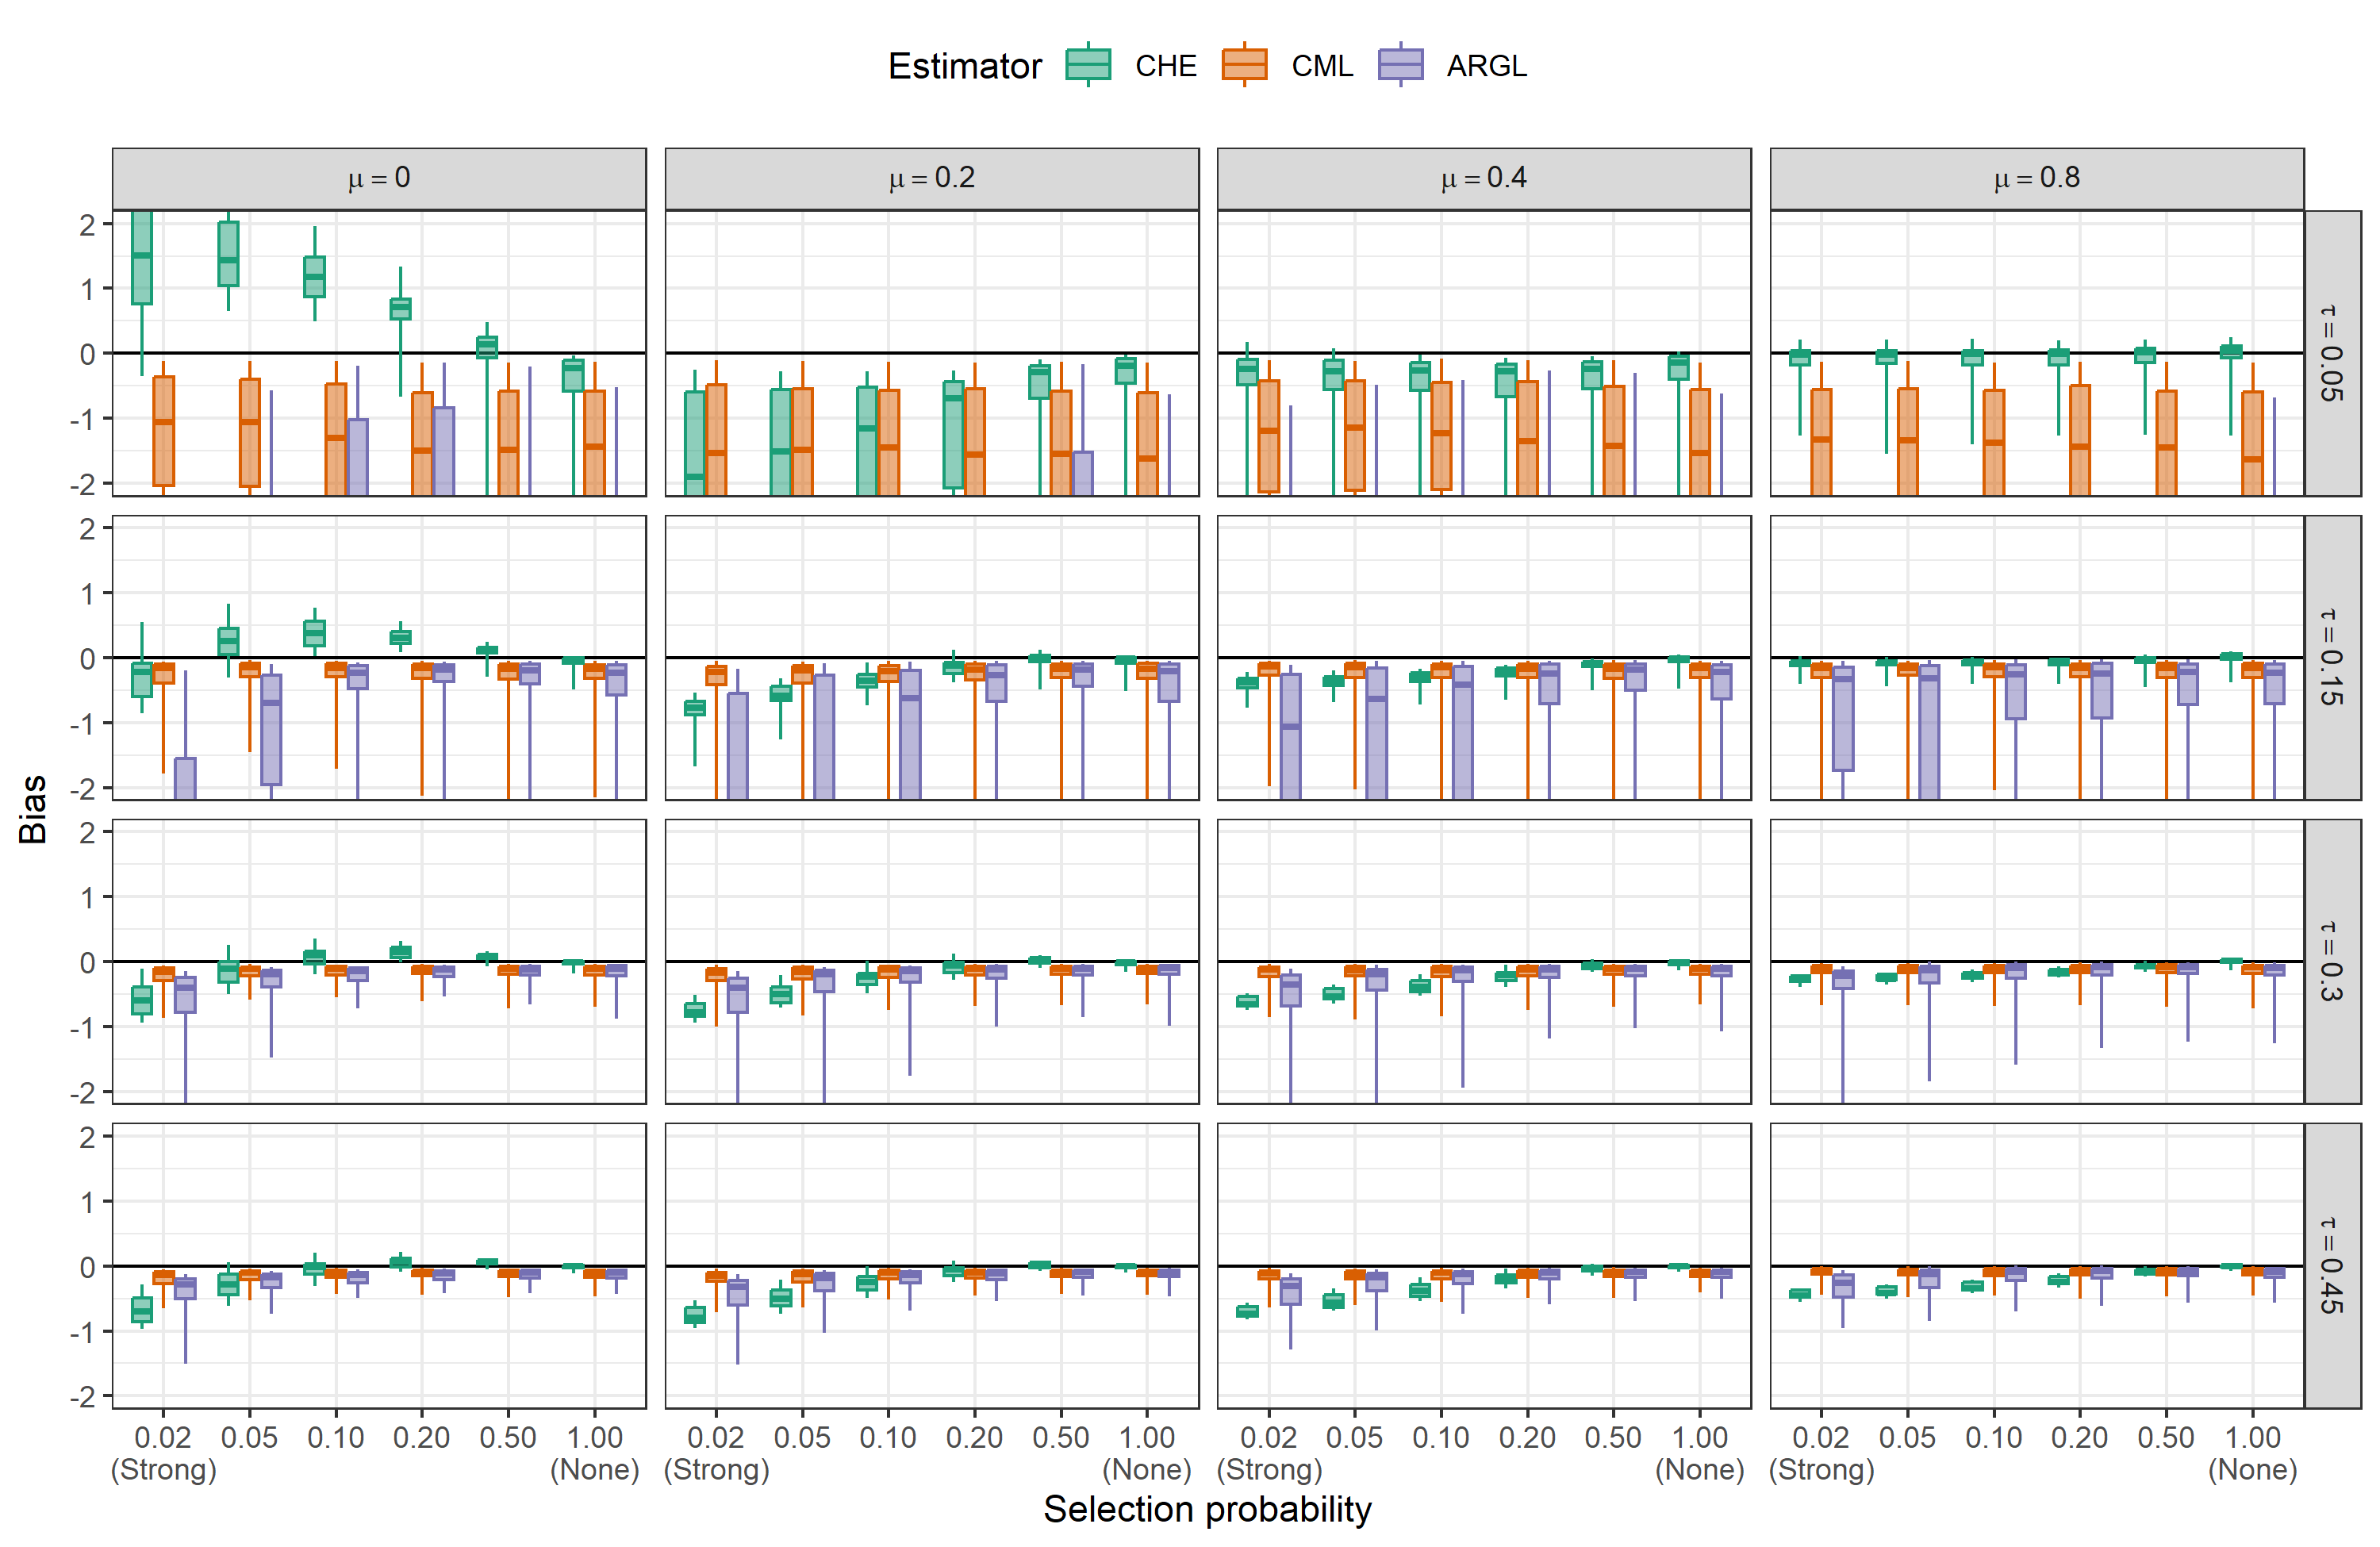
\includegraphics{selection_models_draft_files/figure-latex/heterogeneity-bias-1} \caption{Bias for estimators of log-heterogeneity by selection probability, average SMD, and between-study heterogeneity}\label{fig:heterogeneity-bias}
\end{sidewaysfigure}

\begin{sidewaysfigure}
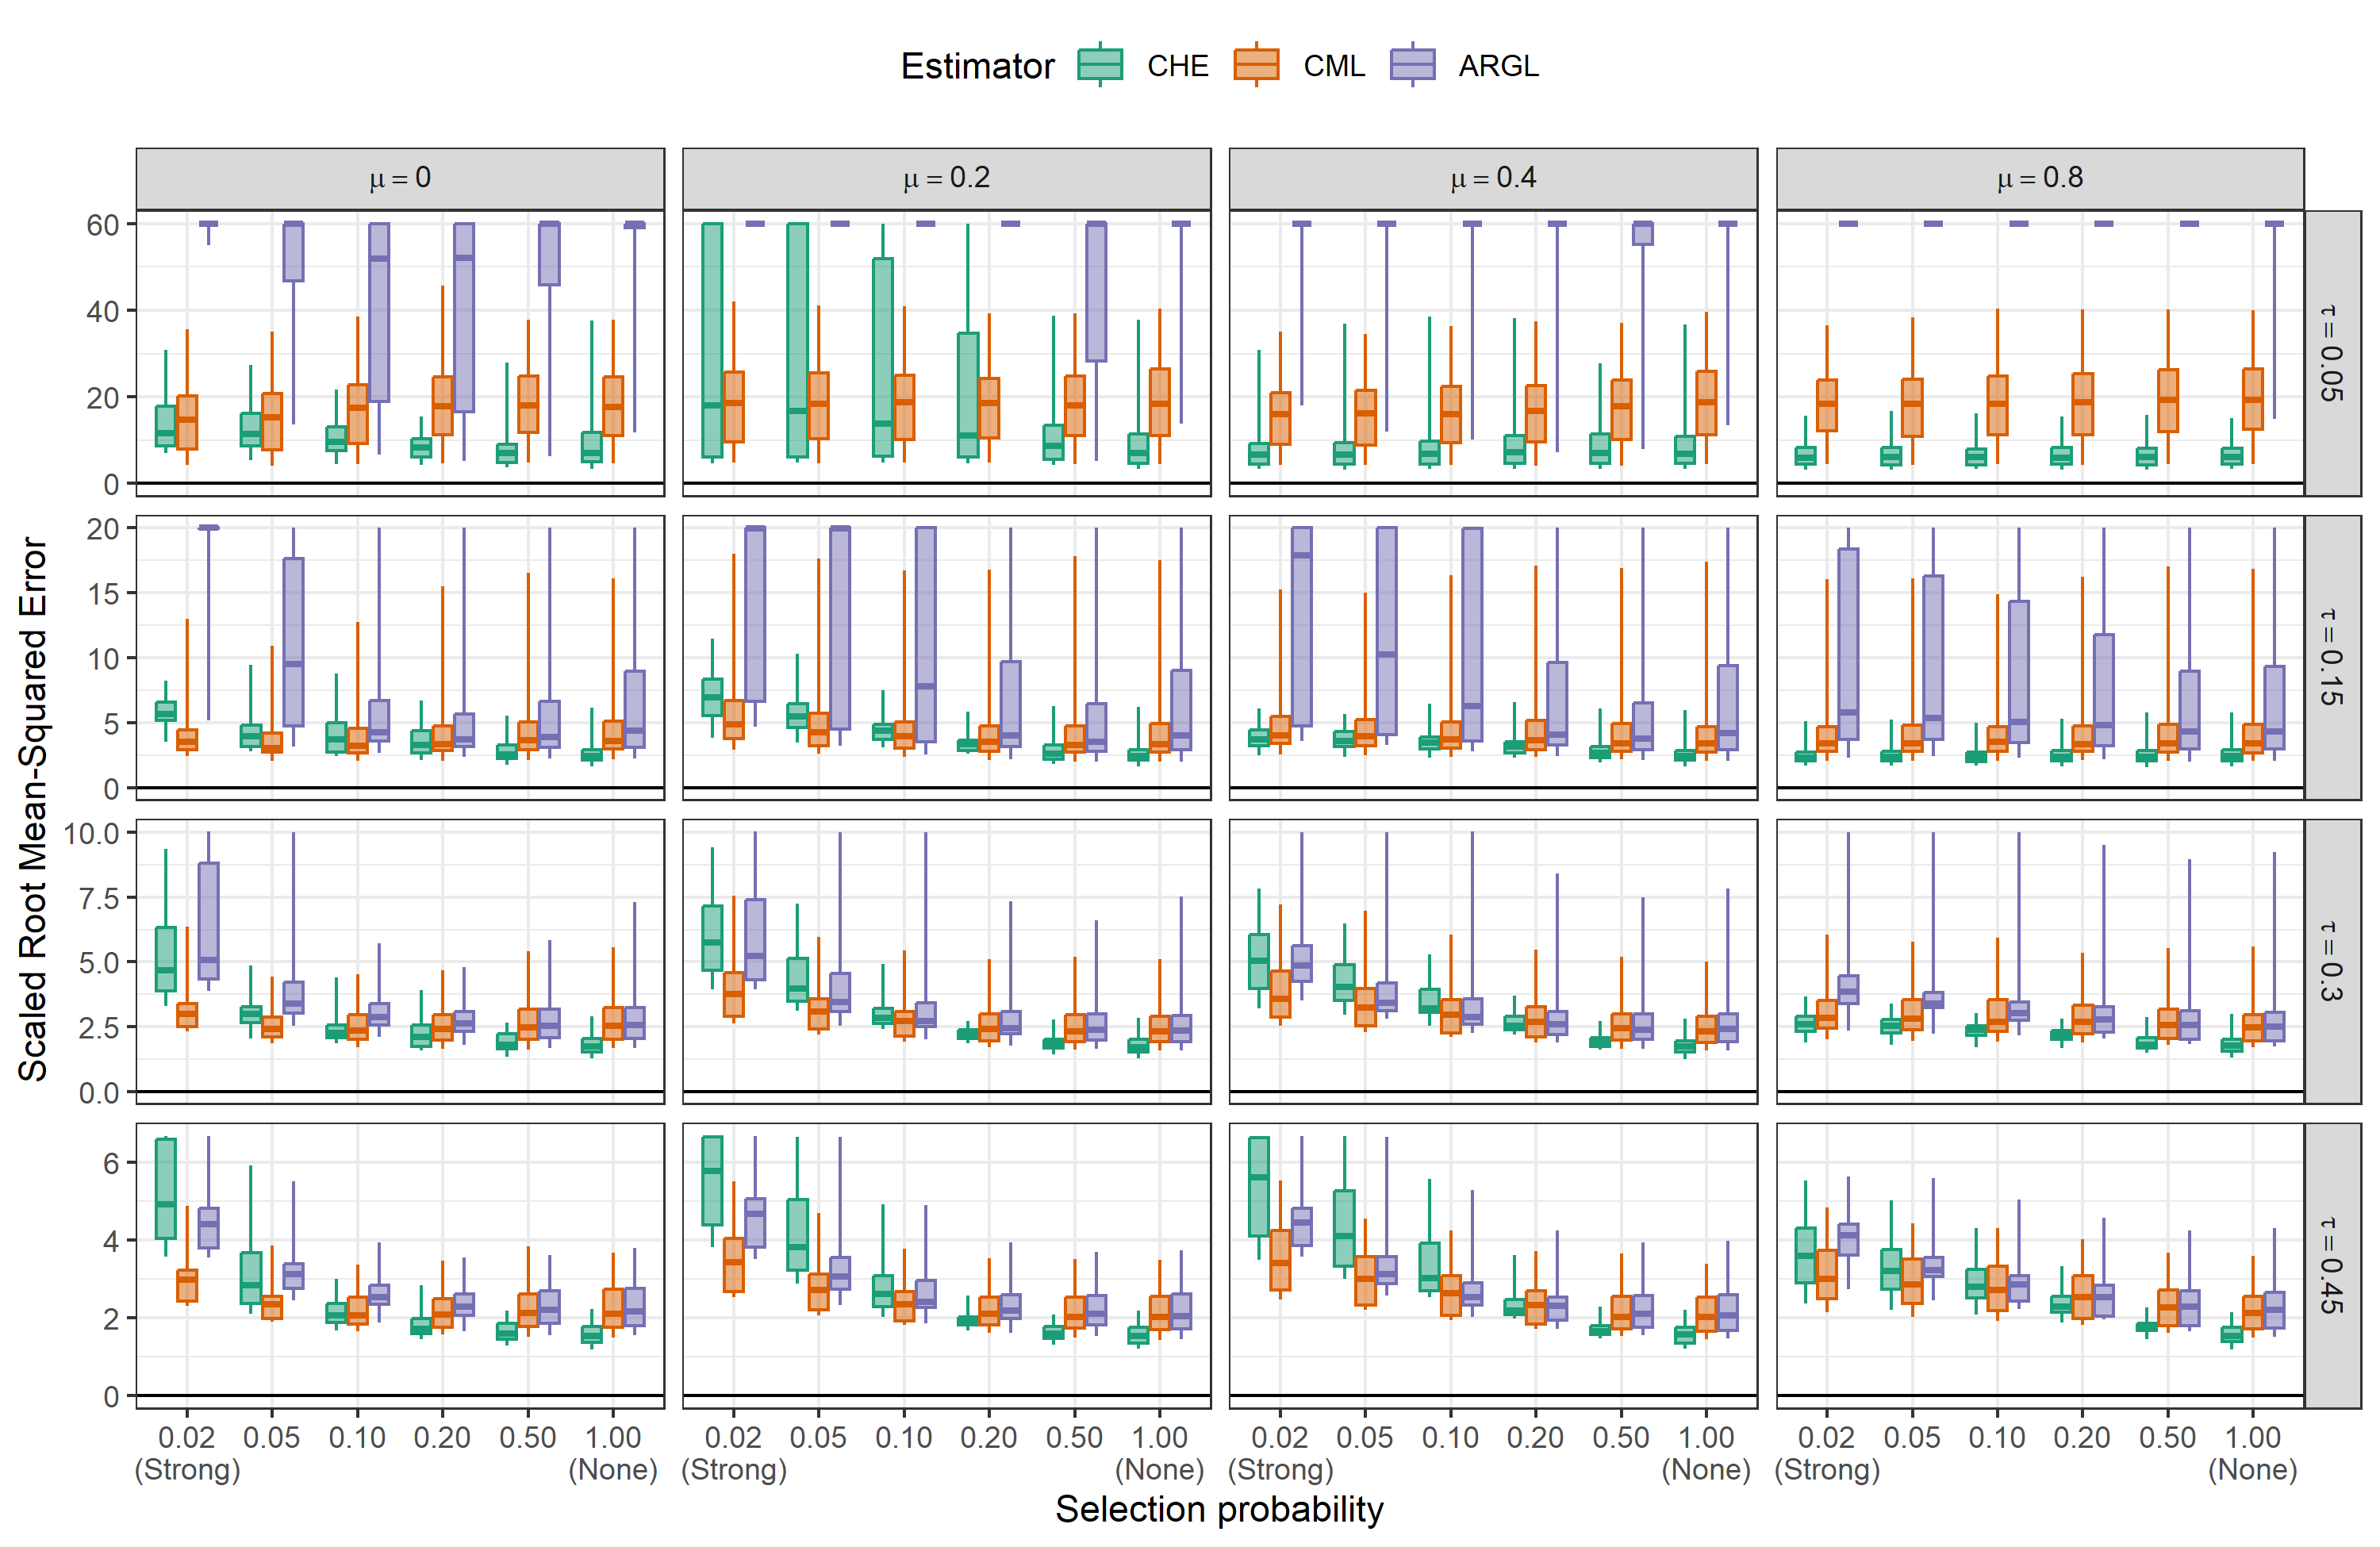
\includegraphics{selection_models_draft_files/figure-latex/heterogeneity-rmse-1} \caption{Scaled root mean-squared error for estimators of log-heterogeneity by selection probability, average SMD, and between-study heterogeneity}\label{fig:heterogeneity-rmse}
\end{sidewaysfigure}
\begin{sidewaysfigure}
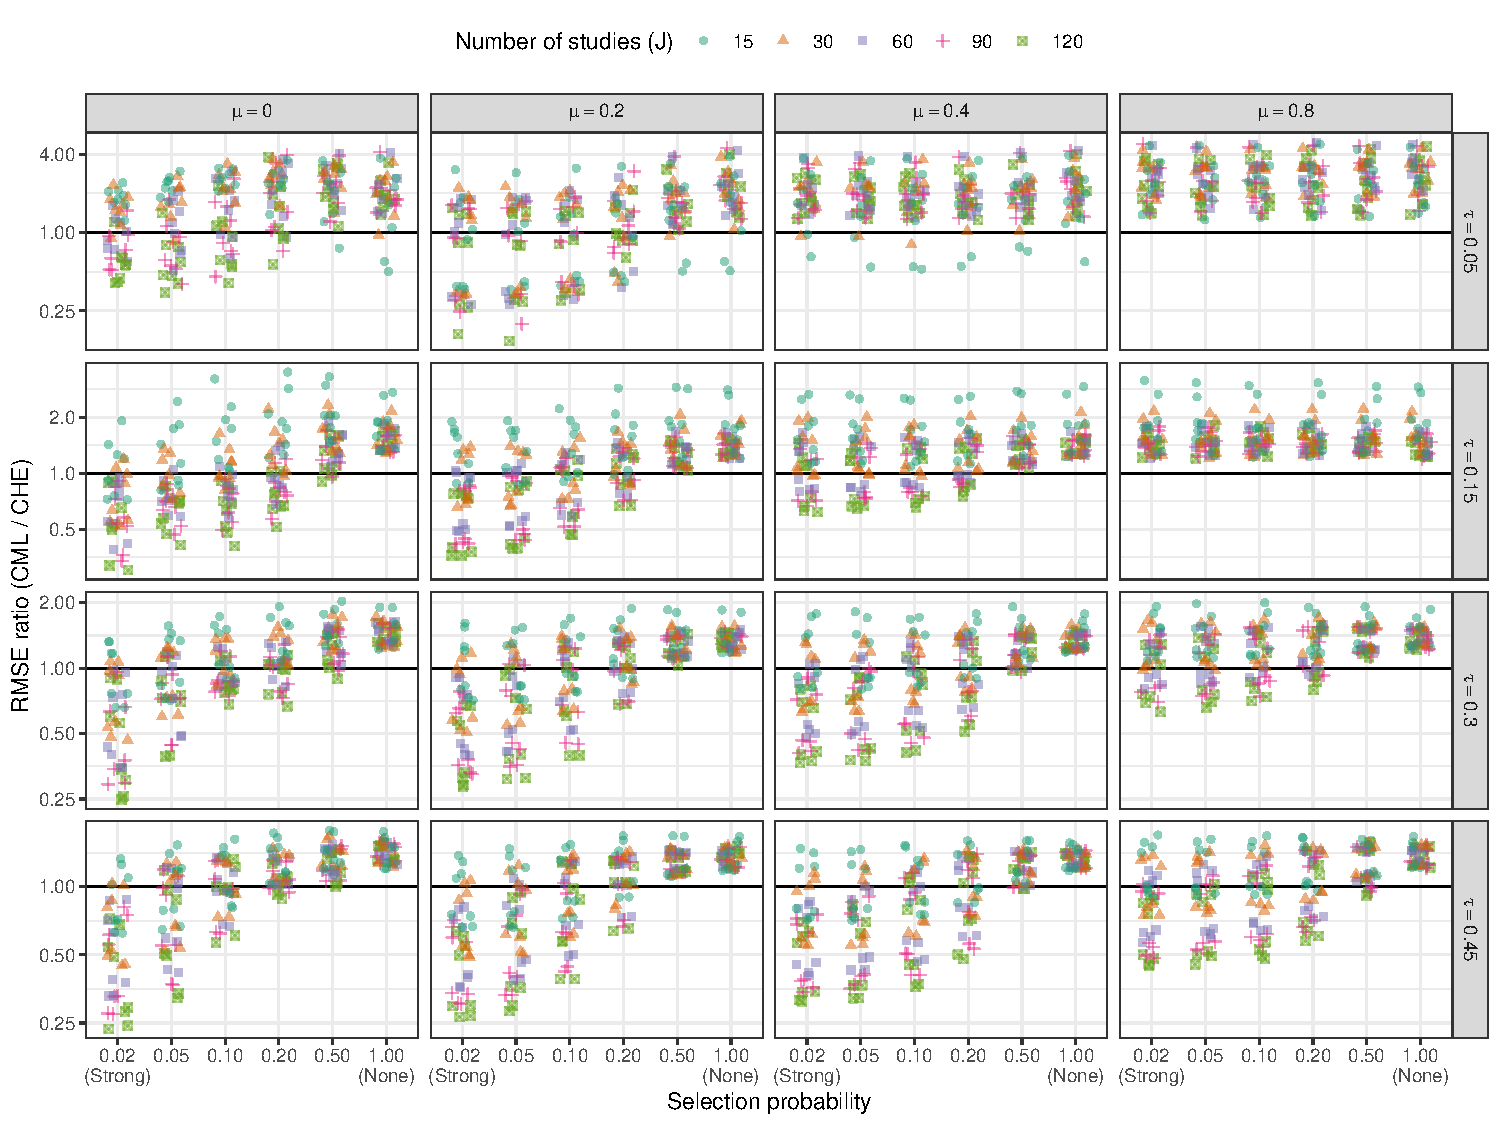
\includegraphics{selection_models_draft_files/figure-latex/heterogeneity-rmse-CML-CHE-1} \caption{Ratio of root mean-squared error for CML heterogeneity estimator to root mean-squared error of CHE heterogeneity estimator by selection probability, number of studies, average SMD, and between-study heterogeneity}\label{fig:heterogeneity-rmse-CML-CHE}
\end{sidewaysfigure}

\begin{sidewaysfigure}
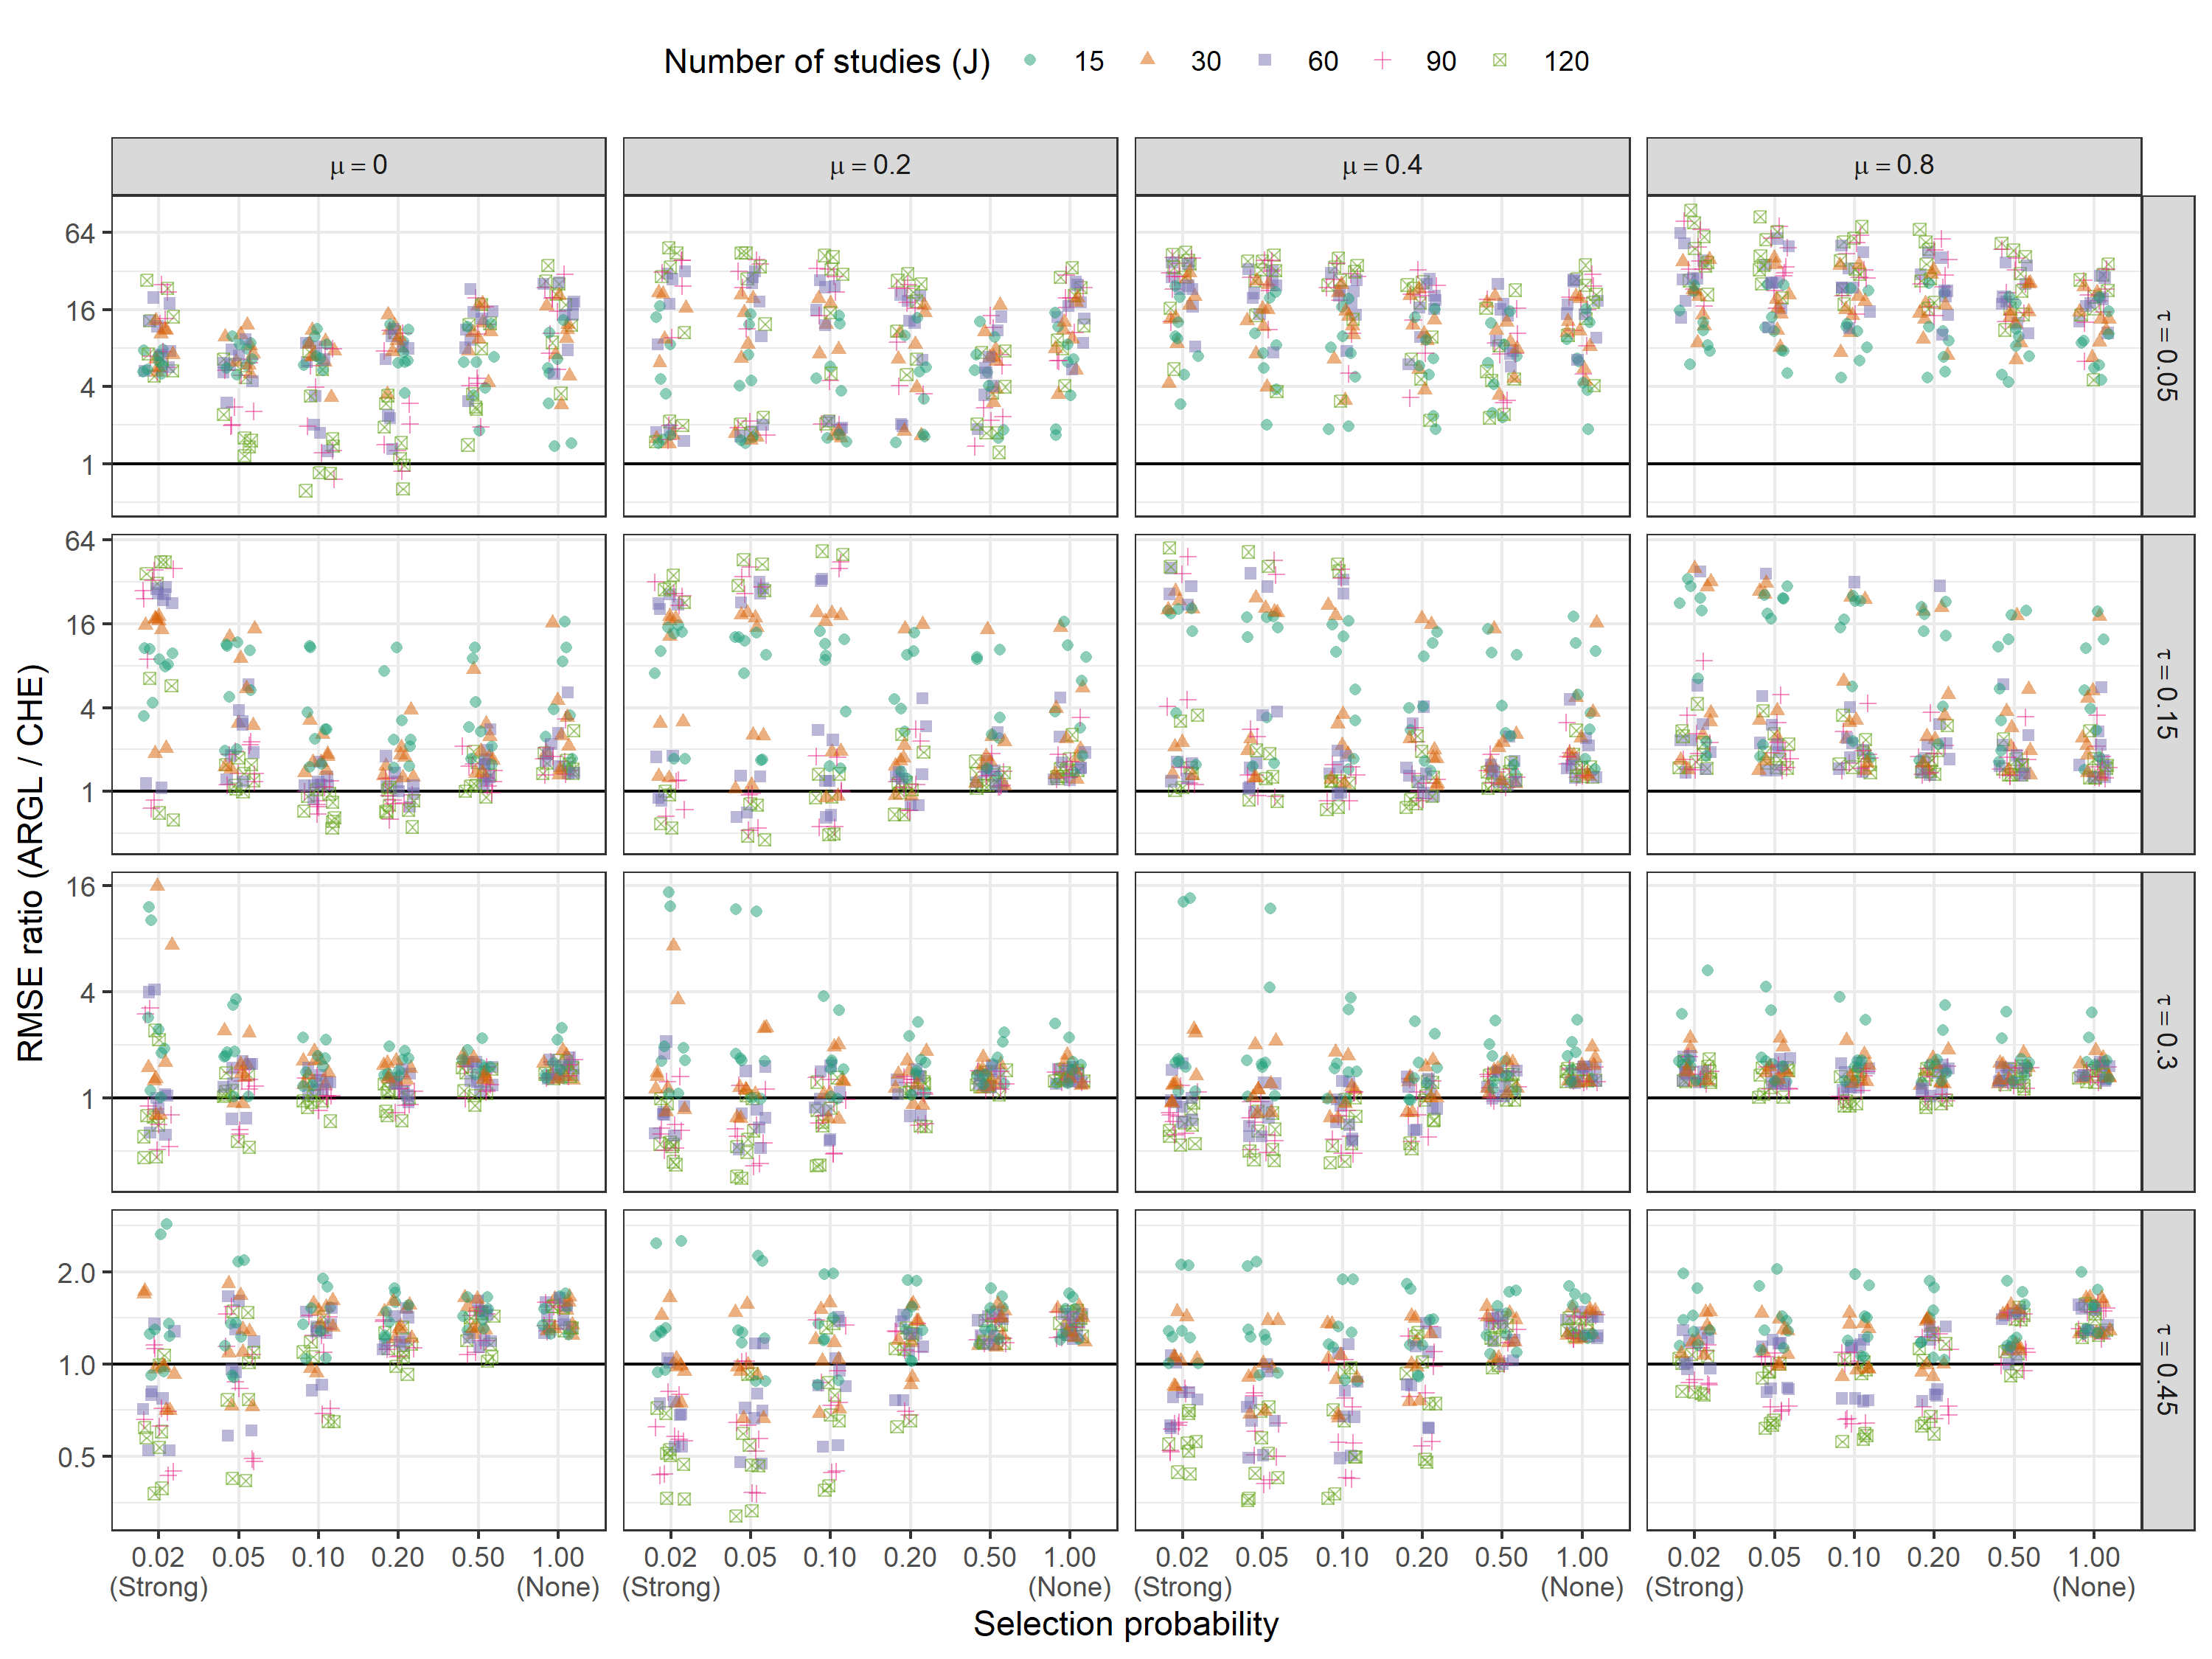
\includegraphics{selection_models_draft_files/figure-latex/heterogeneity-rmse-ARGL-CHE-1} \caption{Ratio of root mean-squared error for ARGL heterogeneity estimator to root mean-squared error of CHE heterogeneity estimator by selection probability, number of studies, average SMD, and between-study heterogeneity}\label{fig:heterogeneity-rmse-ARGL-CHE}
\end{sidewaysfigure}

\begin{sidewaysfigure}
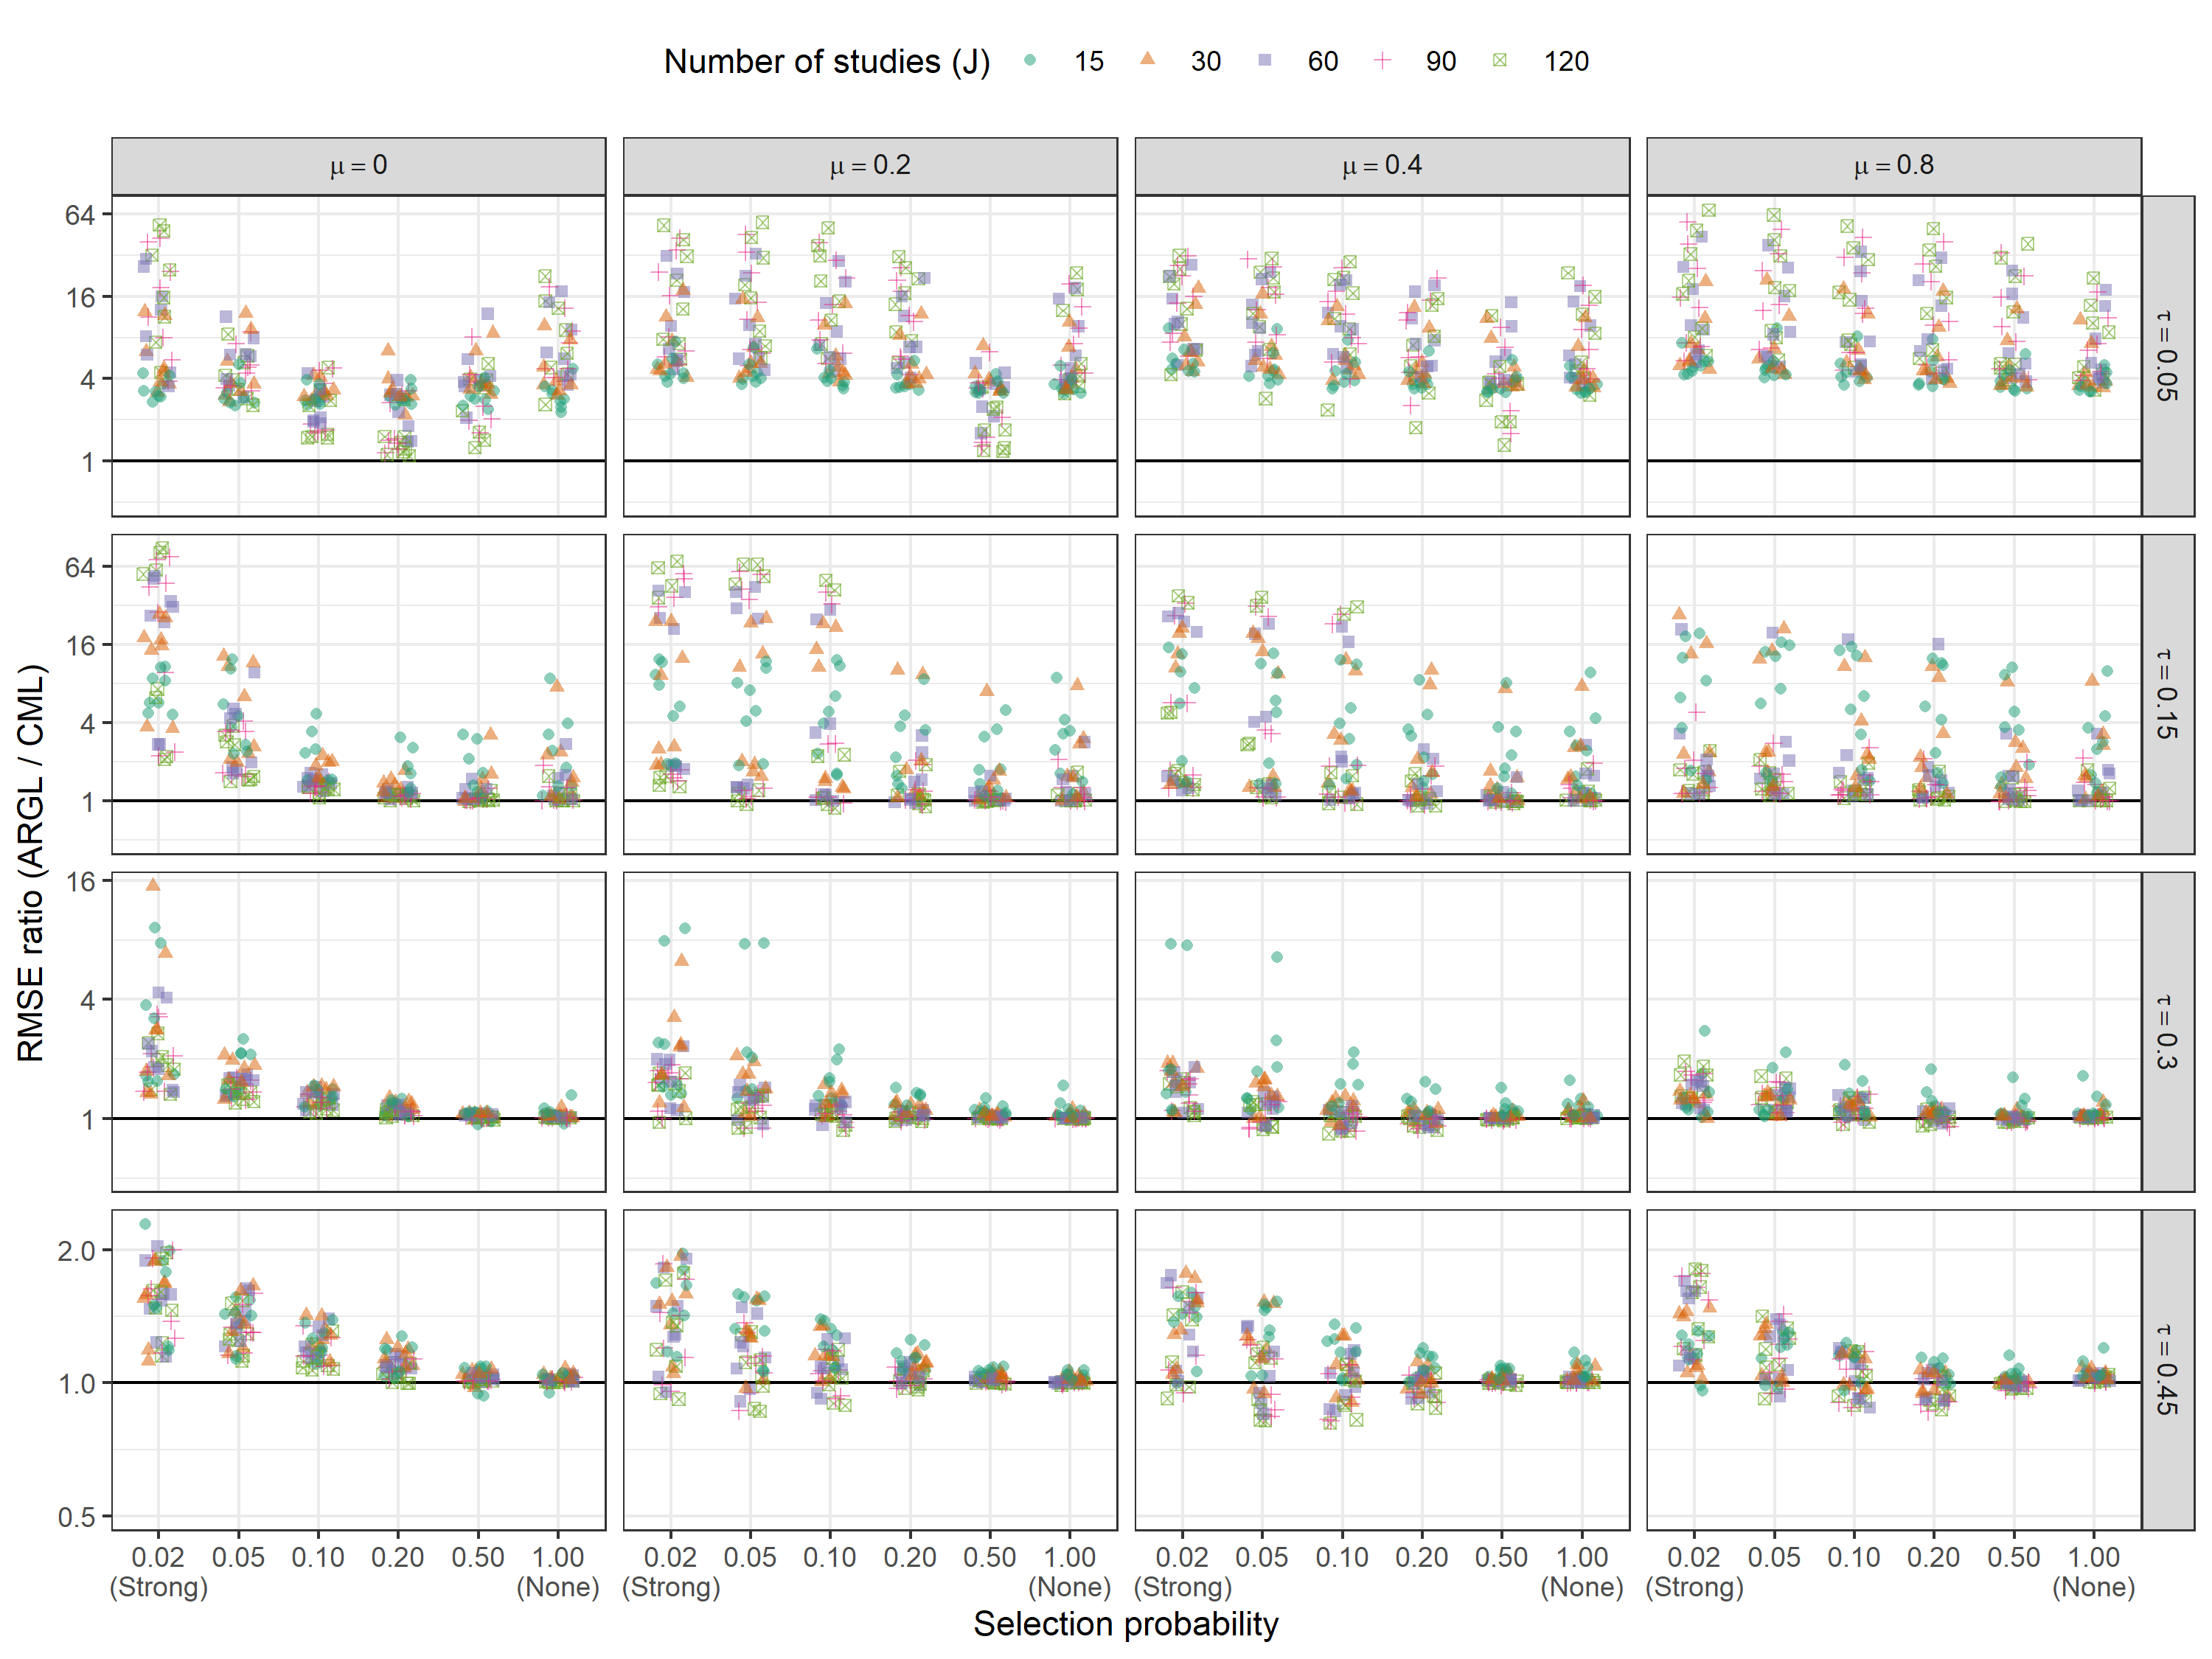
\includegraphics{selection_models_draft_files/figure-latex/heterogeneity-rmse-ARGL-CML-1} \caption{Ratio of root mean-squared error for ARGL heterogeneity estimator to root mean-squared error of CML heterogeneity estimator by selection probability, number of studies, average SMD, and between-study heterogeneity}\label{fig:heterogeneity-rmse-ARGL-CML}
\end{sidewaysfigure}

\section{\texorpdfstring{Additional simulation results for estimators of selection parameter \((\zeta_1)\)}{Additional simulation results for estimators of selection parameter (\textbackslash zeta\_1)}}\label{zeta-simulation-results}

\begin{sidewaysfigure}
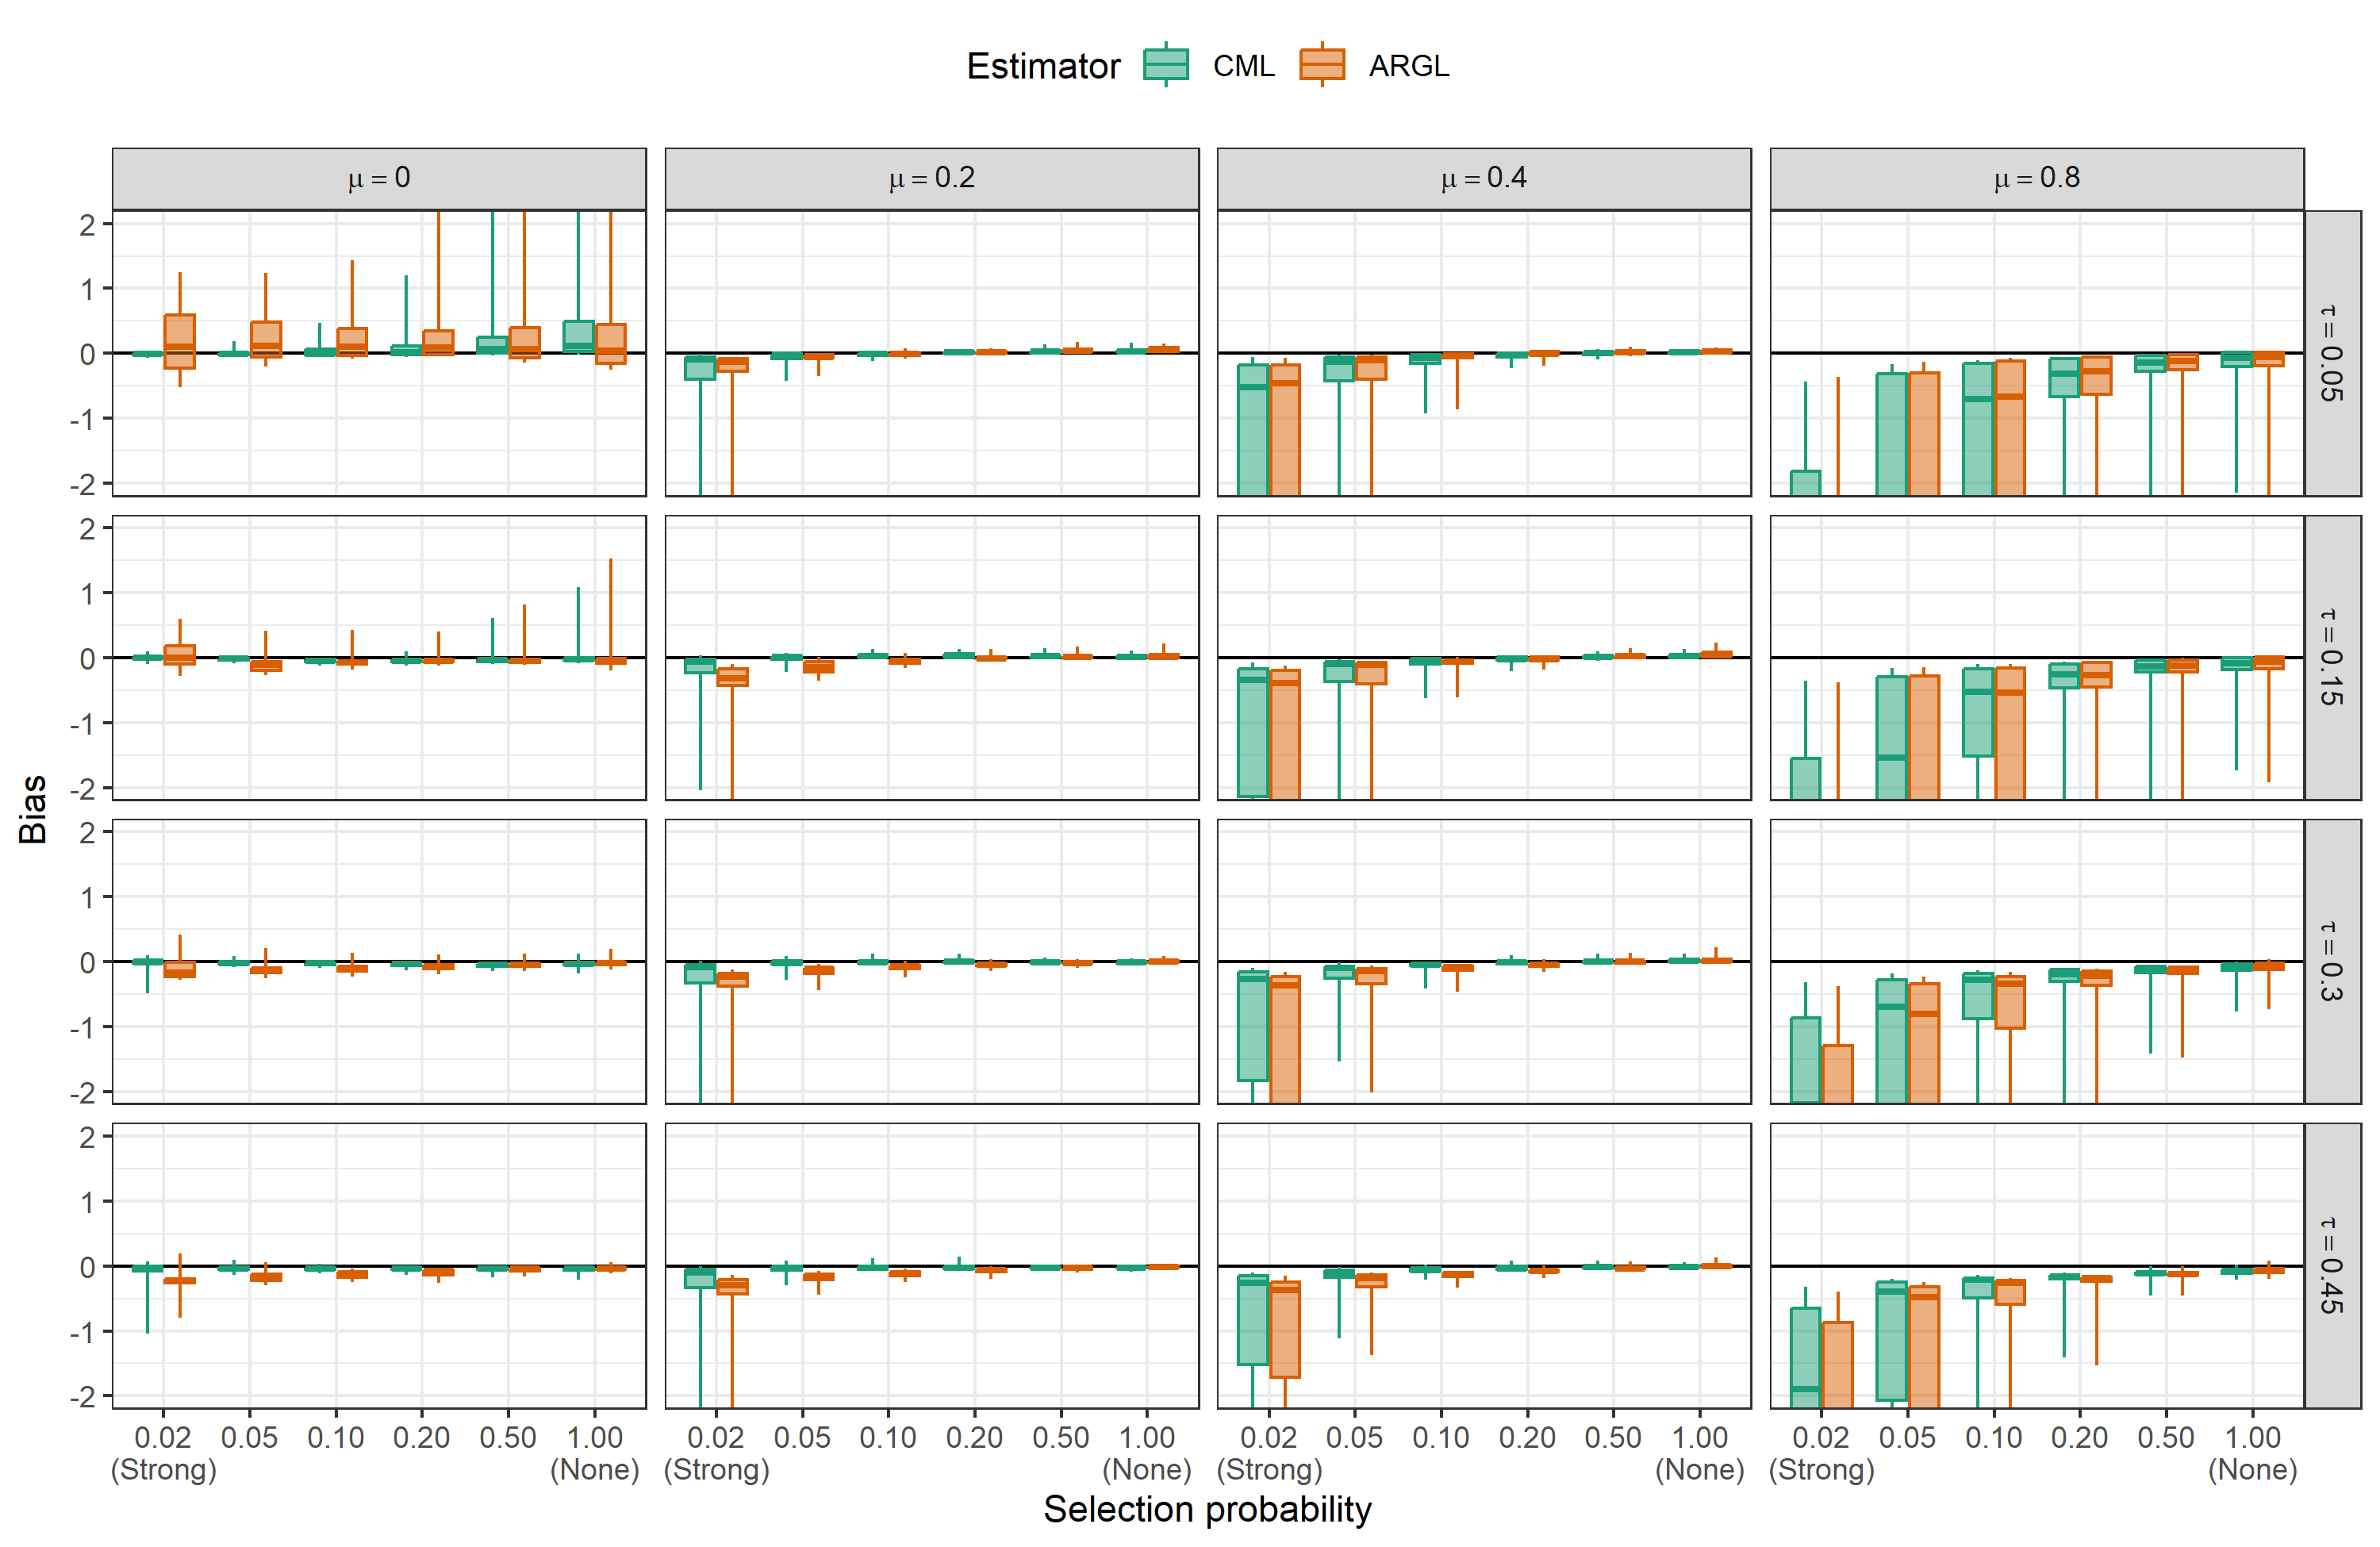
\includegraphics{selection_models_draft_files/figure-latex/selection-bias-1} \caption{Bias for estimators of log-selection parameter by selection probability, average SMD, and between-study heterogeneity}\label{fig:selection-bias}
\end{sidewaysfigure}

\begin{sidewaysfigure}
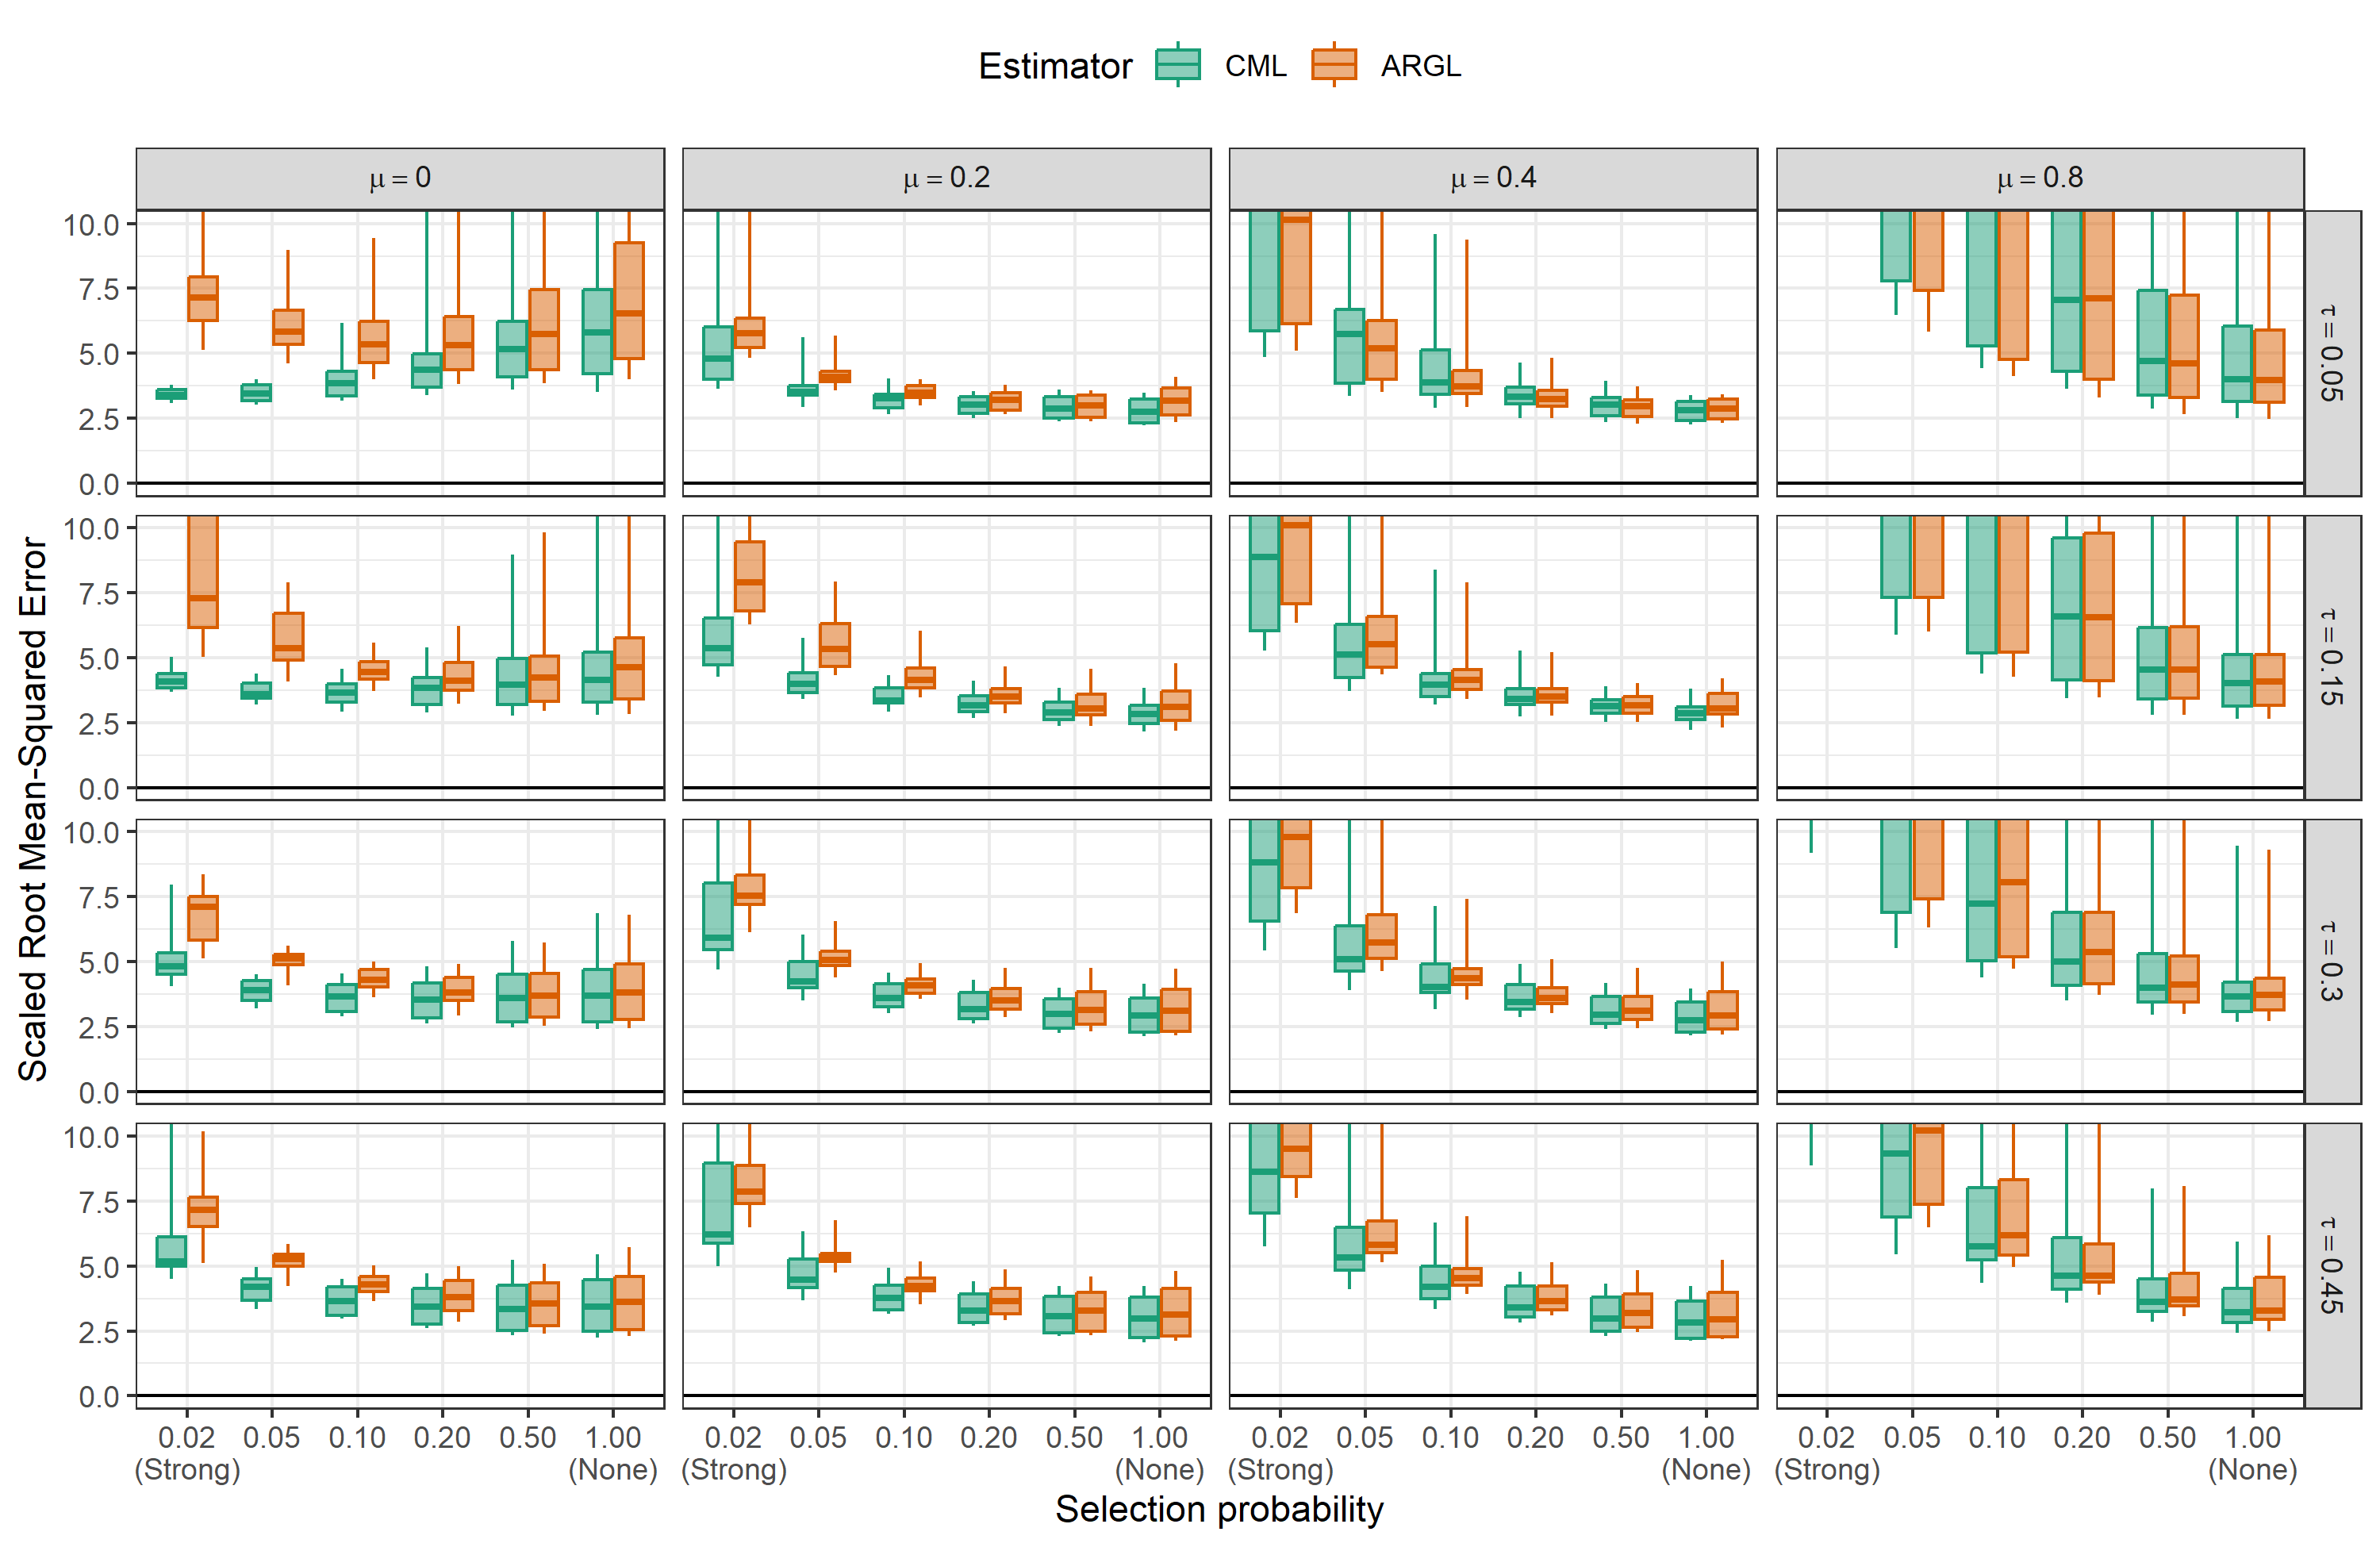
\includegraphics{selection_models_draft_files/figure-latex/selection-rmse-1} \caption{Scaled root mean-squared error for log-selection parameter estimators by selection probability, average SMD, and between-study heterogeneity}\label{fig:selection-rmse}
\end{sidewaysfigure}

\begin{sidewaysfigure}
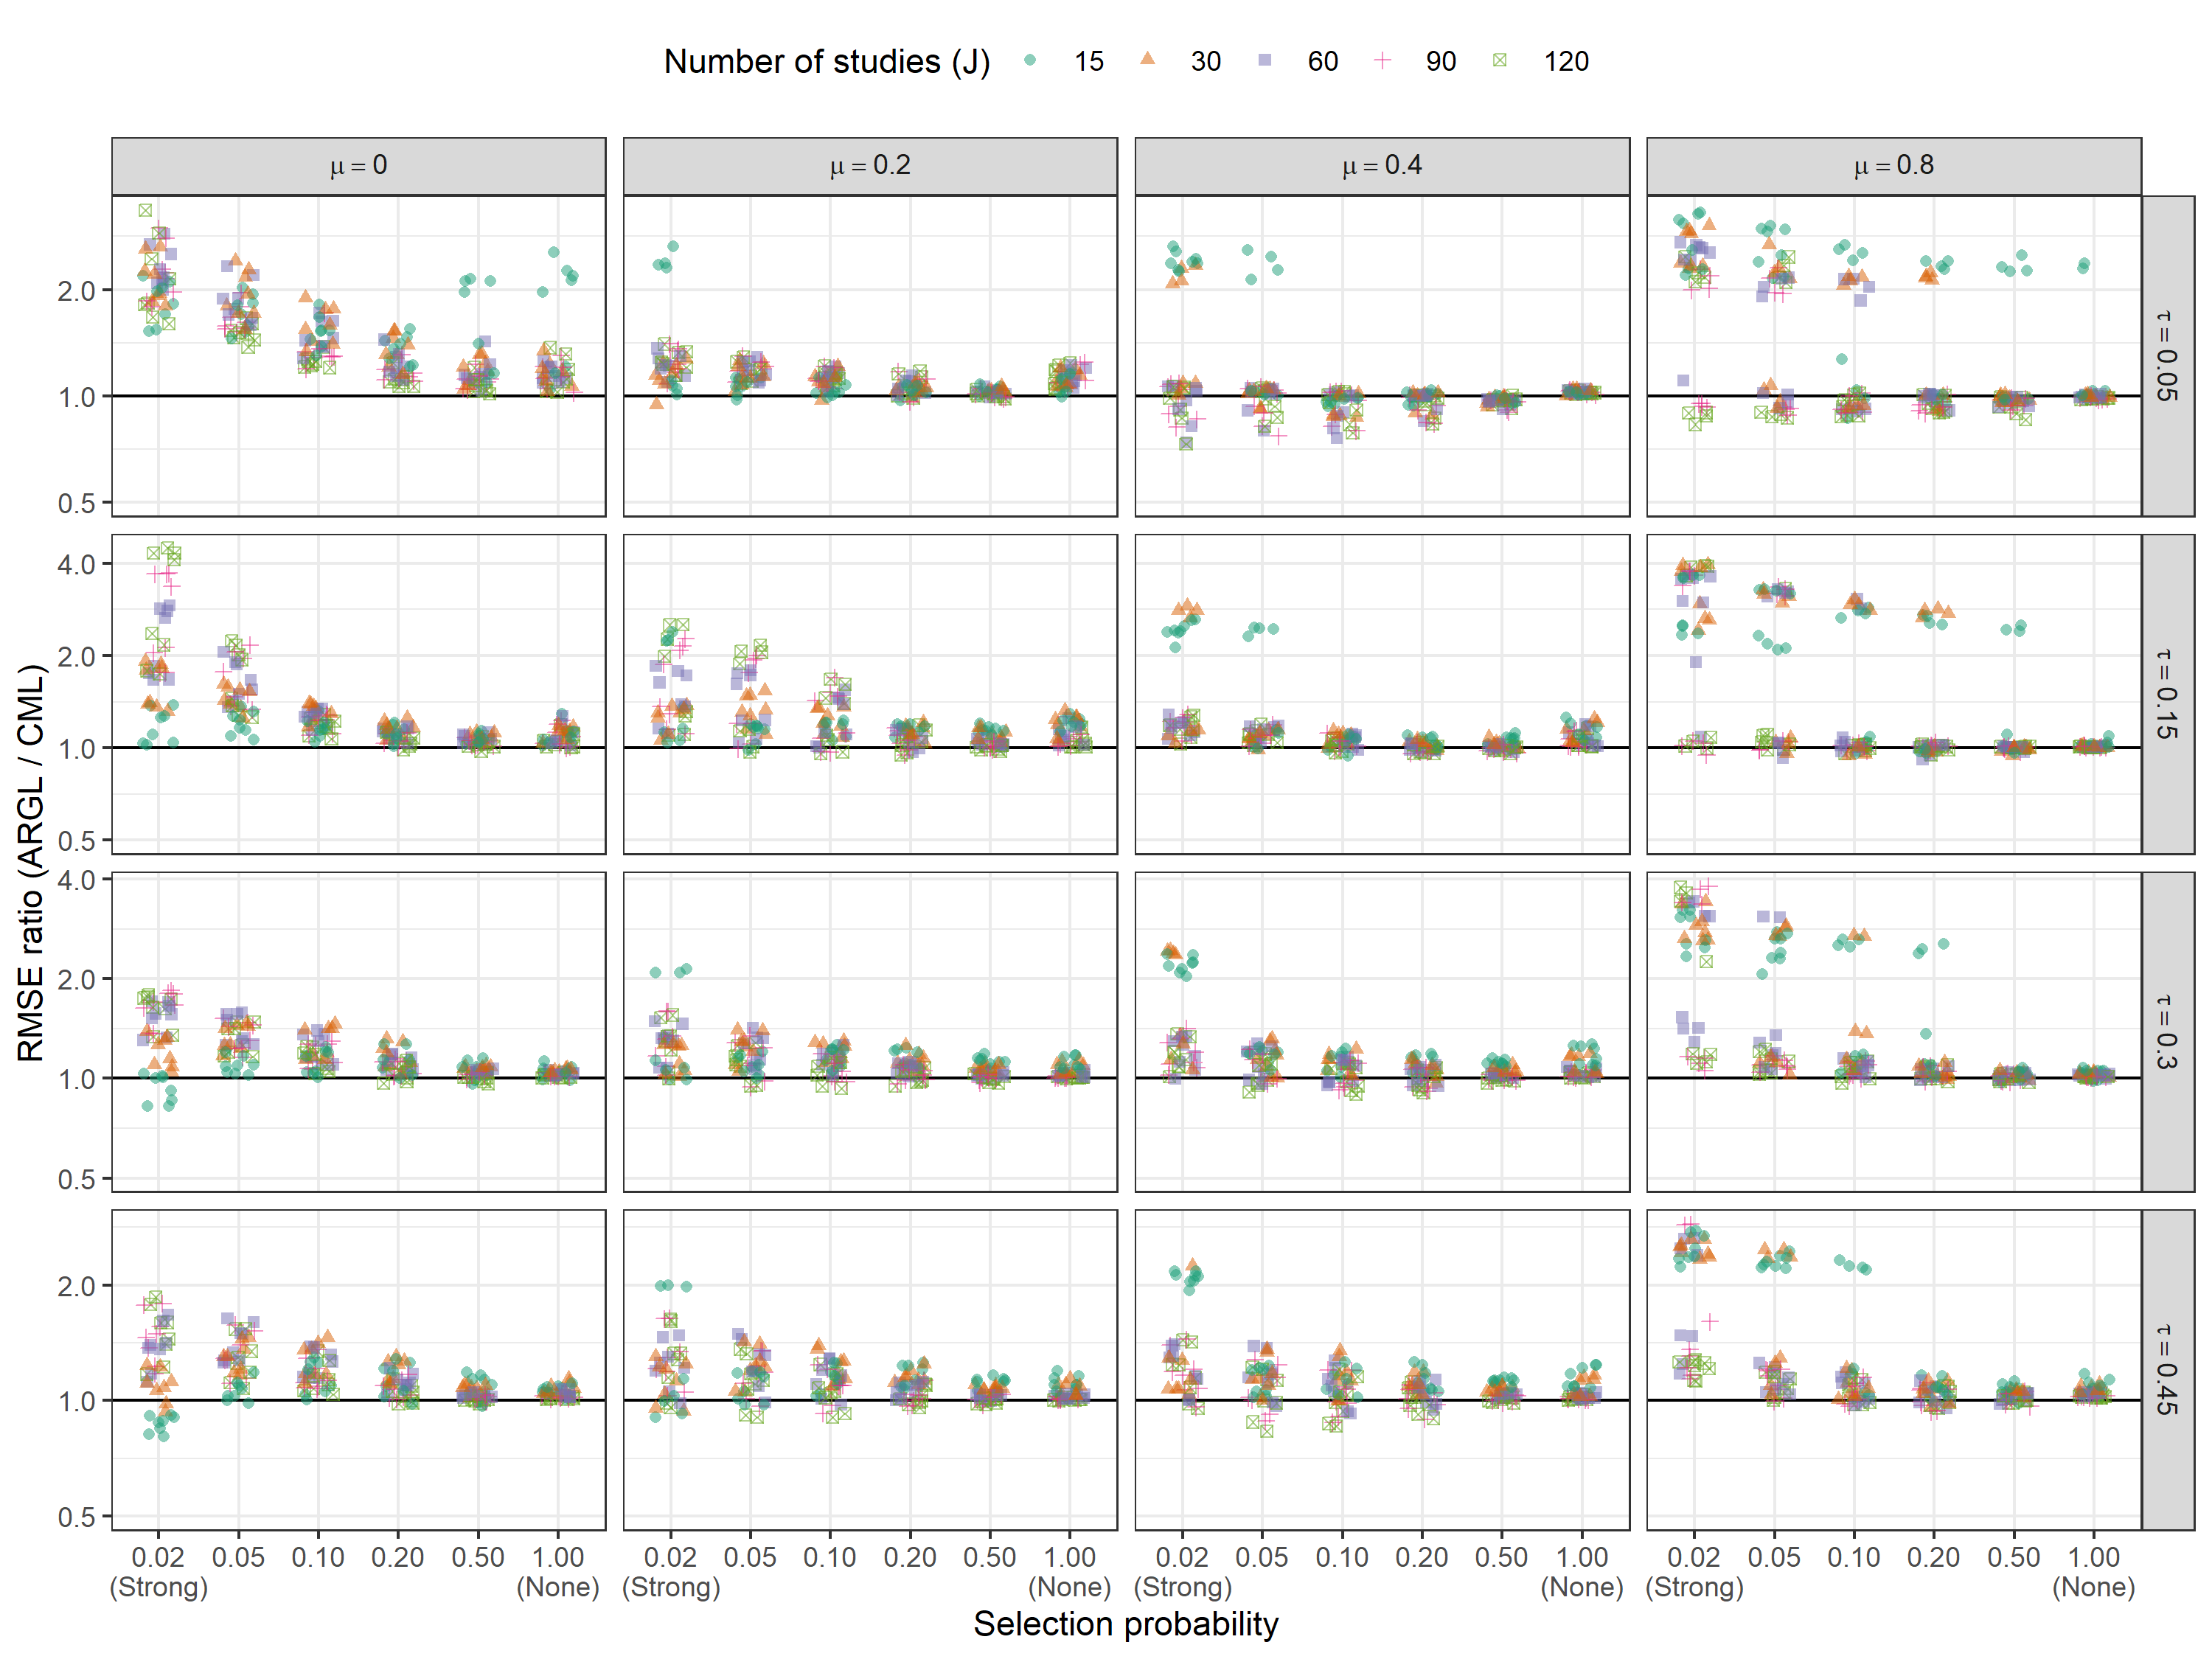
\includegraphics{selection_models_draft_files/figure-latex/selection-rmse-ARGL-CML-1} \caption{Ratio of root mean-squared error for ARGL log-selection parameter estimator to root mean-squared error of CML log-selection parameter estimator by selection probability, number of studies, average SMD, and between-study heterogeneity}\label{fig:selection-rmse-ARGL-CML}
\end{sidewaysfigure}

\begin{sidewaysfigure}
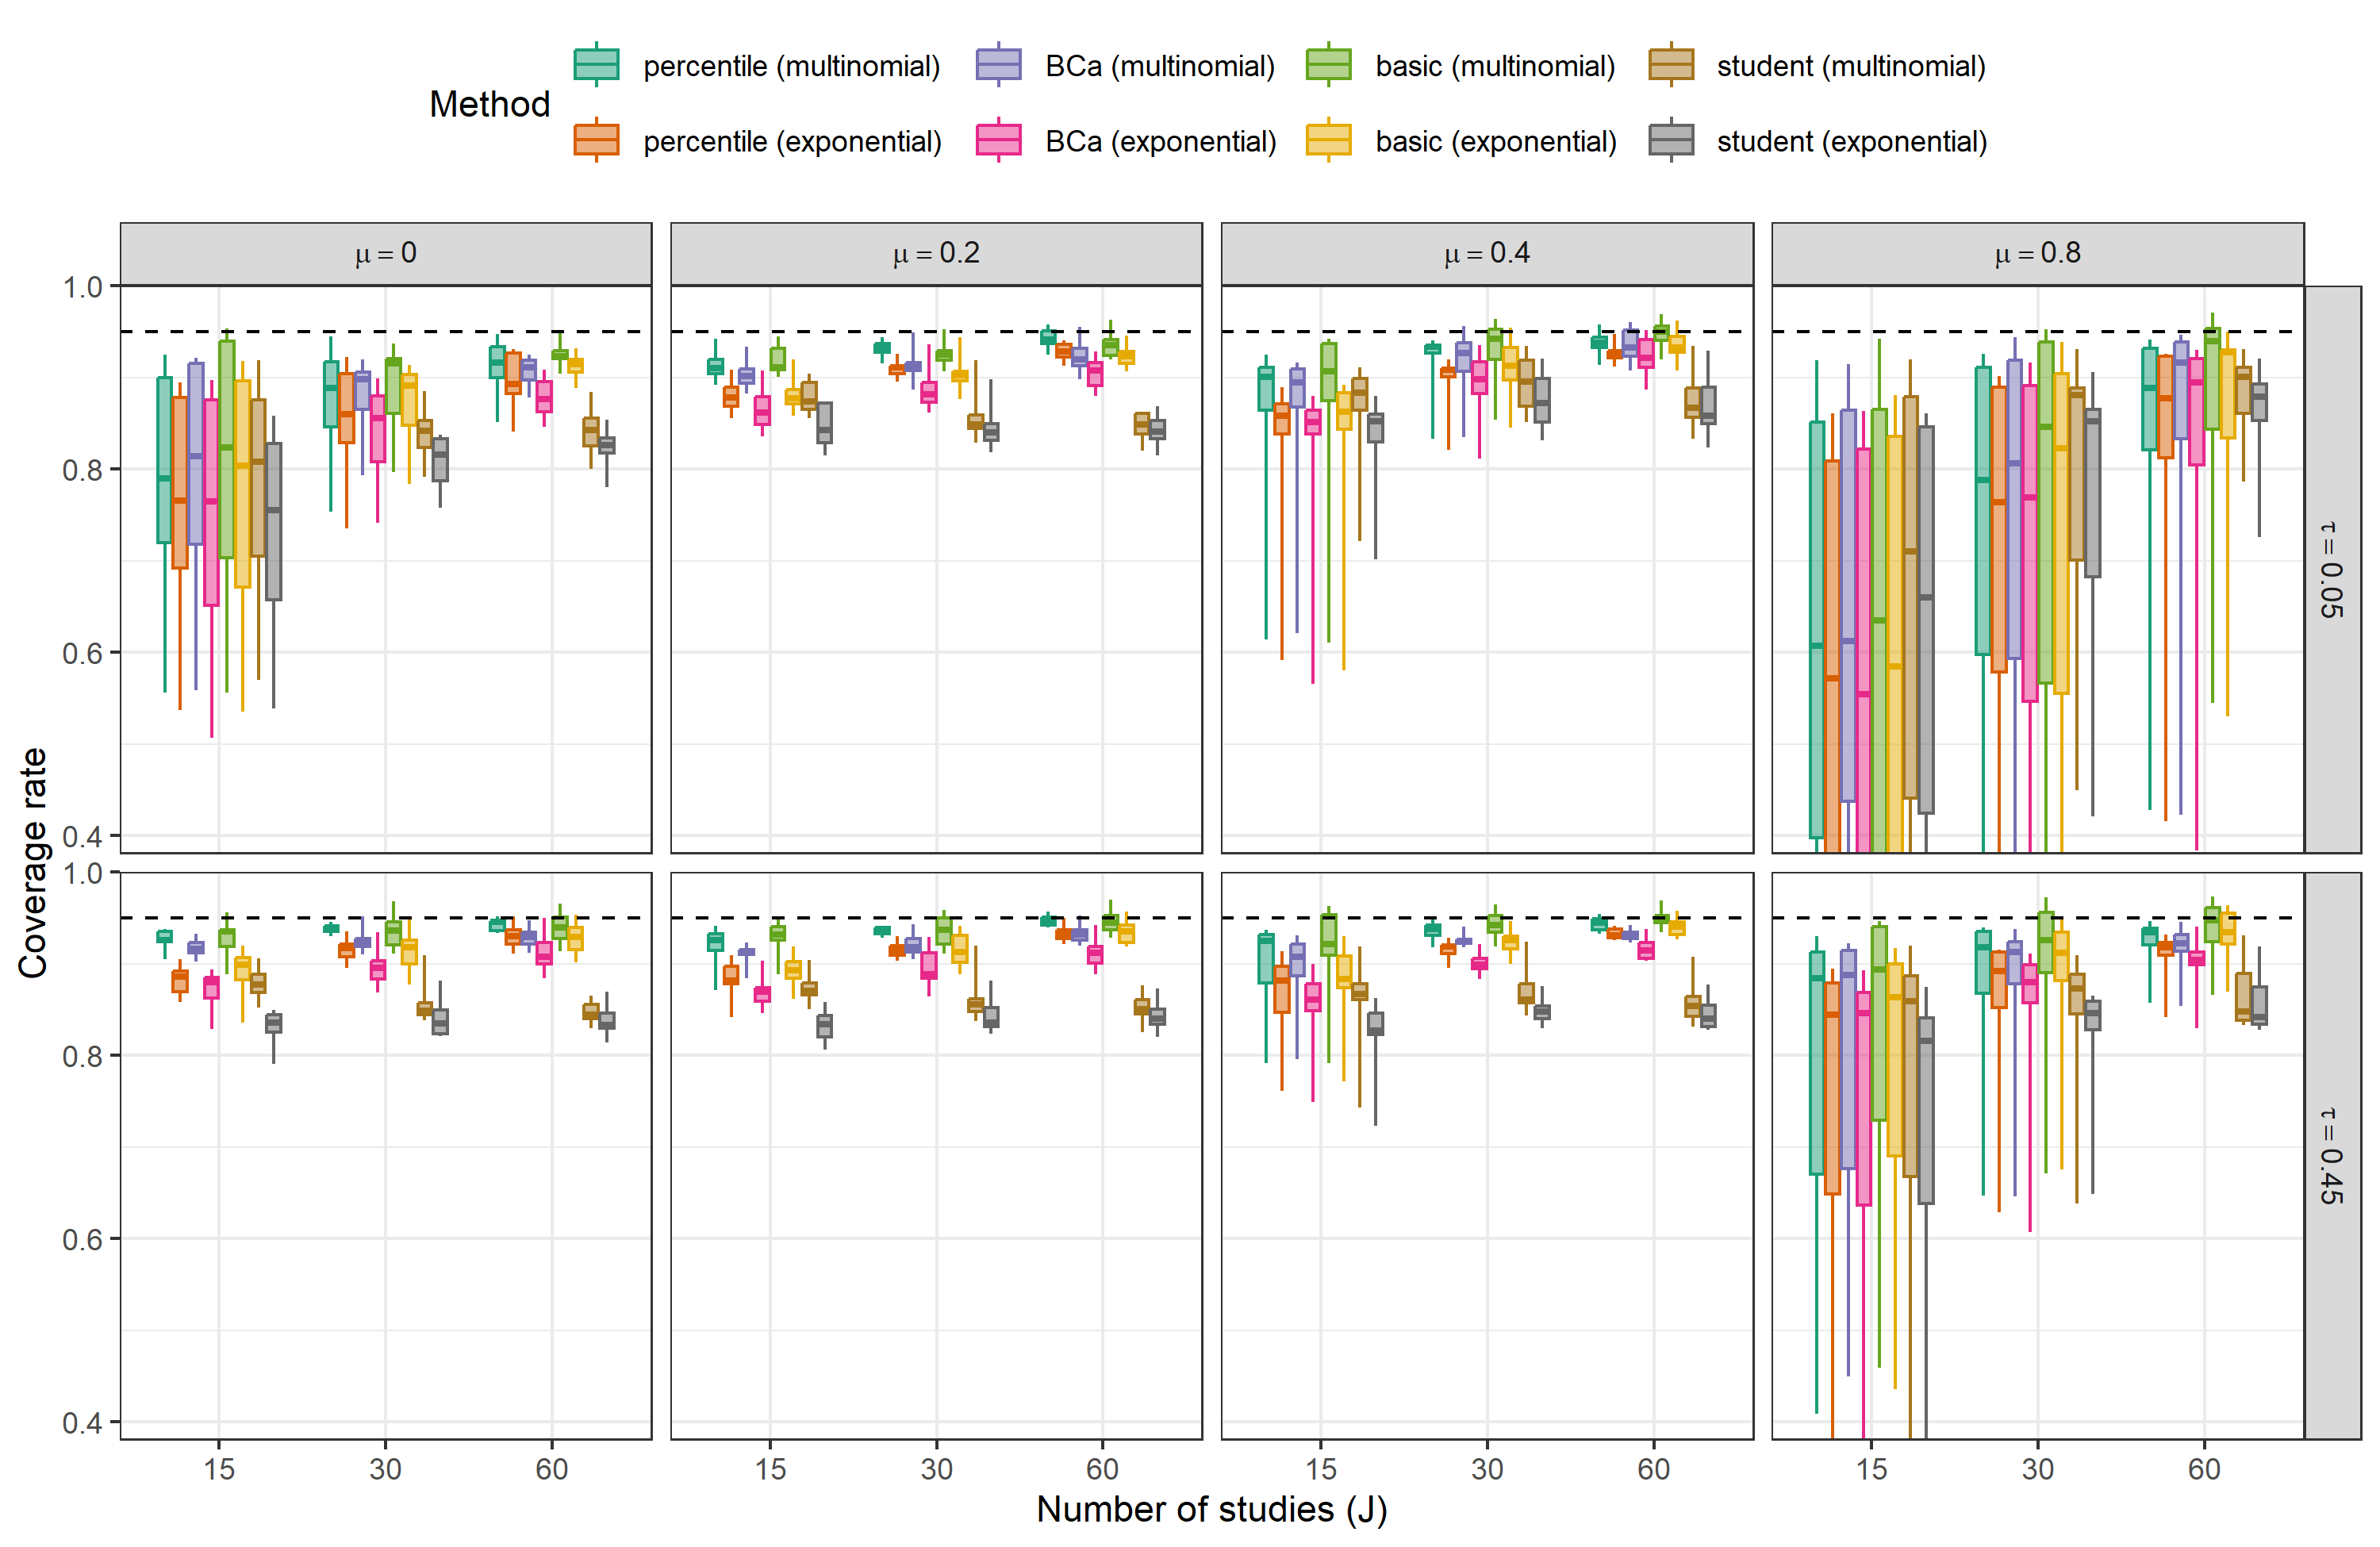
\includegraphics{selection_models_draft_files/figure-latex/CML-zeta-coverage-full-1} \caption{Coverage levels of bootstrap confidence intervals based on the CML estimator of log-selection parameter by number of studies, average SMD, and between-study heterogeneity. Dashed lines correspond to the nominal confidence level of 0.95.}\label{fig:CML-zeta-coverage-full}
\end{sidewaysfigure}

\begin{sidewaysfigure}
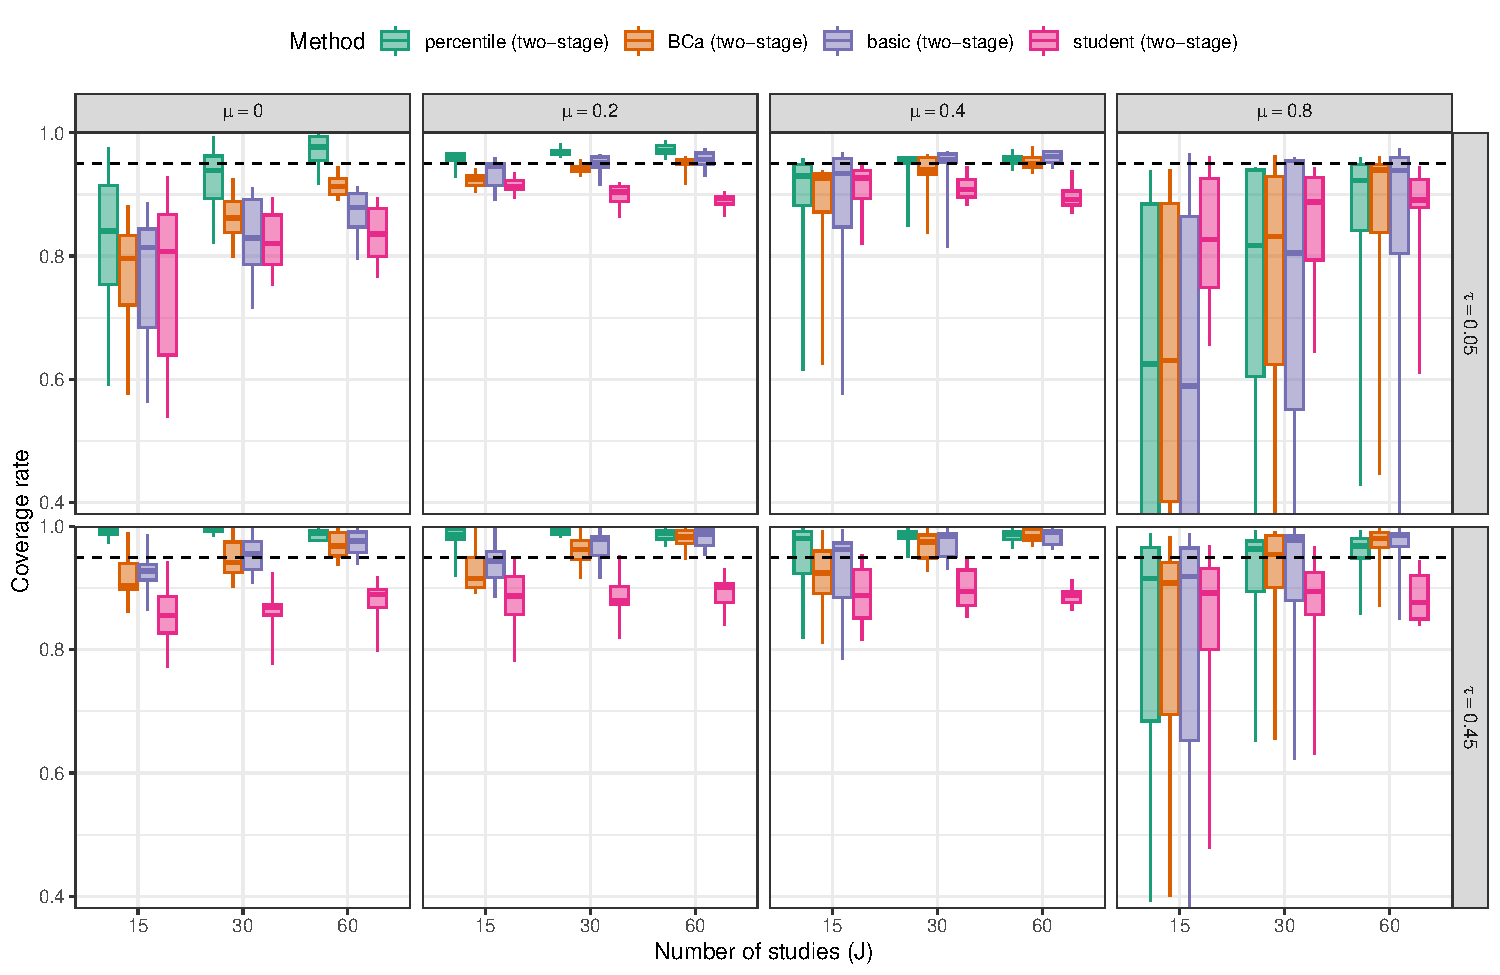
\includegraphics{selection_models_draft_files/figure-latex/ARGL-zeta-coverage-full-1} \caption{Coverage levels of bootstrap confidence intervals based on the ARGL estimator of log-selection parameter by number of studies, average SMD, and between-study heterogeneity. Dashed lines correspond to the nominal confidence level of 0.95.}\label{fig:ARGL-zeta-coverage-full}
\end{sidewaysfigure}


\end{document}
